% Soubory musí být v kódování, které je nastaveno v příkazu \usepackage[...]{inputenc}

\documentclass[%        Základní nastavení
%  draft,    				  % Testovací překlad
  12pt,       				% Velikost základního písma je 12 bodů
  a4paper,    				% Formát papíru je A4
  oneside,      			% Jednostranný tisk
	% twoside,      			% Dvoustranný tisk (kapitoly a další důležité části tedy začínají na lichých stranách)
	unicode,						% Záložky a metainformace ve výsledném  PDF budou v kódování unicode
]{report}				    	% Dokument třídy 'zpráva', vhodná pro sazbu závěrečných prací s kapitolami

\usepackage[utf8]		  %	Kódování zdrojových souborů je UTF-8
	{inputenc}					% Balíček pro nastavení kódování zdrojových souborů

\usepackage[				% Nastavení geometrie stránky
	bindingoffset=10mm,		% Hřbet pro vazbu
	hmargin={25mm,25mm},	% Vnitřní a vnější okraj  (jsou nehezky shodné; jakási úroveň estetiky je dosažena pomocí hřbetu)
	vmargin={25mm,34mm},	% Horní a dolní okraj
	footskip=17mm,			  % Velikost zápatí
	nohead,					      % Bez záhlaví
	marginparsep=2mm,		  % Vzdálenost marginálií
	marginparwidth=18mm,	% Šířka marginálií
]{geometry}

\usepackage{sectsty}
	%přetypuje nadpisy všech úrovní na bezpatkové, kromě \chapter, která je přenastavena zvlášť v thesis.sty
	\allsectionsfont{\sffamily}

\usepackage{graphicx} % Balíček 'graphicx' pro vkládání obrázků
											% Nutné pro vložení logotypů školy a fakulty

\usepackage[          % Balíček 'acronym' pro sazby zkratek a symbolů
	nohyperlinks				% Nebudou tvořeny hypertextové odkazy do seznamu zkratek
]{acronym}						
											% Nutné pro použití prostředí 'acronym' balíčku 'thesis'

\usepackage[
	breaklinks=true,		% Hypertextové odkazy mohou obsahovat zalomení řádku
	hypertexnames=false, % Názvy hypertext. odkazů budou tvořeny nezávisle na názvech TeXu
]{hyperref}						% Balíček 'hyperref' pro sazbu hypertextových odkazů
											% Nutné pro použití příkazu 'pdfsettings' balíčku 'thesis'

\usepackage{pdfpages} % Balíček umožňující vkládat stránky z PDF souborů
                      % Nutné při vkládání titulních listů a zadání přímo
                      % ve formátu PDF z informačního systému

\usepackage{enumitem} % Balíček pro nastavení mezerování v odrážkách
  \setlist{topsep=0pt,partopsep=0pt,noitemsep} % konkrétní nastavení

\usepackage{cmap} 		% Balíček cmap zajišťuje, že PDF vytvořené `pdflatexem' je
											% plně "prohledávatelné" a "kopírovatelné"

%\usepackage{upgreek}	% Balíček pro sazbu stojatých řeckých písmem
											%% např. stojaté pí: \uppi
											%% např. stojaté mí: \upmu (použitelné třeba v mikrometrech)
											%% pozor, grafická nekompatibilita s fonty typu Computer Modern!
                      
%\usepackage{amsmath} %balíček pro sabu náročnější matematiky                 

\usepackage{dirtree}	% sazba adresářové struktury
                      % vhodné pro prezentaci obsahu elektronické přílohy (např. CD)

\usepackage[formats]{listings}	% Balíček pro sazbu zdrojových textů
\lstset{              % nastavení
%	Definice jazyka použitého ve výpisech
%    language=[LaTeX]{TeX},	% LaTeX
%	language={Matlab},		% Matlab
	language={C},           % jazyk C
    basicstyle=\ttfamily,	% definice základního stylu písma
    tabsize=2,			% definice velikosti tabulátoru
    inputencoding=utf8,         % pro soubory uložené v kódování UTF-8
		columns=fixed,  %fixed nebo flexible,
		fontadjust=true %licovani sloupcu
    extendedchars=true,
    literate=%  definice symbolů s diakritikou
    {á}{{\'a}}1
    {č}{{\v{c}}}1
    {ď}{{\v{d}}}1
    {é}{{\'e}}1
    {ě}{{\v{e}}}1
    {í}{{\'i}}1
    {ň}{{\v{n}}}1
    {ó}{{\'o}}1
    {ř}{{\v{r}}}1
    {š}{{\v{s}}}1
    {ť}{{\v{t}}}1
    {ú}{{\'u}}1
    {ů}{{\r{u}}}1
    {ý}{{\'y}}1
    {ž}{{\v{z}}}1
    {Á}{{\'A}}1
    {Č}{{\v{C}}}1
    {Ď}{{\v{D}}}1
    {É}{{\'E}}1
    {Ě}{{\v{E}}}1
    {Í}{{\'I}}1
    {Ň}{{\v{N}}}1
    {Ó}{{\'O}}1
    {Ř}{{\v{R}}}1
    {Š}{{\v{S}}}1
    {Ť}{{\v{T}}}1
    {Ú}{{\'U}}1
    {Ů}{{\r{U}}}1
    {Ý}{{\'Y}}1
    {Ž}{{\v{Z}}}1
}

%%%%%%%%%%%%%%%%%%%%%%%%%%%%%%%%%%%%%%%%%%%%%%%%%%%%%%%%%%%%%%%%%
%%%%%%      !!! VLASTNÍ BALÍČKY A NASTAVENÍ !!!        %%%%%%%%%%
%%%%%%%%%%%%%%%%%%%%%%%%%%%%%%%%%%%%%%%%%%%%%%%%%%%%%%%%%%%%%%%%%
%====== Units =====
\usepackage{siunitx}
\sisetup{inter-unit-product =\ensuremath{\cdot}}
\sisetup{group-digits = integer}
\sisetup{output-decimal-marker = {,}}
\sisetup{exponent-product = \ensuremath{\cdot}}
\sisetup{separate-uncertainty}
\sisetup{tight-spacing = false}
\DeclareSIUnit\permille{\text{\textperthousand}}
%\sisetup{scientific-notation = true}
%\sisetup{round-mode=places,round-precision=4}
%\sisetup{evaluate-expression}

%====== Hyperlinky ====== 
\hypersetup{allbordercolors={1 1 1}}

%====== Obrazky ========
% \usepackage{graphicx} 
% \usepackage[dvipsnames]{xcolor} % E: option clash for package xcolor
% \usepackage{tikz}

% ^^ už tam někde prý jsou použité

\usepackage[siunitx]{circuitikz}
\usepackage{pgf}
\usetikzlibrary{matrix}
\usetikzlibrary{fit}
\usetikzlibrary{patterns}
\usepackage{tkz-euclide}
\usetikzlibrary{arrows.meta, bending, patterns.meta, ducks}
\usetikzlibrary{shapes, backgrounds, decorations.pathmorphing, calc}
\usetikzlibrary{positioning}

\usepackage{derivative} % nebude potřeba

\usepackage{pgfplots}
\pgfplotsset{width=0.8\linewidth, compat=1.17}
\def\plotcscale{0.8}
\usepackage{pgfplotstable}
\newcommand*\circled[1]{\tikz[baseline=(char.base)]{
            \node[shape=circle,draw,inner sep=1pt] (char) {#1};}}

\usepackage[style=iso-numeric,backend=biber]{biblatex}
\addbibresource{text/literatura.bib}
%making everything to match Juice citations
\DeclareFieldFormat{labelnumberwidth}{\mkbibbrackets{#1}}
% \usepackage{natbib}
% \usepackage{url}
% \DeclareUrlCommand\url{\def\UrlLeft{<}\def\UrlRight{>} \urlstyle{tt}}


% TEMP
\usepackage{multirow}
\usepackage{array}
\usepackage{tabularx}
\usepackage{calc}





%%%%%%%%%%%%%%%%%%%%%%%%%%%%%%%%%%%%%%%%%%%%%%%%%%%%%%%%%%%%%%%%%
%%%%%%      Definice informací o dokumentu             %%%%%%%%%%
%%%%%%%%%%%%%%%%%%%%%%%%%%%%%%%%%%%%%%%%%%%%%%%%%%%%%%%%%%%%%%%%%

% V tomto souboru se nastavují téměř veškeré informace, proměnné mezi studenty:
% jméno, název práce, pohlaví atd.
% Tento soubor je SDÍLENÝ mezi textem práce a prezentací k obhajobě -- netřeba něco nastavovat na dvou místech.

\usepackage[
%%% Z následujících voleb jazyka lze použít pouze jednu
  czech-english,		% originální jazyk je čeština, překlad je anglicky (výchozí)
  %english-czech,	% originální jazyk je angličtina, překlad je česky
  %slovak-english,	% originální jazyk je slovenština, překlad je anglicky
  %english-slovak,	% originální jazyk je angličtina, překlad je slovensky
%
%%% Z následujících voleb typu práce lze použít pouze jednu
  semestral,		  % semestrální práce (výchozí)
  %bachelor,			%	bakalářská práce
  %master,			  % diplomová práce
  %treatise,			% pojednání o disertační práci
  %doctoral,			% disertační práce
%
%%% Z následujících voleb zarovnání objektů lze použít pouze jednu
%  left,				  % rovnice a popisky plovoucích objektů budou zarovnány vlevo
	center,			    % rovnice a popisky plovoucích objektů budou zarovnány na střed (vychozi)
%
]{thesis}   % Balíček pro sazbu studentských prací


%%% Jméno a příjmení autora ve tvaru
%  [tituly před jménem]{Křestní}{Příjmení}[tituly za jménem]
% Pokud osoba nemá titul před/za jménem, smažte celý řetězec '[...]'
\author[]{Jakub}{Charvot}

%%% Identifikační číslo autora (VUT ID)
\butid{240844}

%%% Pohlaví autora/autorky
% (nepoužije se ve variantě english-czech ani english-slovak)
% Číselná hodnota: 1...žena, 0...muž
\gender{0}

%%% Jméno a příjmení vedoucího/školitele včetně titulů
%  [tituly před jménem]{Křestní}{Příjmení}[tituly za jménem]
% Pokud osoba nemá titul před/za jménem, smažte celý řetězec '[...]'
\advisor[Ing.]{Pavel}{Tomíček}[]

%%% Jméno a příjmení oponenta včetně titulů
%  [tituly před jménem]{Křestní}{Příjmení}[tituly za jménem]
% Pokud osoba nemá titul před/za jménem, smažte celý řetězec '[...]'
% Nastavení oponenta se uplatní pouze v prezentaci k obhajobě;
% v případě, že nechcete, aby se na titulním snímku prezentace zobrazoval oponent, pouze příkaz zakomentujte;
% u obhajoby semestrální práce se oponent nezobrazuje (jelikož neexistuje)
% U dizertační práce jsou typicky dva až tři oponenti. Pokud je chcete mít na titulním slajdu, prosím ručně odkomentujte a upravte jejich jména v definici "VUT title page" v souboru thesis.sty.
\opponent[doc.]{Oponent}{Krutý}[Ph.D.]

%%% Název práce
%  Parametr ve složených závorkách {} je název v originálním jazyce,
%  parametr v hranatých závorkách [] je překlad (podle toho jaký je originální jazyk).
%  V případě, že název Vaší práce je dlouhý a nevleze se celý do zápatí prezentace, použijte příkaz
%  \def\insertshorttitle{Zkác.\ náz.\ práce}
%  kde jako parametr vyplníte zkrácený název. Pokud nechcete zkracovat název, budete muset předefinovat,
%  jak se vytváří patička slidu. Viz odkaz: https://bit.ly/3EJTp5A
\title[Autonomous aquarium]{Autonomní akvárium}

%%% Označení oboru studia
%  Parametr ve složených závorkách {} je název oboru v originálním jazyce,
%  parametr v hranatých závorkách [] je překlad
\specialization[Microelectronics and Technology]{Mikroelektronika a technologie}

%%% Označení ústavu
%  Parametr ve složených závorkách {} je název ústavu v originálním jazyce,
%  parametr v hranatých závorkách [] je překlad
%\department[Department of Control and Instrumentation]{Ústav automatizace a měřicí techniky}
%\department[Department of Biomedical Engineering]{Ústav biomedicínského inženýrství}
%\department[Department of Electrical Power Engineering]{Ústav elektroenergetiky}
%\department[Department of Electrical and Electronic Technology]{Ústav elektrotechnologie}
%\department[Department of Physics]{Ústav fyziky}
%\department[Department of Foreign Languages]{Ústav jazyků}
%\department[Department of Mathematics]{Ústav matematiky}
\department[Department of Microelectronics]{Ústav mikroelektroniky}
%\department[Department of Radio Electronics]{Ústav radioelektroniky}
%\department[Department of Theoretical and Experimental Electrical Engineering]{Ústav teoretické a experimentální elektrotechniky}
% \department[Department of Telecommunications]{Ústav telekomunikací}
%\department[Department of Power Electrical and Electronic Engineering]{Ústav výkonové elektrotechniky a elektroniky}

%%% Označení fakulty
%  Parametr ve složených závorkách {} je název fakulty v originálním jazyce,
%  parametr v hranatých závorkách [] je překlad
%\faculty[Faculty of Architecture]{Fakulta architektury}
\faculty[Faculty of Electrical Engineering and~Communication]{Fakulta elektrotechniky a~komunikačních technologií}
%\faculty[Faculty of Chemistry]{Fakulta chemická}
%\faculty[Faculty of Information Technology]{Fakulta informačních technologií}
%\faculty[Faculty of Business and Management]{Fakulta podnikatelská}
%\faculty[Faculty of Civil Engineering]{Fakulta stavební}
%\faculty[Faculty of Mechanical Engineering]{Fakulta strojního inženýrství}
%\faculty[Faculty of Fine Arts]{Fakulta výtvarných umění}
%
%Nastavení logotypu (v hranatych zavorkach zkracene logo, ve slozenych plne):
\facultylogo[logo/FEKT_zkratka_barevne_PANTONE_CZ]{logo/UTKO_color_PANTONE_CZ}

%%% Rok odevzdání práce
\graduateyear{2024}
%%% Akademický rok odevzdání práce
\academicyear{2023/24}

%%% Datum obhajoby (uplatní se pouze v prezentaci k obhajobě)
\date{11.\,11.\,1980} 

%%% Místo obhajoby
% Na titulních stránkách bude automaticky vysázeno VELKÝMI písmeny (pokud tyto stránky sází šablona)
\city{Brno}

%%% Abstrakt
\abstract[%
This thesis delves into the topic of~aquarium automation, aiming to~design custom device for this purpose. A~market survey is~presented with depiction of~existing commercial solutions in~the~field of~automation, also the~essential technology requirements for~efficient aquarium operation are summarized. Regarding the~design of~the~custom device, the~thesis explain the~chosen architecture and takes a~deeper look at~some of~its~parts. The main outcome of~this thesis is the~creation of~an~electrical schematic for the~control unit. The~present work will be followed by a bachelor's thesis, within which the~device will be completed.
]{%
Tato práce se zaměřuje na problematiku automatizace akvárií a jejím cílem je navrhnout vlastní zařízení sloužící tomuto účelu. V práci je proveden trůzkum trhu a popsána již existující komerční řešení věnující se právě automatizaci, také je zde obsaženo shrnutí minimální techniky potřebné pro provoz akvária. Z hlediska návrhu vlastního zařízení je obsažen popis a odůvodnění zvolené architektury, dále se text detailněji věnuje některým dílčím blokům. Výstupem práce je zejména navržené elektrické schéma řídící jednotky. Na tuto práci bude navazovat bakalářská práce, v rámci které bude zařízení dokončeno. 
}

%%% Klíčová slova
\keywrds[%
aquaristics, automation, ESP32, data buses, device design
]{%
akvaristika, automatizace, ESP32, sběrnice, návrh zařízení
}


%%% Poděkování
\acknowledgement{%
Rád bych poděkoval vedoucímu semestrální práce
panu Ing.~Pavlu Tomíčkovi\ za ochotu i trpělivost, kterou se mnou měl po celou dobu tvorby této práce, a za mnoho cenných a podnětných rad k její odborné i formální stránce. Dále děkuji svému kamarádovi Radku Jančičkovi za osvětu v oblasti akvaristiky. 

}%  % do tohoto souboru doplňte údaje o sobě, druhu práce, názvu...

%%%%%%%%%%%%%%%%%%%%%%%%%%%%%%%%%%%%%%%%%%%%%%%%%%%%%%%%%%%%%%%%%%%%%%%%

%%%%%%%%%%%%%%%%%%%%%%%%%%%%%%%%%%%%%%%%%%%%%%%%%%%%%%%%%%%%%%%%%%%%%%%%
%%%%%%     Nastavení polí ve Vlastnostech dokumentu PDF      %%%%%%%%%%%
%%%%%%%%%%%%%%%%%%%%%%%%%%%%%%%%%%%%%%%%%%%%%%%%%%%%%%%%%%%%%%%%%%%%%%%%
%% Při načteném balíčku 'hyperref' lze použít příkaz '\pdfsettings':
\pdfsettings
%  Nastavení polí je možné provést také ručně příkazem:
%\hypersetup{
%  pdftitle={Název studentské práce},    	% Pole 'Document Title'
%  pdfauthor={Autor studenstké práce},   	% Pole 'Author'
%  pdfsubject={Typ práce}, 						  	% Pole 'Subject'
%  pdfkeywords={Klíčová slova}           	% Pole 'Keywords'
%}
%%%%%%%%%%%%%%%%%%%%%%%%%%%%%%%%%%%%%%%%%%%%%%%%%%%%%%%%%%%%%%%%%%%%%%%

\pdfmapfile{=vafle.map}

%%%%%%%%%%%%%%%%%%%%%%%%%%%%%%%%%%%%%%%%%%%%%%%%%%%%%%%%%%%%%%%%%%%%%%%
%%%%%%%%%%%       Začátek dokumentu               %%%%%%%%%%%%%%%%%%%%%
%%%%%%%%%%%%%%%%%%%%%%%%%%%%%%%%%%%%%%%%%%%%%%%%%%%%%%%%%%%%%%%%%%%%%%%
\begin{document}
\pagestyle{empty} %vypnutí číslování stránek

%%% Vložení desek -- od září 2021 na žádost fakulty nepoužíváno
% \includepdf[pages=1]%  buďto generovaných informačním systémem
%   {pdf/student-desky}% název souboru nesmí obsahovat mezery!
%%% NEBO vytvoření desek z balíčku
%%\makecover
%%%
%\oddpage % při dvojstranném tisku přidá prázdnou stránku
%% kazdopádně ale:
\setcounter{page}{1} %resetovaní čítače stránek -- desky do číslování nezahrnujeme

%% Vložení titulního listu
\includepdf[pages=1]%    buďto generovaného informačním systémem
  {pdf/student-titulka}% název souboru nesmí obsahovat mezery!
%% NEBO vytvoření titulní stránky z balíčku
%\maketitle
%%
\oddpage  % při dvojstranném tisku se přidá prázdná stránka
   
%% Vložení zadání
\includepdf[pages=1]%   buďto generovaného informačním systémem
  {pdf/student-zadani}% název souboru nesmí obsahovat mezery!
%% NEBO lze vytvořit prázdný list příkazem ze šablony
%\patternpage{}%
%	{\sffamily\Huge\centering ZDE VLOŽIT LIST ZADÁNÍ}%
%	{\sffamily\centering Z~důvodu správného číslování stránek}
%%
\oddpage% při dvojstranném tisku se přidá prázdná stránka

%% Vysázení stránky s abstraktem
\makeabstract

% Vysázení stránky s rozšířeným abstraktem
% (pokud píšete práci v češtině či slovenštině, vložení rozšířeného abstraktu zrušte;
%  pro semestrální projekt také není potřeba rozšířený abstrakt uvádět)
% % Vysázení stránky s rozšířeným abstraktem
% (týká se pouze bc. a dp. prací psaných v angličtině, viz Směrnice rektora 72/2017)
\cleardoublepage
\noindent
{\large\sffamily\bfseries\MakeUppercase{Rozšířený abstrakt}}
\\
Výtah ze směrnice rektora 72/2017:\\
\emph{Bakalářská a diplomová práce předložená v angličtině musí obsahovat rozšířený abstrakt v češtině
nebo slovenštině (čl. 15). To se netýká studentů, kteří studují studijní program akreditovaný v
angličtině.}
(čl. 3, par. 7)\\
\emph{Nebude-li vnitřní normou stanoveno jinak, doporučuje se rozšířený abstrakt o rozsahu přibližně 3
normostrany, který bude obsahovat úvod, popis řešení a shrnutí a~zhodnocení výsledků.}
(čl. 15, par. 5)

%%% Vysázení citace práce
\makecitation

%%% Vysázení prohlášení o samostatnosti
\makedeclaration

%%% Vysázení poděkování
\makeacknowledgement

%%% Vysázení obsahu
\tableofcontents

%%% Vysázení seznamu obrázků
% (vynechejte, pokud máte dva nebo méně obrázků)
\listoffigures

%%% Vysázení seznamu tabulek
% (vynechejte, pokud máte dvě nebo méně tabulek)
\listoftables

%%% Vysázení seznamu výpisů kódu
% (vynechejte, pokud máte dva nebo méně výpisů)
% \lstlistoflistings

\cleardoublepage\pagestyle{plain}   % zapnutí číslování stránek


%%%%%%%%%%%%%%%%%%%%%%%%%%%%%%%%%%%%%%%%%%%%%%%%%%%%%%%%%%%%%%%%%
%%%%%%%%%            SAMOTNÉ TEXTY PRÁCE             %%%%%%%%%%%%
%%%%%%%%%%%%%%%%%%%%%%%%%%%%%%%%%%%%%%%%%%%%%%%%%%%%%%%%%%%%%%%%%

\chapter*{Úvod}
\phantomsection
\addcontentsline{toc}{chapter}{Úvod}


V dnešní době, kdy jsou na vzestupu fenomény jako chytrá domácnost, \acs{iot} (\acl{iot}) nebo Průmysl 4.0, se na trhu objevuje stále více výrobků, které se snaží automatizovat a zjednodušit různé oblasti našeho života. Tento trend se dnes dotýká nejedné volnočasové aktivity a to včetně akvaristiky. Tu lze samozřejmě provozovat na různé úrovni, ale i majitelé malých domácích akvárií potřebují k provozu svého koníčku relativně velké množství elektroniky. 
Běžnou praxí je, že každé z použitých zařízení je ovládáno buďto zcela ručně nebo, pokud disponuje možností vzdáleného přístupu a automatizace, má svou samostanou aplikaci a uživatel tak provoz akvária musí ovládat z několika různých míst, což může být značně nepohodlné a nepřehledné.

Na trhu samozřejmě existují také velmi sofistikované a komplexní systémy, ty ovšem svou cenou vysoce přesahují rozpočet běžného "domácího" akvaristy. Tato práce se věnuje návrhu a tvorbě zařízení, které má za cíl nabídnout pohodlnou kontrolu a ovládání všech potřebných součástí domácího akvária, a to při zachování jednoduchosti a nízké pořizovací ceny.

% \input{text/images/CMOS_images.tex}

\chapter{Základní teorie akvaristiky}
    Tato kapitola je teoretickou částí práce, která předchází návrhu samotného zařízení. Na základě dostupných zdrojů jsou zde rozebrány technické požadavky na provoz akvária a proveden průzkum trhu v oblasti akvaristiky a její automatizace.  

\section{Historie}
    Pro lepší orientaci čtenáře ve trendech vývoje akvaristiky se práce nejprve zaměřuje na krátké shrnutí její historie. Kapitola slouží taképro pochopení motivace akvaristů k~rozvoji používané techniky.
\subsection{Počátky}
Akvaristika v~různých podobách provází lidstvo téměř od prvopočátku. Nejprve se jednalo spíše o~chov ryb užitkových, tedy rybářství, ovšem už ve starověké Mezopotámii docházelo také k~chovu ryb okrasných. Počátky akvaristiky byly prováděny spíše metodou pokusů a omylů, protože lidem nebyla známa velká část přírodních zákonitostí -- životní potřeby chovaných ryb, způsob jejich rozmnožování a v~neposlední řadě také procesy, odehrávající se v~přírodním ekosystému, zajišťující jeho rovnováhu. Základem udržení chovaných ryb naživu byla zejména častá výměna vody, ani tak ale dlouho nebylo možné udržet ryby při životě dlouhodobě. 

V~období středověku se poprvé objevuje také dovoz exotických okrasných rybek z~cizích zemí, pro naprostý nedostatek znalostí ale často brzy hynou, např. jen proto, že chovatele nenapadne je nakrmit~\cite{vitek_akvaristika}.

\subsection{Věda a technika}
Na konci 18. století dochází k~rozvoji vědy a několika objevům, které historii akvaristiky zásadně ovlivnily. Poprvé byl izolován kyslík, byl objasněn princip dýchání živočichů a následně také fotosyntéza. Akvaristika, v~tehdejší době umělý chov ryb za účelem pozorování a výzkumu, byla provozována zejména na vědecké půdě a byl zde zájem o~zdokonalení používaných technik a postupů. V~roce 1837 S. H. Ward prakticky prokázal, že osvětlené akvárium obsahující jak rybky, tak i rostliny, vydrží velmi dlouho bez nutnosti výměny vody~\cite{vitek_akvaristika}. Pricip výměny plynů byl významným milníkem ve snaze dosáhnout v~akváriu rovnováhy podobné přírodnímu prostředí. 

Při stále nových poznatcích o~životních potřebách ryb a o~akvarijní rovnováze bylo nutné přijít s~různými technickými řešeními. Akvária 19. a 20. století už byla vytápěná a uměle okysličovaná. Původní mechanická řešení a lihové kahany byly postupně nahrazovány elektrickými přístroji. V~pozdějších letech pak přibylo i umělé osvětlení a systémy filtrace vody. 
\section{Rozdělení akvárií}
TODO
\section{Technické vybavení akvária}
    V~této kapitole je uveden výčet základní akvaristické techniky nutné k~provozu domácího akvária, rozčleněné podle svého účelu. Ve druhé části se text věnuje přehledu různých dostupných komplexních systémů zaměřujících se na automatizaci provozu akvária. Cílem kapitoly je seznámit čtenáře blíže s~problematikou založení a provozu akvária a různými možnostmi technického zajištění jak domácích, tak i profesionálních akvárií.
    \subsection{Filtrace vody}
        Úkolem filtru je průběžně odstraňovat z~vody nečistoty, a to jak mechanické, tak zejména v~podobě škodlivých látek vznikajících v~akváriu. Filtrační materiál je volen tak, aby tvořil vhodné prostředí pro život filtračních bakterií, které se těmito škodlivými látkami živí \cite{yt-filtrace}. Rozlišujeme tři základní typy akvarijních filtrů -- vnější, vnitřní a závěsné. Na obr.~\ref{fig:filtry-srovnani} se nachází ukázka vybraných zástupců jednotlivých typů.
        
        \textbf{Vnějším filtrem} se rozumí zařízení umístěné obvykle ve skříňce pod akváriem, mívá připojeny dvě hadice -- na vstup a výstup vody. Toto řešení je považováno za nejlepší, protože filtr není omezen rozměry a může tak dosahovat daleko vyššího výkonu a účinnější filtrace díky většímu množství filtračních materiálů. 

        \textbf{Vnitřní filtr} (někdy také ponorný) je levným, ale nepříliš účinným řešením pro malá akvária. Nachází se z~velké části v~akváriu a za pomocí motorku tlačí vodu přes obvykle molitanovou náplň.

        \textbf{Závěsný filtr}  je kompromisním řešením.  Cenou i účinností filtrace se pohybuje mezi oběma zmíněnými typy. Nezabírá prostor uvnitř akvária a může tak využít větší objem filtrační hmoty než filtr vnitřní. Instalace je provedena zavěšením na stěnu akvária, je tedy velmi jednoduchá. 

        \begin{figure}[h!]
            \centering
            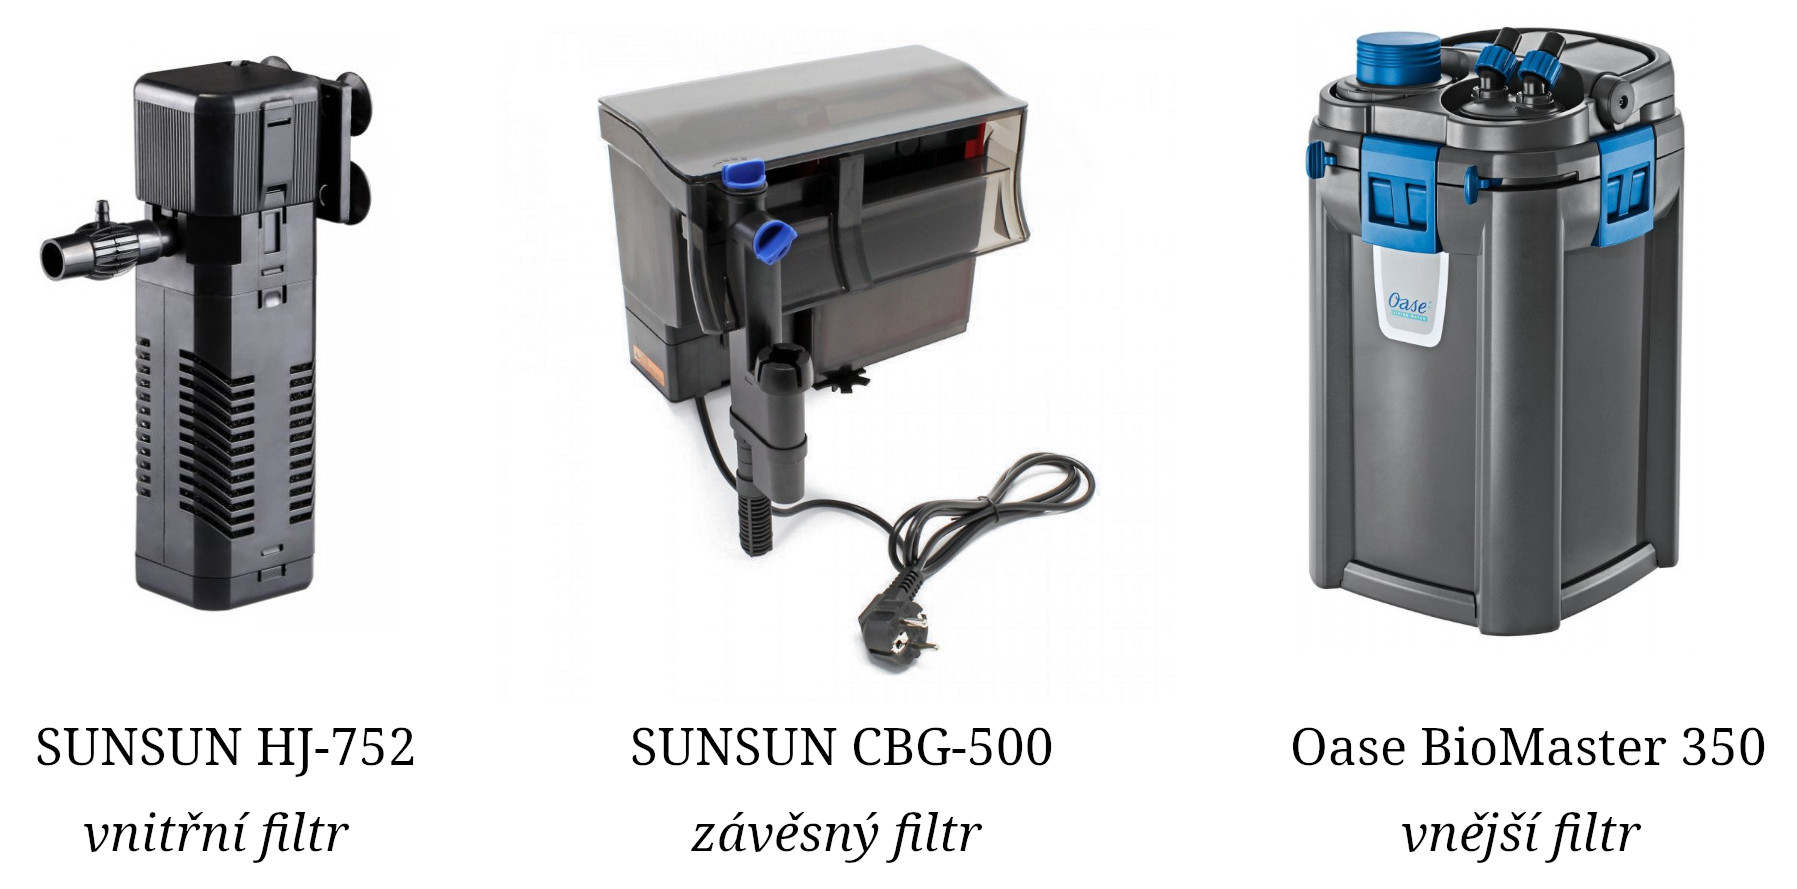
\includegraphics[width=\textwidth]{obrazky/filtry/filtry.jpg}
            \caption{Příklad různých typů filtrů. Převzato z~\cite{eshop-rostlinna-akvaria}.}
            \label{fig:filtry-srovnani}
        \end{figure}

    \subsection{Osvětlení}
        Funkce osvětlení akvária je dvojí. Jednak jde o~estetický dojem z~pohledu pozorovatele, kdy vhodné nasvícení přidává akváriu na atraktivitě. Druhak se osvětlení snaží nasimulovat osazenstvu akvária přirozené životní podmínky, aby celý ekosystém mohl fungovat.

        Hlavními parametry při výběru svítidla jsou jeho \textbf{intenzita}, \textbf{spektální charakteristika} a \textbf{spotřeba}. 
        
        Příliš intenzivní světlo zvyšuje riziko nežádoucí tvorby řas a pro ryby může být stresovým faktorem, nízká intenzita zase může způsobit špatný růst rostlin~\cite{KejzlarRadim2022Ařpa}. Na internetu existuje mnoho návodů a rad na stanovení správné intenzity, ale protože zde hraje roli spousta dalších parametrů jako např. výška hladiny nebo konkrétní typ rostlin, je vhodné tyto hodnoty brát pouze jako orientační a intenzitu osvětlení upravit během provozu podle potřeby. Výpočet se také liší pro jednotlivé typy svítidel. 

        Spektrum světla hraje roli hned z~několika důvodů. Rostliny pro tvorbu chlorofylu a následnou fotosyntézu potřebují světlo zejména vlnových délek \qty{440}{nm} (modrá barva) a \qty{660}{nm} (červená barva)~\cite{eshop-ledsolution-svetlo}, pokud by zvolené osvětlení tyto vlnové délky neobsahovalo, nemohou rostliny správně fungovat. Akvárium osvětlené pouze těmito dvěma barvami by ale nevypadalo vizuálně dobře, proto se využívá také širokospektrální bílé světlo, které svým spektrem odpovídá co nejlépe dennímu světlu. 
        Specializovaná svítidla pak nabízejí možnost napodobit světelné spektrum různých vodních prostředí a přizpůsobit se tak i rostlinám a živočichům žijícím ve velkých hloubkách. 

 
        \begin{figure}[h!]
            \centering
            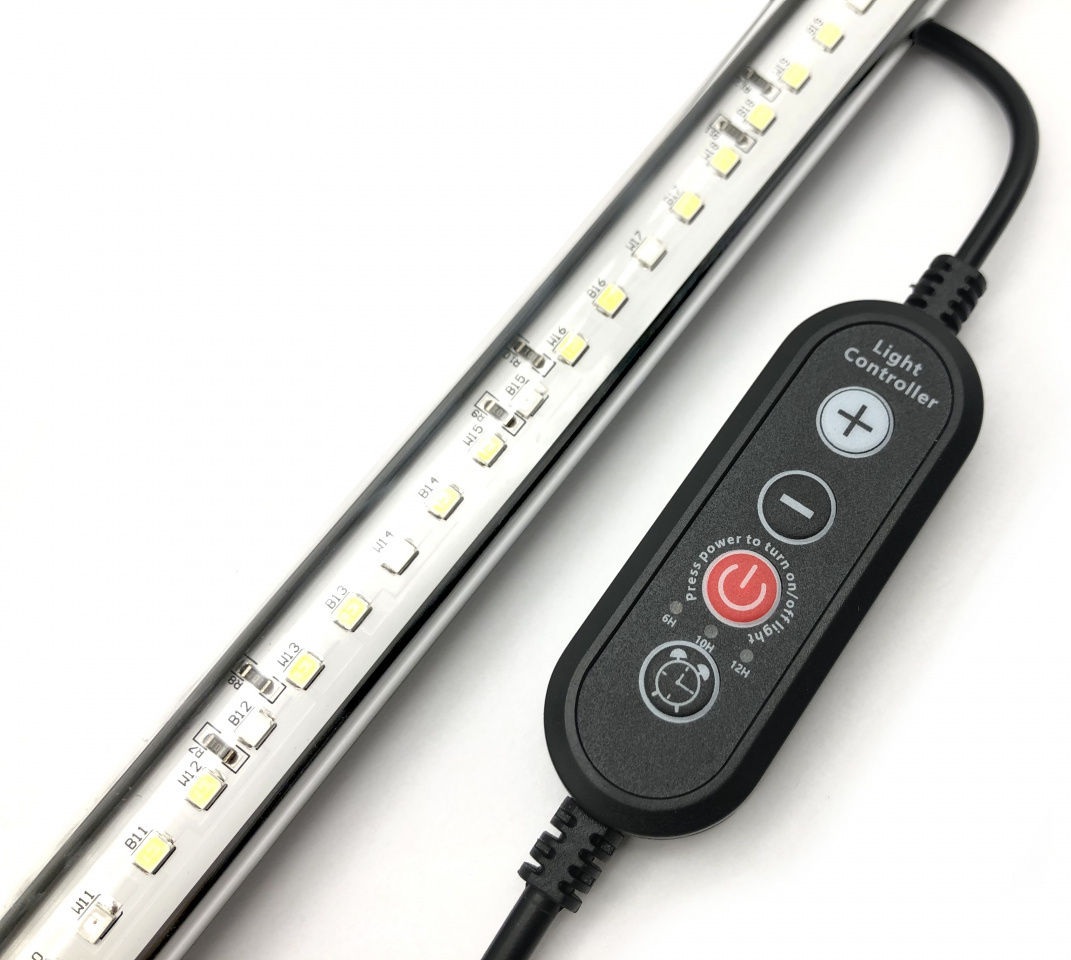
\includegraphics[width=0.5\textwidth]{obrazky/osvetleni/stmivac.jpg}
            \caption{Trubice s~\acs{led} páskem a manuální stmívač a časovač. Převzato z~\cite{eshop-rostlinna-akvaria}.}
            \label{fig:obrazky-osvetleni-stmivac-jpg}
        \end{figure}

        Na trhu jsou v~současné době tři typy akvaristických světel: \textbf{zářivky}, \textbf{výbojky}  a \textbf{\acs{led} svítidla}~\cite{eshop-rostlinna-akvaria-svetlo}. Zářivky jsou považovány za dnes již nepříliš moderní řešení a bývají nahrazovány \acs{led} svítidly, ty se vyznačují lepší účinností (tedy nižší spotřebou energie při stejné intenzitě světla), delší životností a širší paletou barev. U~zářivek také nebylo možné plynule regulovat intenzitu, jako je tomu u~\acs{led}, a dosáhnout tak např. postupného rozsvícení nebo zhasnutí světla simulujícího východ a západ slunce. Skoková změna při zapnutí nebo vypnutí světla je pro ryby také zbytečným stresovým faktorem~\cite{MusilLibor2018Isps}. Co se týče výbojek, ty nacházejí uplatňení zejména pro hluboké nádrže, protože jejich světlo je bodové a intenzita dostačující k~prosvícení velkého objemu vody, spotřeba energie je ale v~porovnání s~\acs{led} vysoká, takže pokud to není nezbytně nutné, je lepší se jim vyhnout.   

        Typické domácí akvárium je osvětleno jedním nebo několika samostatně stmivatelnými \acs{led} svítidly, a to buďto v~podobě \acs{led} pásků nalepených na hliníkovém profilu anebo hotového svítidla, ve kterém jsou čipy s~\acs{led} zabudovány napevno. Stmívání je nastavováno buď ručně anebo za pomoci mobilní aplikace dodané výrobcem stmívače. Příklad běžně dostupného výrobku lze vidět na obr.~\ref{fig:obrazky-osvetleni-stmivac-jpg}.

    \subsection{Ohřev}
        Většina okrasných sladkovodních ryb běžně chovaných akvaristy pochází z~tropických krajů a vyžaduje teplotu vody v~rozmezí 22 -- \qty{26}{\degreeCelsius}~\cite{slavotinek2014}, to je o~něco málo vyšší teplota než bývá v~domácnosti typická a proto je nutné zajistit akváriu možnost dodatečného ohřevu. Nejčastějsím řešením je ponorné topné těleso na odporové bázi s~vlastní termostatovou regulací, viz obr.~\ref{fig:obrazky-topeni-topitko-jpg}.

        \begin{figure}[h!]
            \centering
            \begin{tikzpicture}
                % Include the image
                \node[anchor=south west,inner sep=0] (image) at (0,0) {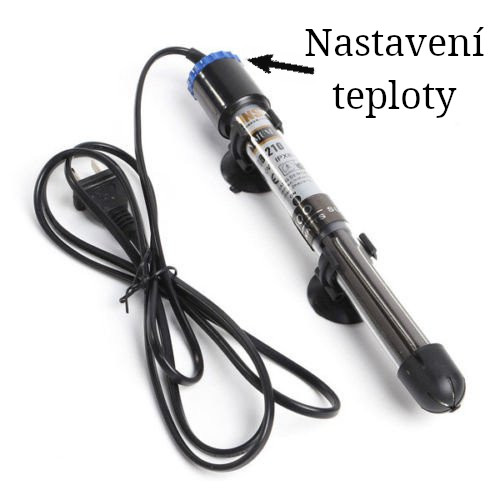
\includegraphics[width=0.5\textwidth]{obrazky/topeni/topitko.jpg}};

                \node (termostat) at (3.8,6.5) {};
                \node[align=center] (napis) at (6,6.5) {Nastavení\\teploty};
                \draw[->] (napis) -- (termostat);
                
            \end{tikzpicture}

            \caption{SUNSUN topítko 100W s~termostatem. Převzato z~\cite{eshop-rostlinna-akvaria}.}
            \label{fig:obrazky-topeni-topitko-jpg}
        \end{figure}
        
        Z~principu fungování termostatu vyplývá, že výsledná teplota vody není v~čase konstantní, ale osciluje okolo nastavené hodnoty. Rozsah kolísání teploty je pak závislý na hysterezi termostatu, obecně lze říci, že to může být i několik stupňů. Pro většinu aplikací to není velký problém, ale některé druhy ryb mohou být na změny teploty náchylnější, v~takovém případě je potřeba buďto vybrat topítko takové, kde výrobce rozsah teplot uvádí, anebo zvolit jiný způsob regulace. 

    \subsection{Monitorování}
    \label{sec:monitorovani}
        Jak již vyplynulo z~úvodních kapitol, v~akváriu probíhá celá řada procesů ovlivňujících jeho stav. Klíčem k~vytvoření prosperujícího akvária je dosažení rovnováhy a stability mezi nimi za pomoci vhodně nastavené akvarijní techniky. Nejen u~začínajících akvaristů se mohou vyskytnout problémy s~růstem rostlin, zdravím ryb nebo třeba výskytem řasy. Odhalit příčiny těchto problémů může být mnohdy obtížné, ovzláště pokud není k~dispozici dostatečné množství informací o~tom, co se v~akváriu děje. 
        
        Existuje několik veličin, které úzce souvisí s~procesy v~akváriu a které je možné také poměrně jednoduše sledovat. Na trhu je celá řada produktů sloužících k~tomuto účelu. Většinou je na výběr možnost analogového nebo čistě mechanického přístroje případně samostatného digitálního čidla, existují ale také komplexní řešení, těm se dále věnuje kapitola  \ref{lab:kapitola-komplexni-reseni}. 

        \subsubsection{Teplota}
            Umístěním teploměru (ať už v~analogové nebo digitální podobě) do akvária je možné zkontrolovat správné nastavení topného tělesa a následně provést jeho úpravu. Také lze včas získat informaci o~jeho případné poruše a nebo třeba jen nedostatečném výkonu. 
        \subsubsection{\acs{ph} a CO\(\mathbf{_{2}}\)}
            Hodnota \acs{ph} popisuje kyselost resp. zásaditost měřeného vodného roztoku. Běžně se používá logaritmická stupnice s~hodnotami 0 až 14, přičemž zcela neutrální voda má \acs{ph} rovno 7, menší hodnoty mají roztoky kyselé a větší než 7 pak roztoky zásadité.  Obecně lze říci, že pro ryby je vyhovující \acs{ph} v~rozsahu 6 až 8~\cite{slavotinek2014}. 

            Důležitým parametrem vody z~pohledu rostlin a ryb je koncentrace \acs{co2}. Přirozeně platí, že rostliny \acs{co2} spotřebovávají při fotosyntéze a jistá koncentrace je tedy nutná pro jejich prosperitu, naopak příliš vysoká koncentrace může být nebezpečná pro ryby, kterým (obdobně jako např. lidem) komplikuje dýchání. Obsah \acs{co2} ve vodě je obtížné přímo měřit, jeho měnící se koncentrace má ale vliv právě na hodnoty \acs{ph}, s~rostoucí koncentrací \acs{co2} se \acs{ph} vody snižuje a obráceně~\cite{DvorakJan2014RPpa,KejzlarRadim2022Ařpa}. 

            K~měření \acs{ph} vody se používají různé chemické testy (kapkové testy, testovací papírky), které je možné zakoupit v~chovatelských potřebách. Z~pohledu automatizace je mnohem zajímavějším řešením \acs{ph} sonda, která umožňuje nepřetržité měření této veličiny a případnou okamžitou regulaci dávkování \acs{co2}.

             
    \subsection{Dostupná komplexní řešení}
    \label{lab:kapitola-komplexni-reseni}
        Tato sekce se věnuje porovnání několika nejznámějších systémů v~oblasti automatizace akvárií. Je důležité připomenout, že ve všech oblastech elektrotechniky dochází k~rychlému rozvoji a každý rok se na trhu objevují nové produkty se stále lepšími parametry a nižší cenou. Informace uvedené v~této kapitole, a to zejména cenové údaje, se mohou velmi rychle stát neaktuálními a jsou tedy relevantní pouze v~době vzniku této práce.

        Při tvorbě této kapitoly byly jako zdroj informací použity jednak oficiální materiály výrobců, ty ovšem samozřejmě obsahují vždy pouze pozitivní informace, dále pak různé uživatelské recenze na platformě YouTube popř. diskuzních fórech, nejedná se o~zcela seriózní zdroje a proto je nutné také informace z~této kapitoly brát s~rezervou. 

        % TODO: Tento obr. až v GHL kapitole - nebudu, NEBUDU TO DĚLAT !!
        \begin{figure}[h!]
            \centering
            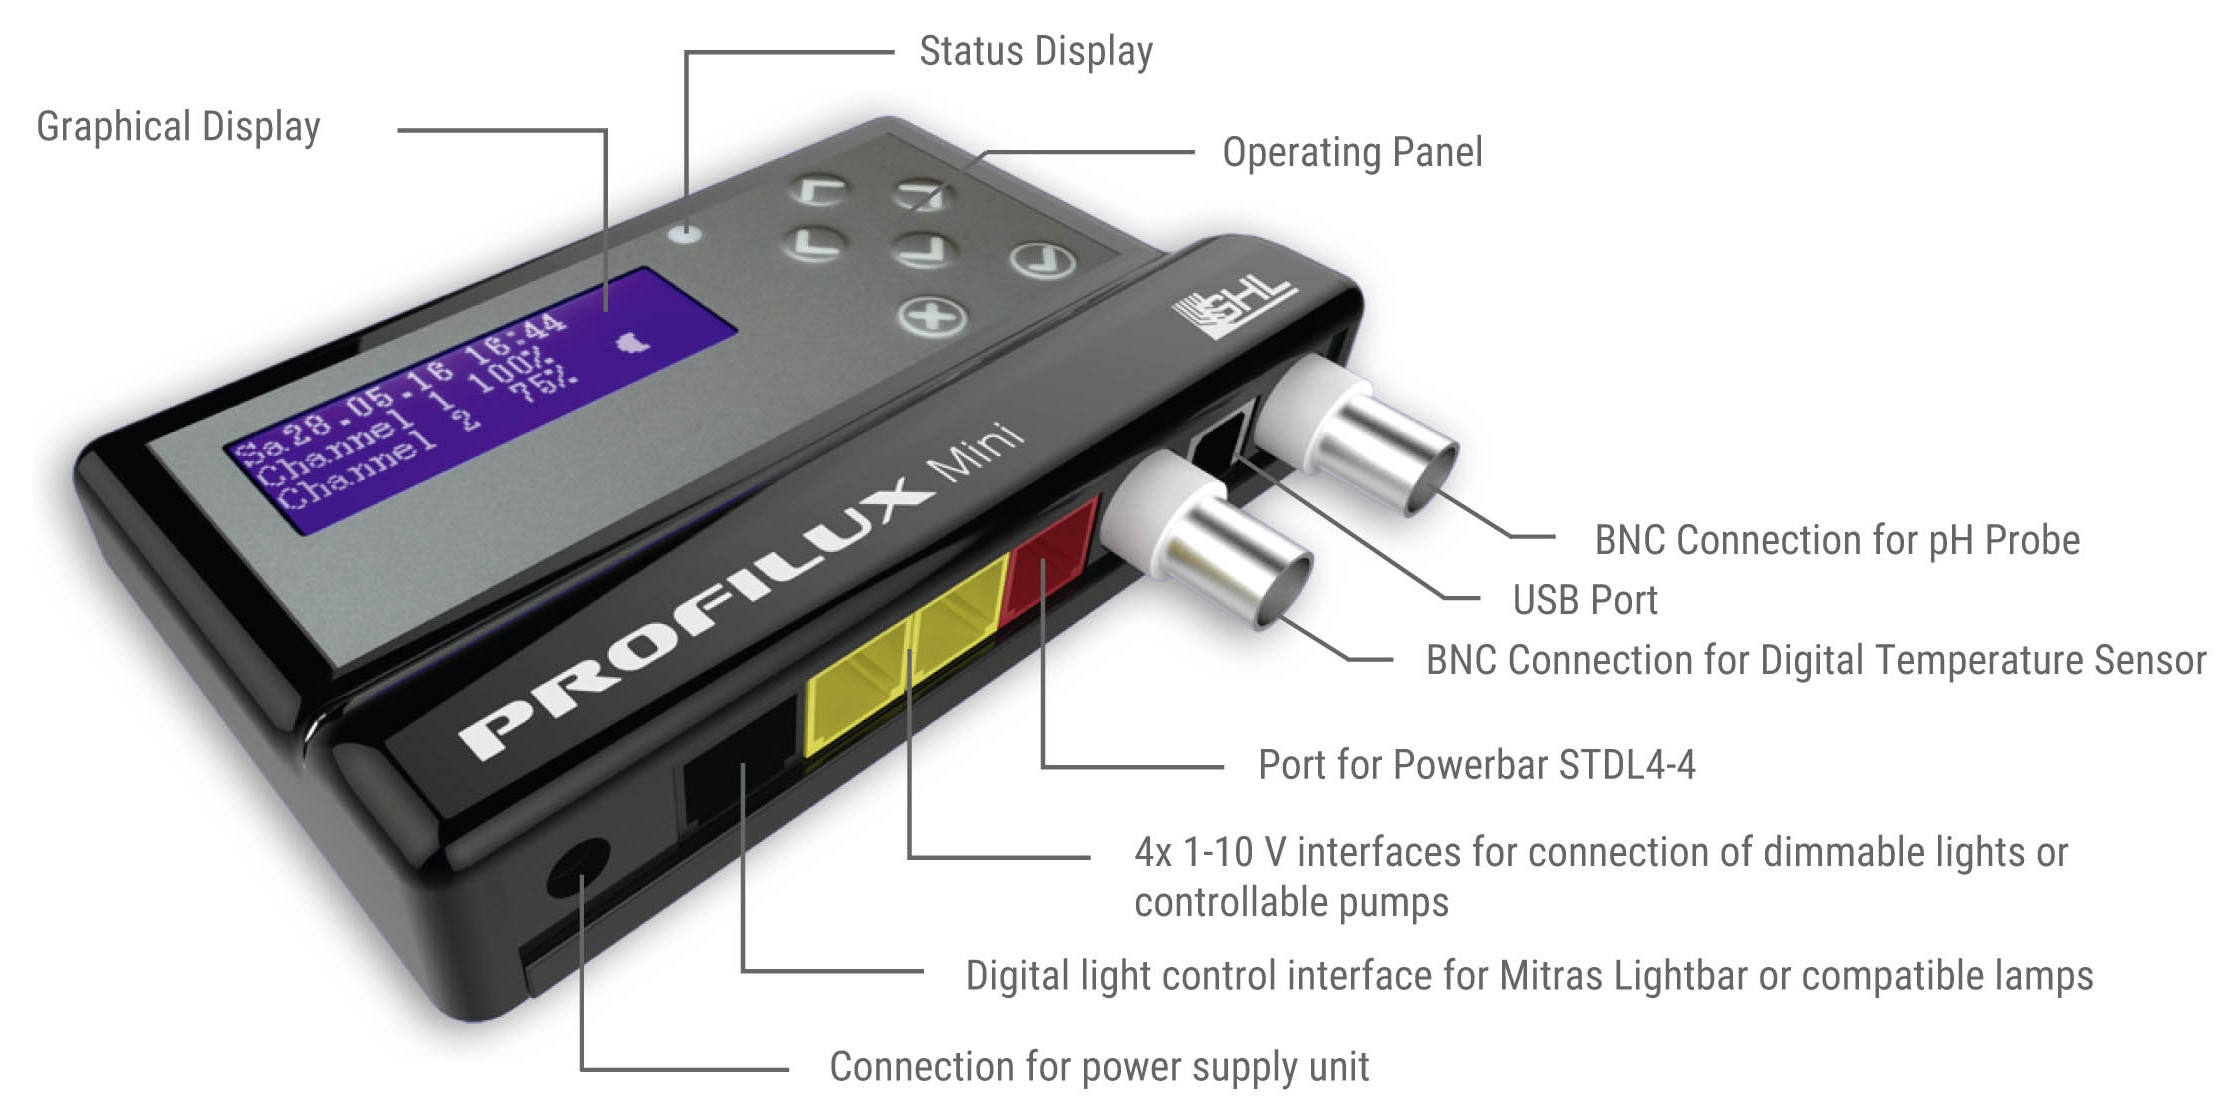
\includegraphics[width=0.9\textwidth]{obrazky/trh/GHL-ProfiLux-Mini.jpg}
            \caption{GHL ProfiLux Mini, nejmenší dostupný kontrolér této firmy. Převzato z~\cite{ghl-profilux}.}
            \label{fig:obrazky-trh-GHL-ProfiLux-Mini-jpg}
        \end{figure}
        \subsubsection{GHL -- ProfiLux}
            Německá firma GHL se v~oblasti akvaristiky pohybuje již přes 20 let a patří nepochybně ke špičce na trhu z~hlediska komplexity a spolehlivosti. Základem jejich systému ProfiLux je kontrolér (např. nejmenší varianta viz obr.~\ref{fig:obrazky-trh-GHL-ProfiLux-Mini-jpg}), který je možné konfigurovat z~PC za pomocí kabelu anebo vzdáleně s~použitím aplikace nebo webového rozhraní. Ke kontroléru lze připojit celou řadu periferíí z~portfolia firmy, jedná se o~různé typy senzorů, dávkovače (pro úpravu parametrů vody), pumpy nebo řiditelný prodlužovací přívod pro síťové zásuvky (laicky řečeno \uv{chytrá prodlužovačka}). Společnost si zakládá na opravdu vysoké kvalitě a přesnosti svých výrobků, což se ale odráží také na jejich ceně. 

            Na výběr je z~několika variant systému, přičemž ty nejdražší dokážou obsloužit i opravdu rozsáhlé a náročné akvaristické instalace. Cena nejlevnějšího základního setu je přibližně od \qty{10000}{Kč}~\cite{ghl-profilux,eshop-ghl-profilux-sets}.

            
        \subsubsection{Neptune Systems -- Apex}
            Systém Apex je nepochybně další ze světových leaderů v~této oblasti. Opět je k~dispozici několik variant systému podle požadavků a finančních možností uživatele a systém je také velmi modulární. Stejně jako firma GHL, i Neptune Systems je na trhu více než 20 let a jedná se tedy o~léty ověřenou značku. Architektura systému je podobná a kromě samotného kontroléru je opět v~nabídce celá řada kompatibilních periferií. Dle uživatelských recenzí je konfigurace systému oproti GHL výrazně jednodušší a není nutná znalost programování, navíc systém už od výroby obsahuje přednastavené nejčastější scénáře použití.

            \begin{figure}[h!]
                \centering
                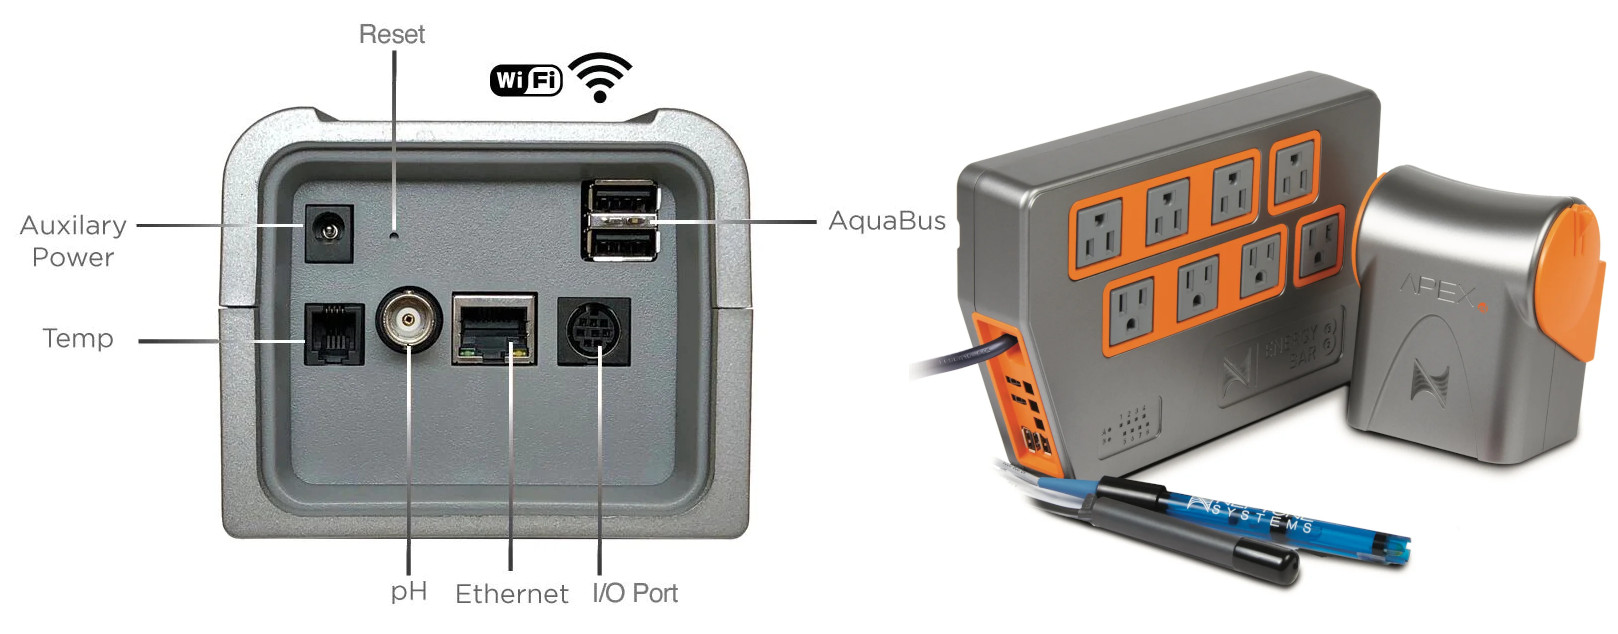
\includegraphics[width=0.8\textwidth]{obrazky/trh/apex-el.jpg}
                \caption{Neptune Systems Apex EL, základní set. Převzato z~\cite{eshop-neptune-systems-apex}.}
                \label{fig:obrazky-trh-apex-el}
            \end{figure}
            
            Cena opět závisí na množství zakoupených modulů, základní set s~podobnou výbavou jako u~GHL je k~dispozici přibližně od \qty{12000}{Kč}~\cite{neptune-systems-why-apex,eshop-neptune-systems-apex}.

        \subsubsection{CoralVue -- HYDROS}
            Firma CoralVue se svým systémem HYDROS je na trhu oproti svým konkurentům relativně krátce, přibližně 3 roky, svým originálním přístupem a cenově dostupným řešením si ale své zákazníky našla rychle. Systém je svou architekturou ještě více modulární než jeho konkurenti, umožňuje v~rámci jedné aplikace spojit i více kontrolérů, které mezi sebou komunikují. Dokonce v~případě poruchy hlavního kontroléru dokáže jeho roli převzít jiný připojený kontrolér a systém tak zůstane dále v~provozu. 
            
            Kromě bezdrátově řízeného modulu se čtyřmi síťovými zásuvkami nově firma nabízí také modul Control XP8, který krom zásuvek obsahuje i vlastní kontrolér, může tak fungovat zcela samostatně, stále však umožňuje také drátové spojení s~dalšími kontroléry nebo bezdrátové připojení k~dalším zásuvkám. Toto může sloužit jako jednoduché univerzální řešení pro menší akvária s~možností budoucího rozšíření. 

            \begin{figure}[h!]
                \centering
                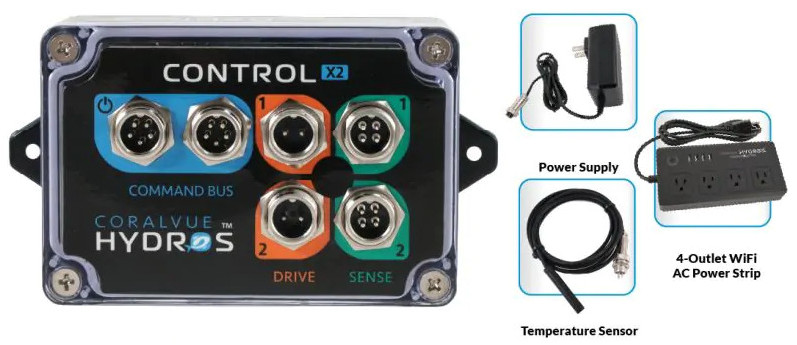
\includegraphics[width=\textwidth]{obrazky/trh/hydros-x2-starter-pack.jpg}
                \caption{CoralVue HYDROS Control X2 Starter pack. Převzato z~\cite{eshop-coralvue-hydros}.}
                \label{fig:obrazky-trh-hydros-x2-starter-pack-jpg}
            \end{figure}
            
            Základní minimální sada je dostupná již od přibližně \qty{4500}{Kč}, aby byla ale výbava stejná jako u~výše zmíněných konkurentů je potřeba dokoupit ještě \acs{ph} sondu za přibližně \qty{800}{Kč}~\cite{coralvuehydros,eshop-coralvue-hydros}.
            
        \subsubsection{Seneye}
            Společnost Seneye nenabízí komplexní řešení pro automatizaci, ale i přesto jsou její produkty zajímavé a pro mnoho akvaristů mohou být skutečně užitečné. Místo pokročilého ovládání akvarijní techniky se výrobky zaměřují pouze na monitorování parametrů vody (popř. dalších veličin), důraz je kladen na maximální jednoduchost použití. 
            
            \begin{figure}[h!]
                \centering
                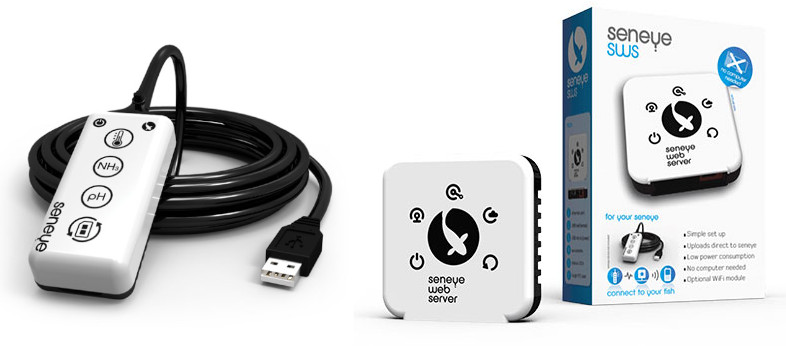
\includegraphics[width=0.6\textwidth]{obrazky/trh/seneye-home.jpg}
                \caption{Seneye Home a Seneye Web Server. Převzato z~\cite{seneye-home}.}
                \label{fig:obrazky-trh-seneye-home-jpg}
            \end{figure}

            Vnitřním sladkovodním akváriím je věnována řada Seneye Home a veškeré monitorování je zajištěno jedním malým zařízením, které uživatel přímo ponoří do vody a pomocí kabelu připojí k~počítači ze kterého se zařízení napájí a zároveň do něj odesílá data. Alternativně lze přikoupit také krabičku, která slouží jako webserver, do ní se zařízení připojí namísto počítače a data jsou rovnou zálohována do cloudu, odkud jsou uživateli dostupná v~mobilní aplikaci. Ukázkové foto je na obr.~\ref{fig:obrazky-trh-seneye-home-jpg}.

            Zařízení monitoruje teplotu, \acs{ph}, úroveň škodlivého amoniaku, osvětlení a hladinu vody. Umožňuje také odesílat oznámení při překročení nastavené meze některého z~parametrů.

            Cena samotného monitorovacího zařízení je přibližně \qty{3000}{Kč} a podobná je také cena zmíněného webserveru. Pro automatické monitorování se zálohou na cloud je tedy potřeba počítat s~investicí okolo \qty{6000}{Kč}~\cite{seneye-home}.
            


        









\chapter{Systémový návrh}

Tato část práce popisuje proces návrhu vlastního zařízení, který by měl být výstupem této práce. Věnuje se konkretizaci požadavků na zařízení a koncepčního návrhu na systémové úrovni, který je zde podpořen blokovým schématem. Po celou dobu tvorby zařízení bude kladen důraz na požadavky stanovené v této kapitole a na jejich základě budou tvořena vhodná technická řešení.  Detailně se jednotlivým blokům a jejich návrhu věnuje kapitola~\ref{kap:navrh-dilnich-bloku}.

\section{Požadavky}
\label{sec:pozadavky}
    Cílem je vytvořit zařízení, které umožní co nejvíce automatizovat provoz akvária. Hlavním aspektem by měla být jednoduchost použití pro koncového uživatele, vše by mělo být nanejvýš intuitivní a přehledné. Zařízení musí mít možnost připojení k~internetu prostřednictvím sítě Wi-Fi, uživatel tak bude moci zařízení konfigurovat a sledovat z~libovolného místa za pomoci webové stránky popř. mobilní aplikace.

    Požadavky jednotlivých akvaristů se mohou lišit a zároveň se v~čase měnit. Vytvoření dokonalého a všestaranného zařízení, které vyhoví všem účelům použití není v~časových ani finančních možnostech bakalářské práce, proto byl stanoven požadavek, aby bylo zařízení co nejvíce modulární a rozšiřitelné. Musí být zvolena taková architektura, aby bylo možné v~budoucnu přidat další funkce a periferie bez nutnosti modifikovat stávající hardware.

    Výstupem bakalářské práce by mělo být zařízení schopné monitorovat některé akvaristické veličiny a na základě jejich hodnoty informovat uživatele a ovládat akvárium. Zařízení bude přímo řídit \acs{led} páskové osvětlení na \qty{12}{V} a spínat popř. vypínat již existující akvaristické přístroje pracující se síťovým napětím \qty{230}{V}.  

    Jelikož modulární architektura bude nepochybně vyžadovat použití více než jednoho mikrokontroléru a tedy také více různých firmwarů, je potřeba zajistit jejich vzájemnou kompatibilitu a stabilitu celého systému. Veškerý firmware tak musí být verzovaný a po připojení nové periferie musí řídicí jednotka rozpoznat, o~jakou periferii se jedná. V~případě připojení nekompatibilní periferie (např. z~důvodu zastaralého firmwaru řídicí jednotky) musí být uživatel upozorněn a nesmí být nijak narušena funkce zbytku systému. Aby bylo možné těmto situacím předejít, musí mít řídicí jednotka možnost vzdálené aktualizace firmwaru.
\section{Koncepční schéma}












\section{Řídící jednotka}

\chapter{Obecný modul periferie}
\label{sec:modul-periferie}
    Díky zvolené koncepci systému je možné za periferii považovat jakékoliv zařízení schopné obousměrně komunikovat po navržené sběrnici. Není vyloučeno, aby byla každá periferie navržena zcela odlišně na základě svých vlastních požadavků na výkon, počet pinů nebo dostupná rozhraní daného MCU. Hlavní výhodou této koncepce je to, že periferie mohou být vyvíjeny postupně a přidávány do již funkčního a odladěného systému bez nutnosti modifikovat stávájící hardware. V~případě chyby v~návrhu periferie je také oprava méně náročná, než by tomu bylo v~případě zabudování veškeré funkcionality přímo do řídicí jednotky. 

    Nicméně pokud by byl pro každou periferii zvolen zcela jiný mikrokontrolér a vytvořen vlastní návrh DPS, vývoj více periferií by byl zbytečně drahý a časově náročný. Proto byl zvolen koncept \uv{obecného modulu periferie}, tedy jedné DPS s~konkrétním mikrokontrolérem zajišťující připojení ke komunikačního rozhraní, napájení periferie a rozhraní pro programování. Kromě toho budou na DPS dvě dutinkové lišty, do kterých bude možné vsadit druhou DPS (popř. během vývoje pouze prototypovací desku) ve funkci dceřinné desky (ang. daughterboard). Vložená deska pak bude obsahovat obvody nutné přímo pro danou konkrétní periferii.
    
    \section{Mikrokontrolér}

        Kritéria pro výběr mikrokontroléru byla následující:
        \begin{itemize}
            \item Musí nutně splňovat:
            \begin{itemize}
                \item CAN periferie -- pro komunikaci po sběrnici 
                \item PWM výstup -- řízení LED, popř. jiné
                \item ADC -- pro práci s analogovými sensory
                \item Nízká cena 
            \end{itemize}
            \item Je výhodou:
            \begin{itemize}
                \item Dobrá dokumentace, komunita uživatelů
                \item Zkušenost autora s~danou platformou
                \item Další periferie (\acs{i2c}, SPI, ...)
            \end{itemize}
        \end{itemize}

        Na základě těchto kritérií byl vybrán mikrokontrolér \textbf{PIC18F26Q83} od firmy Microchip, ten splňuje všechna kritéria a disponuje také množstvím dalších periferií, které by mohly být v~budoucnu užitečné~\cite{PIC18F26Q83}.

    \section{Návrh zapojení a tvorba DPS}
        Celé schéma pro obecný modul periferie se nachází v příloze~\ref{priloha:schema-modul-periferii}. Návrh zapojení lze rozdělit na tři části. V prvním kroku je zapojen mikrokontrolér tak, aby byly opět splněny všechny požadavky výrobce. Mikrokontroléry řady PIC se vyznačují značnou jednoduchostí použití a ke správnému chodu jim stačí jen minimum dalších součástek. V případě PIC18F26Q83 postačí připojit blokovací kondenzátor (C6) na napájení (pin VCC) a přivést kladné napětí na resetovací pin (MCLR). MCU je dále doplněn resetovacím tlačítkem pro pohodlnější práci při vývoji a testování firmwaru a regulátorem napětí (U1) s výstupem \qty{3.3}{V}. 

        Ve druhém kroku je přidána dvojice D-sub konektorů a CAN řadič ATA6561 obdobně jako u řídicí jednotky popsané v kapitole \ref{sec:ridici-jednotka-schema-a-dps}. Na závěr jsou všechny dosud nevyužité piny vyvedeny na konektor (dutinkovou lištu), aby byly jednoduše dostupné pro připojenou dceřinnou desku. Pro napájení výkonově náročnejších periferií (např. ovladač LED osvětlení) jsou zvlášť vyvedeny ještě dvě trojice pinů připojené na \qty{24}{V} a zem (GND).

        \subsubsection{Tvorba DPS}
        Hlavním cílem bylo vytvořit DPS co nejmenší. Jedná se o samostatné moduly, kterých bude v systému zapojeno několik a pro manipulaci a rozmístění modulů okolo akvária je menší rozměr výhodou. Hlavní limitací v této snaze není počet součástek, ale spíše rozměry mechanických prvků, zejména konektorů D-sub. Na obr.~\ref{fig:modul-periferie-dps} je vidět výsledný návrh DPS s osazenými součástkami a dosaženými rozměry. Je zřejmé že jiným rozložením dutinkových lišt by se návrh dal ještě drobně zmenšit, ale je potřeba ponechat jistou flexibilitu pro tvorbu dceřinných desek.

        \begin{figure}[!ht]
            \centering
            \begin{tikzpicture}
                % Include the image
                \node[anchor=south west,inner sep=0] (image) at (0,0) {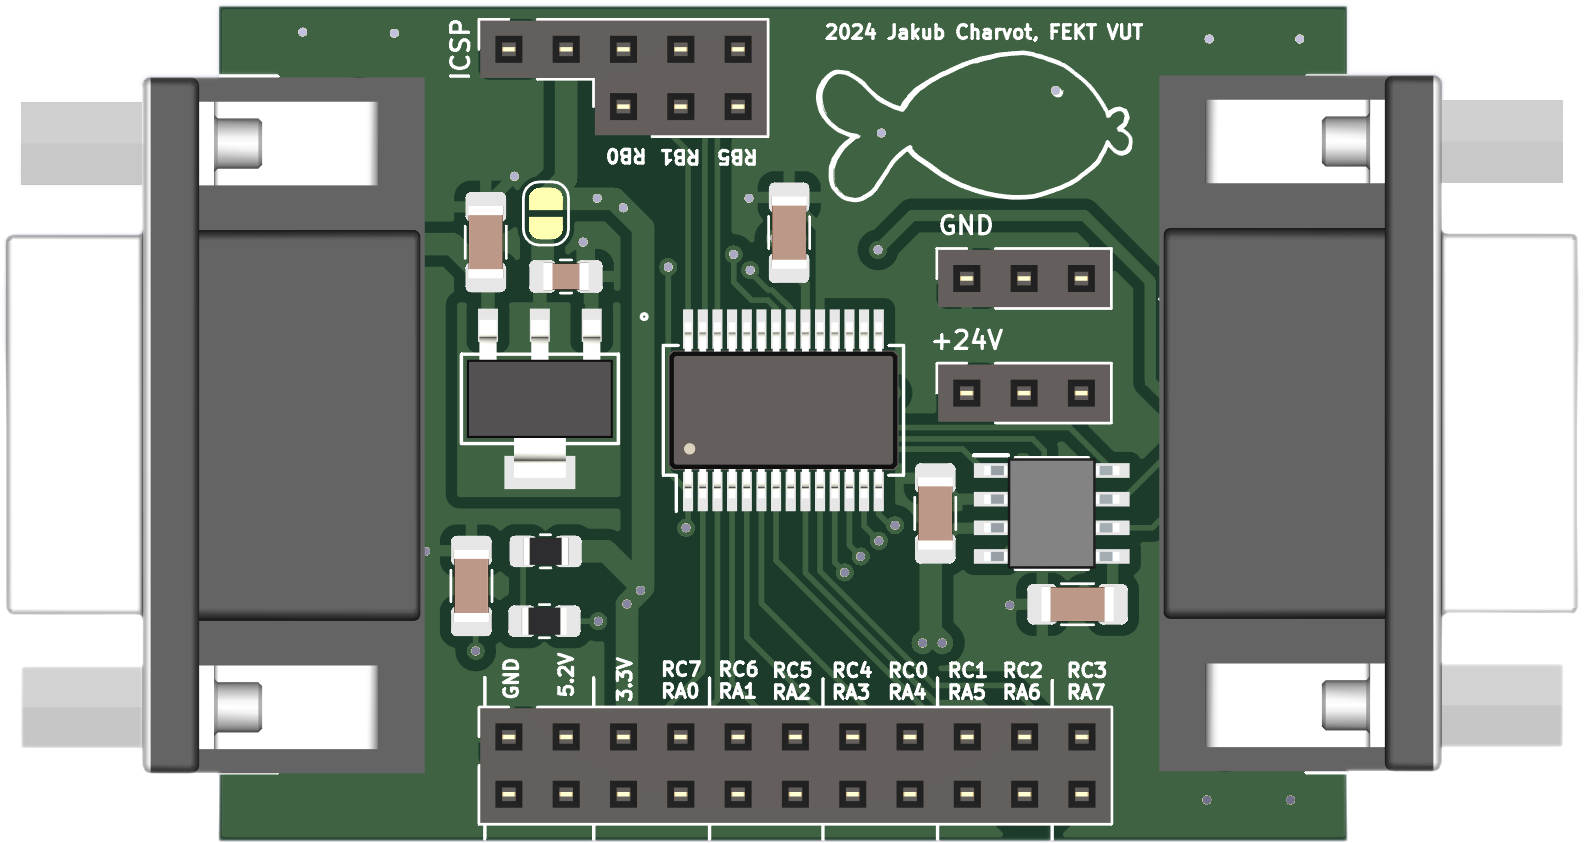
\includegraphics[width=0.8\textwidth]{obrazky/dps/peripherial-module-3d-top.png}};
                
                \draw[dashed] (10.1,0.04) -- (12.5,0.04);
                \draw[<->,thick] (12.5,0.04) -- (12.5,6.34);
                \draw[dashed] (12.5,6.34) -- (10.1,6.34);
                \node[anchor=west] at (12.5,3.15)  {\qty{36}{mm}};

                \draw[dashed] (1.12,0.64) -- (1.12,-0.5);
                \draw[<->,thick] (1.12,-0.6) -- (10.9,-0.6);
                \draw[dashed] (10.9,-0.6) -- (10.9,0.64);
                \node[anchor=south] at (6,-0.6)  {\qty{57}{mm}};
            \end{tikzpicture}
            \caption{Vizualizace DPS obecného modulu periferie.}
            \label{fig:modul-periferie-dps}
        \end{figure}

        Co se týče rozložení vrstev, byla opět použita čtyřvrstvá deska se strejnou strukturou jako je na obr.~\ref{fig:ridici-jednotka-stackup-dps} pro DPS řídicí jednotky. Celý návrh DPS se nachází v příloze TODO.





\chapter{Volba a návrh periferií}
    Tato kapitola se již věnuje návrhu konkrétních periferií, tedy jednotlivých senzorů a akčních členů. Po technické stránce jsou všechny zmíněné moduly nadstavbou pro \uv{obecný modul periferie} popsaný detailně v předešlé kapitole. Jelikož je celý systém modulární, je pravděpodobné, že postupem času bude dále rozšiřován o nové typy periferií a i v současné chvíli je jich v plánu více, než je v možnostech této práce. Pro lepší přehlednost se v tab.~\ref{tab:prehled-periferii} nachází přehled všech realizovaných i v tuto chvíli pouze plánovaných periferií.

    \begin{table}[h]
        \centering
        \caption{Přehled periferií.}
        \label{tab:prehled-periferii}
        \begin{tabular}{|l|l|l|l|l|}
            \hline
            Název & Typ & Napájení & Funkce & Realizováno \\ \hline\hline
            Sensor teploty  & S & \qty{5}{V}    & Teplota vody                       & Ano, kap.~\ref{sec:perif-sensor-teploty}  \\ \hline
            Sensor hladiny  & S & \qty{5}{V}    & Výška hladiny (spojitě + skokově)  & Ano, kap.~\ref{sec:perif-sensor-hladina}  \\ \hline
            \acs{led} osvětlení   & A & \qty{24}{V}   & Intenzita osvětlení                & Ano, kap.~\ref{sec:perif-led-osvetleni}  \\ \hline
            Sensor \acs{ph}       & S & \qty{5}{V}    & \acs{ph} vody                            & Ano, kap.~\ref{sec:perif-sensor-ph}  \\ \hline
            Topné těleso    & A & \qty{230}{V}  & Ohřev vody                         & Ano, kap.~\ref{sec:perif-230v}  \\ \hline
            Filtr vody      & A & \qty{230}{V}  & Filtrace vody                      & Ano, kap.~\ref{sec:perif-230v}  \\ \hline
            Krmítko         & A & \qty{24}{V}   & Dávkování krmiva                   & Ne  \\ \hline
            Sensor průtoku  & S & -             & Voda tekoucí filtrem               & Ne  \\ \hline
                            % & S &  &  & A  \\ \hline
                            %     & S &  &  & A  \\ \hline
                            %     & S &  &  & A  \\ \hline
                            %     & S &  &  & A  \\ \hline
                            %     & S &  &  & A  \\ \hline
                            %     & S &  &  & A  \\ \hline
                            %     & S &  &  & A  \\ \hline
                            %     & S &  &  & A  \\ \hline
                            %     & S &  &  & A  \\ \hline
            \end{tabular}
            \begin{tabular}{c}
                S = sensor, A = akční člen \\
            \end{tabular}
   
    \end{table}

\section{Senzor teploty}
\label{sec:perif-sensor-teploty}
    Cílem tohoto modulu je kontinuálně měřit teplotu vody a naměřená data poskytovat řidicí jednotce skrze sběrnici \acs{can}. Při volbě konkrétního teplotního čidla je potřeba vzít v potaz několik faktorů:
    \begin{itemize}
        \item Přesnost a rozsah
        \item Časová stálost
        \item Složitost implementace 
        \item Pouzdro určené pro ponoření do vody
        \item Cena
    \end{itemize}

    \subsection{Metody měření teploty}
        Nejčastěji používanými součástkami určenými k měření teploty jsou nepochybně termistory a termočlánky~\cite{allaboutcircuits2023tempsensors}. Termistor je rezistor vytvořen z materiálu, který mění svůj odpor v závislosti na teplotě přičemž rozlišujeme dva základní typy termistorů podle toho, zda s rostoucí teplotou jejich odpor roste (PTC termistor) anebo klesá (NTC termistor). U obou typů lze obecně říci, že závisost odporu na teplotě je značně nelineární, pro zjištění přesné teploty je tedy potřeba buďto měřená data dále zpracovat (např. mikrokontrolérem) anebo využít speciální integrovaný obvod, který výstup z připojeného termistoru linearizuje a dále propaguje buďto v analogové nebo i digitální podobě. Jelikož odpor termistoru a stejně tak i dalších součástek, potřebných k jeho zapojení, má jistou výrobní toleranci, je vhodné sensor před použitím kalibrovat.

        Princip termočlánku je odlišný, jedná se o vodivé spojení dvou kovů na kterém díky Seebeckově jevu vzniká termoelektrické napětí. Velikost tohoto napětí je daná použitými materiály a je také teplotně závislá. V praxi se používá nejčastěji několik dvojic materiálů, které svými vlastnostmi a cenou nejvíce vyhovují běžným požadavkům, ty pak získaly také své označení jako termočlánky typu J, K, T nebo E (typů existuje více, uvedeny jsou nejčastěji používané~\cite{TechieScience_Thermocouples}). Termočlánky pracují oproti ostatním senzorům s výrazně větším rozsahem teplot a mohou měřit také teploty velmi vysoké. Nevýhodou je nízké výstupní napětí, které musí být spolehlivě měřeno, tedy ideálně porovnáno s přesnou napěťovou referencí a také je potřeba, aby část zařízení, ke kterému je termočlánek připojen (tzv. studený konec), byla udržována při konstantní referenční teplotě anebo případnou změnu teploty měřila jiným způsobem a kompenzovala výpočtem~\cite{allaboutcircuits2023tempsensors,TechieScience_Thermocouples}.

        Z hlediska praxe je další často využívanou možností použití zcela integrovaného sensoru s digitálním výstupem. Pro zpracování je sice potřeba mikrokontrolér, ale tyto sensory bývají od výroby kalibrovány a také jejich zapojení je velmi jednoduché, což je výhodou.

    \subsection{Realizace sensoru}
    % TODO: Připsal bych tady krátce jak to fyzicky celé vypadá a připojuje se.
        Při porovnání uvedených metod se použití termočlánku jeví jako nevhodné, zejména kvůli náročnosti implementace, která současně navyšuje také cenu. Zbývá tedy rozhodnutí mezi termistoru a digitálním čidlem. Ve voděodolném pouzdře lze zakoupit jak několik variant termistorů, tak i digitální čidlo (zde DS18B20). Nejlevněji vychází termistor typu NTC, ale v porovnání s cenou celého zařízení je rozdíl v ceně zanedbatelný. 
        
        Pro realizaci sensoru bylo zvoleno digitální čidlo DS18B20, které narozdíl od termistoru není potřeba kalibrovat a výrobce garantuje přesnost \(\pm \qty{0.5}{\degreeCelsius}\) na celém teplotním rozsahu od \qty{-55}{\degreeCelsius} do \qty{+125}{\degreeCelsius}. Rozlišení sensoru je až 12 bitů přičemž minimální měřitelná změna teploty odpovídá \qty{0.0625}{\degreeCelsius}. Pro komunikace s čidlem se využívá protokol 1-Wire, kdy datový vodič funguje obousměrně. Pro propojení čidla s mikrokontrolérem tedy stačí využít tři vodiče a jeden pull-up rezistor, viz obr.~\ref{fig:temp-sensor-pripojeni}.


        \begin{figure}[!ht]
            \centering
            \begin{circuitikz}
                \ctikzset{resistor = european}
                % Draw the DS18B20 sensor
                \draw (0,0) node[rectangle, draw, minimum width=3cm, minimum height=5cm] (ds18b20) {};
                \node[anchor=north] at (ds18b20.south) {DS18B20};
                
                % Draw the pins on the DS18B20
                \draw (ds18b20.north east) ++(0,-0.5) coordinate (pin1);
                \draw (ds18b20.north east) ++(0,-3.0) coordinate (pin2);
                \draw (ds18b20.north east) ++(0,-4) coordinate (pin3);
                \node[left] at (pin1) {VDD};
                \node[left] at (pin2) {DATA};
                \node[left] at (pin3) {GND};
                
                % Draw the \acs{mcu}
                \draw (7,0) node[rectangle, draw, minimum width=3cm, minimum height=5cm] (mcu) {};
                \node[anchor=north] at (mcu.south) {PIC18F26};
                
                % Draw the pins on the \acs{mcu}
                \draw (mcu.north west) ++(0,-0.5) coordinate (mcupin1);
                \draw (mcu.north west) ++(0,-3.0) coordinate (mcupin2);
                \draw (mcu.north west) ++(0,-4) coordinate (mcupin3);
                \node[right] at (mcupin1) {VDD};
                \node[right] at (mcupin2) {RC7};
                \node[right] at (mcupin3) {GND};
                
                % Connect DS18B20 to \acs{mcu}
                \draw (pin1) -- (mcupin1);
                \draw (pin2) -- (mcupin2);
                \draw (pin3) -- (mcupin3);

                % Add pull-up resistor
                \draw (mcupin1) ++(-1,0) to[R, l_=4.7k, *-*] ++(0,-2.5);
            
            \end{circuitikz}
            \caption{Připojení čidla DS18B20 k \acs{mcu}.}
            \label{fig:temp-sensor-pripojeni}
        \end{figure}

\section{Senzor výšky hladiny}
\label{sec:perif-sensor-hladina}
    Voda v akváriu se průběžně odpořuje a je potřeba ji doplňovat. Účelem této periferie je průběžné monitorování hladiny akvária a upozornění uživatele na nutnost doplnění vody. Také může uživatele varovat v případě poškození nádrže a nežádoucího úniku vody do okolí. 
    K realizaci tohoto modulu jsou použity dva jednoduché sensory přičemž každý funguje na jiném principu a má tedy také odlišné přednosti a nedostatky, v kombinaci tedy zvyšují celkovou spolehlivost modulu. Oba sensory se nachází na obr.~\ref{TODO}. 

    První ze sensorů využivá k určení výšky hladiny vodivost (potažmo odpor) vody. Obsahuje dva sety vodivých plošek, které nejsou vodivě spojeny. Při ponoření měřící části do vody začne mezi ploškami procházet slabý proud, který je přibližně úměrný velikosti ponořené části. Tento proud otevírá tranzistor, na jehož výstupu pak vzniká stejnosměrné napětí v rozsahu přiloženého napájení (zde 0 až \qty{3.3}{V}). Tento signál je přiveden na pin mikrokontroleru a následně zpracován vestaveným převodníkem. PIC18F26 obsahuje integrovanou periferii ADC s rozlišením 12 bitů, teoreticky lze tedy rozlišit \num{4296} úrovní~\cite{PIC18F26Q83}. Pro převod měřené hodnoty na výšku hladiny je potřeba sensor nejprve nakalibrovat. Byla tedy změřena přibližná výstupní hodnota pro minimální a maximální měřitelné ponoření sensoru a údaj je následně mikroprocesorem převeden na procenta. Úvaj v procentech ponořené části je pro uživatele univerzálním ukazatelem nezávislým na umístení sensoru, pro měření absolutní výšky hladiny by musel uživatel v systému nastavit výšku umístění sensoru a také ji pokaždé měnit v případě změny jeho pozice.

    Druhým sensorem je jednoduchý plovák obsahující mechanický spínač, který je při ponoření do vody rozepnut. V případě poklesu hladiny pod zvolenou úroveň je pak spínač sepnut.

    Propojení mikrokontroleru s oběma sensory se nachází na obr.~\ref{fig:wl-sensor-pripojeni}.

    \begin{figure}[!ht]
        \centering
        \begin{circuitikz}
            \ctikzset{resistor = european}
            % Draw the plovak sensor
            \draw (0,0) node[anchor=south,rectangle, draw, minimum width=2cm, minimum height=3cm] (plovak) {};
            \node[anchor=north] at (plovak.south) {Plovák};
            
            % Draw the pins on the plovak
            % \draw (plovak.north east) ++(0,-0.5) coordinate (pin1);
            \draw (plovak.north east) ++(0,-1.0) coordinate (pin2);
            \draw (plovak.north east) ++(0,-2) coordinate (pin3);
            % \node[left] at (pin1) {VDD};
            \node[left] at (pin2) {};
            \node[left] at (pin3) {};
            \draw (pin3) -- ++(-0.5,0) to[spst] ++(0,1) -- (pin2);
            
            % Draw the MCU
            \draw (5,0) node[anchor=south,rectangle, draw, minimum width=4cm, minimum height=5cm] (mcu) {};
            \node[anchor=north] at (mcu.south) {PIC18F26};
            
            % Draw the pins on the MCU
            \draw (mcu.north west) ++(0,-0.5) coordinate (mcupin1);
            \draw (mcu.north west) ++(0,-3.0) coordinate (mcupin2);
            \draw (mcu.north west) ++(0,-4)   coordinate (mcupin3);
            \draw (mcu.north east) ++(0,-2)   coordinate (mcupin4);
            \draw (mcu.north east) ++(0,-3.0) coordinate (mcupin5);
            \draw (mcu.north east) ++(0,-4)   coordinate (mcupin6);
            \node[right] at (mcupin1) {VDD};
            \node[right] at (mcupin2) {RA1};
            \node[right] at (mcupin3) {GND};
            \node[left] at  (mcupin4) {VDD};
            \node[left] at  (mcupin5) {RA0};
            \node[left] at  (mcupin6) {GND};

            % Draw the Rezistivity sensor
            \draw (10,0) node[anchor=south,rectangle, draw, minimum width=2cm, minimum height=5cm] (rsens) {};
            \node[anchor=north] at (rsens.south) {PIC18F26};
            
            % Draw the pins on the rsens
            \draw (rsens.north west) ++(0,-2) coordinate (rsenspin1);
            \draw (rsens.north west) ++(0,-3.0) coordinate (rsenspin2);
            \draw (rsens.north west) ++(0,-4) coordinate   (rsenspin3);
            \node[right] at (rsenspin1) {VDD};
            \node[right] at (rsenspin2) {SENS};
            \node[right] at (rsenspin3) {GND};
            
            % Connect plovak to MCU
            \draw (mcupin1) -- ++(-1,0);
            \draw (pin2) -- (mcupin2);
            \draw (pin3) -- (mcupin3);

            % Connect rsens to MCU
            \draw (rsenspin1) -- (mcupin4);
            \draw (rsenspin2) -- (mcupin5);
            \draw (rsenspin3) -- (mcupin6);

            % Add pull-up resistor
            \draw (mcupin1) ++(-1,0) to[R, l_=100k, -*] ++(0,-2.5);
        
        \end{circuitikz}
        \caption{Připojení sensorů hladiny k MCU.}
        \label{fig:wl-sensor-pripojeni}
    \end{figure}

\section{\acs{led} osvětlení}
\label{sec:perif-led-osvetleni}

    Úkolem této periferie je zajistit osvětlení akvária a umožnit jeho ovládání. V porovnání s ostatními moduly je zapojení relativně komplexní a proto byla pro tuto periferii navržena a zhotovena vlastní \acs{dps} (fungující jako dceřinná deska, viz.~\ref{sec:modul-periferie}). Jako typ svítidla byly zvoleny \acs{led} pásky pracující s napětím \qty{12}{V}. Modul musí být schopen samostatně ovládat 2 \acs{led} pásky, kdy za pomocí regulace proudu do \acs{led} pásku nastaví intenzitu osvětlení. 

\subsection{Návrh zapojení}
    Na začátku návrhu je potřeba specifikovat si požadavky na elektrické parametry zapojení. Uvažujme délku každého pásku \(l=\qty{1}{m}\), vstupní napětí získané z konektoru D-sub \(U_{in} =\qty{24}{V}\) a výstupní napětí pro které je pásek určen \(U_{out} =\qty{12}{V}\). Pro stanovení maximálního proudu bylo vycházeno z údajů na e-shopu \acs{led} Solution~\cite{eshop-ledsolution-svetlo}, kdy nejvýkonější nabízený \acs{led} pásek pro dané napětí má příkon \(P_{i}= \qty{20}{W/m}\). Pak každý kanál musí být schopen dodat proud odpovídající nejnáročnějšímu scénáři:
    \begin{equation}  
        I_{max} = \frac{P_{i}\cdot l }{U_{out}} = \frac{20\cdot 1 }{12} = \qty{1.66}{A}
    \end{equation}

    Jelikož se jedná o dceřinnou desku pro obecný modul, rozměr výsledné \acs{dps} je omezen a část plochy je navíc využita konektory pro vsazení do obecného modulu. Je tedy potřeba zvolit co nejvíce integrované řešení, které současně slibuje dobrou účinnost a tedy co nejnižší ohřev zařízení během provozu.

    Pro řízení \acs{led} osvětlení je často používán proudový zdroj, který umožňuje lineárně regulovat výstupní proud a tím i intenzitu osvětlení. Na trhu existuje opět celá řada čipů určena přímo k ovládání \acs{led} pásků~\cite{TI_\acs{led}_Drivers}, problém je zde ale v tom, že uživatel velmi pravděpodobně připojí pásek s nižším, předem neznámým příkonem. Maximální proud je tedy specifický danému \acs{led} pásku a proudový zdroj by musel zároveň spolehlivě zaručit, že nebude překročeno napětí \(U_{out} =\qty{12}{V} \).

    Touto funkcí většina čipů nedisponuje a pokud ano, nejsou dostatečně integrované pro použití v této aplikaci. Po důkladné rešerši a několika iteracích návrhu se nakonec jeví jako nejlepší možnost použití napěťového měniče typu buck spolu se zesilovačem pro snímání proudu. Snímaný proud je následně zpracován mikrokontrolérem a jsou upraveny poměry ve zpětné vazbě měniče, aby napětí odpovídalo požadovanému proudu.

    \begin{figure}[h!]
        \centering
        % trim=left bottom right top
        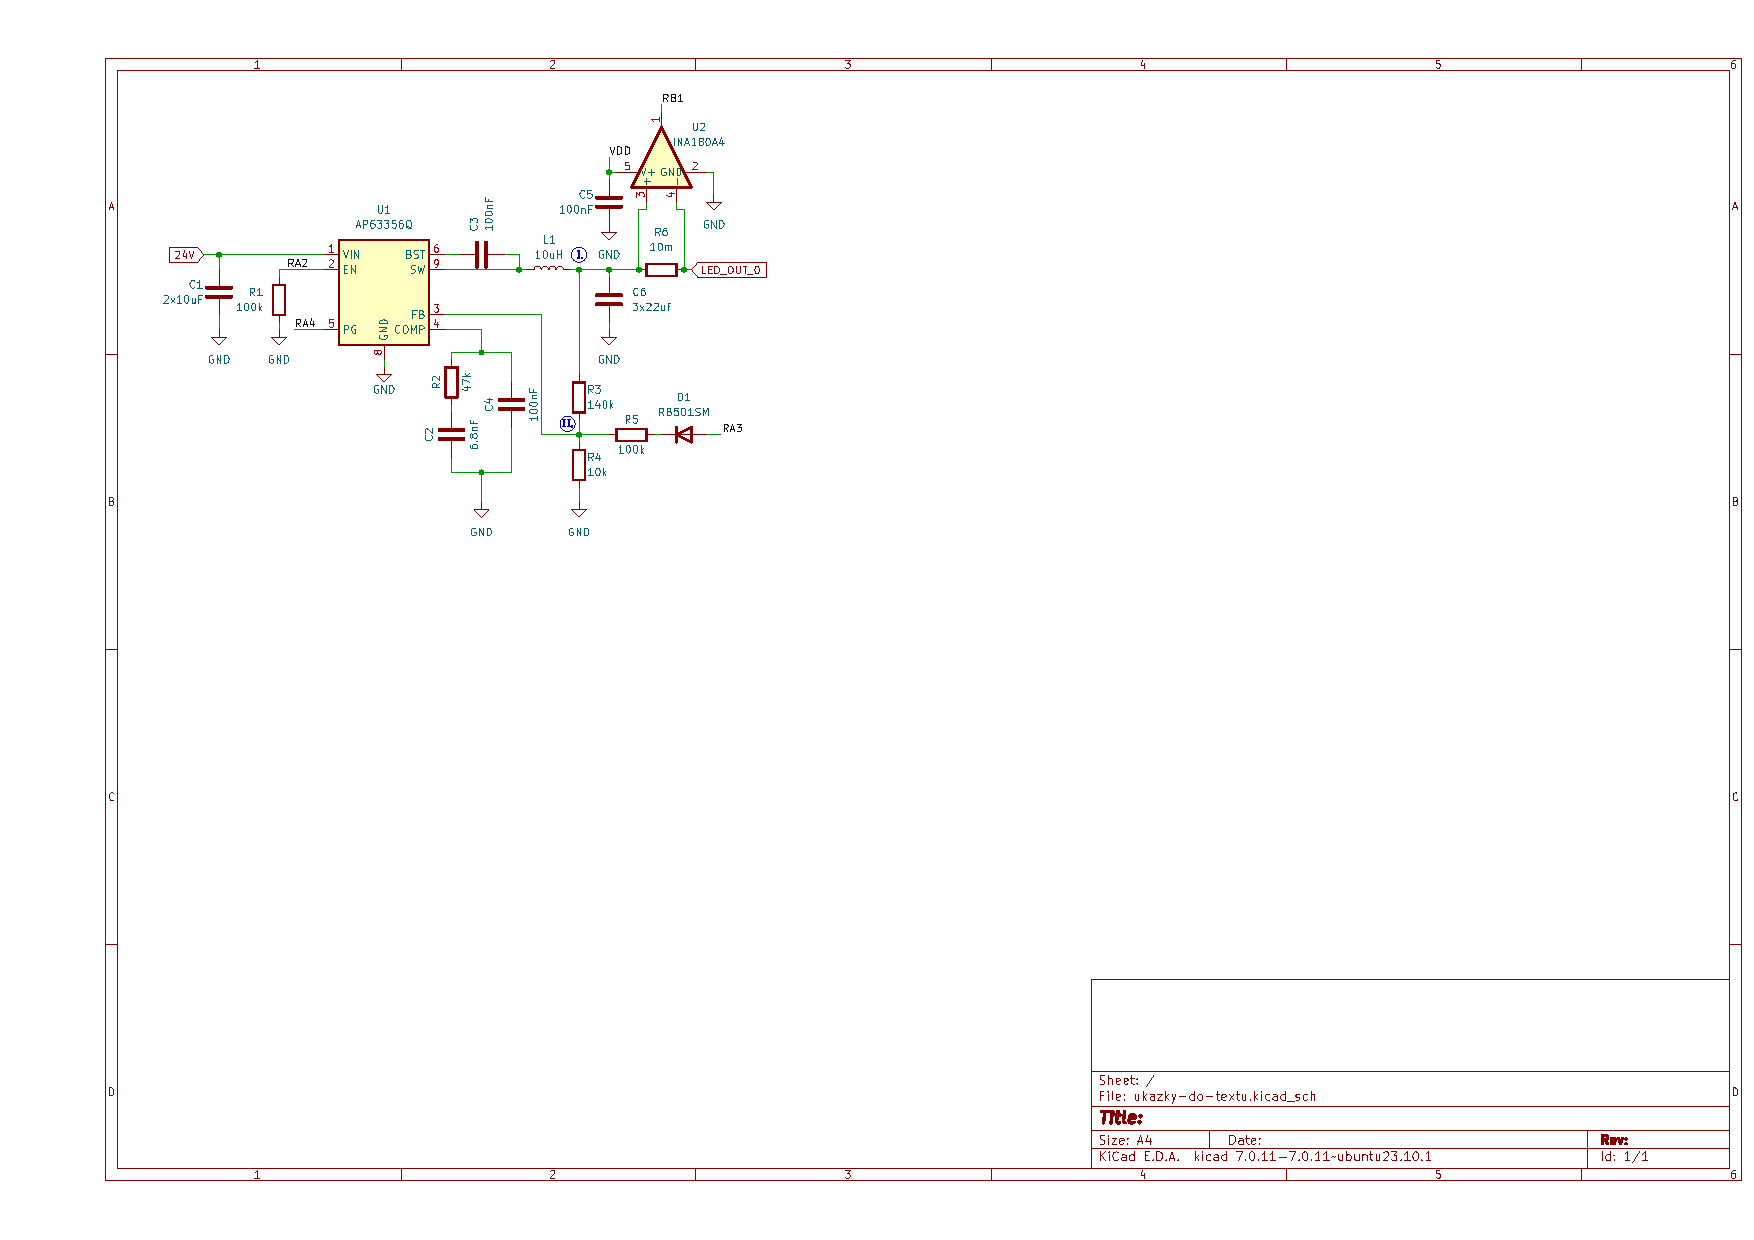
\includegraphics
        [
            width=\textwidth, 
            page=1, 
            trim=2.5cm 11.5cm 16cm 1.5cm, 
            clip
        ]{obrazky/exportovane/ukazky-do-textu.pdf}
        \caption{Zjednodušené schéma ovladače \acs{led}. Vytvořeno v~KiCad 7.0.}
        \label{fig:led-board-simp-schema}
    \end{figure}

    
\subsubsection{Popis schématu a výpočty hodnot součástek}
    Zjednodušené schéma pro jeden ovládaný kanál se nachází na obr.~\ref{fig:led-board-simp-schema}, při výpočtech bude použito označení součástek z tohoto schématu. Úplné schéma modulu pak lze nalézt v příloze~\ref{priloha:schema-led-board}.

    Jako buck kontrolér je zvolen čip AP63356Q vyvinutý společností Diodes incorporated, jedná se o úspornou a velmi malou součástku, která v sobě integruje oba potřebné MOSFET tranzistory a spíná s pevně danou frekvencí \(f_{SW}=\qty{450}{kHz} \) ~\cite{Diodes_AP63356Q}. Pro snímání proudu poslouží čip INA180A4 firmy Texas Instruments~\cite{TI_INA180A4}.

    Z obrázku je vidět, že pro ovládání jednoho kanálu \acs{led} pásků jsou využity 4 piny \acs{mcu}. RA4 a RB1 fungují jako vstupy, RA2 a RA3 pak jako výstupy. Rezistor \(R_{1}\) drží buck měnič ve vypnutém stavu, dokud mikrokontrolér nenastaví hodnotu pinu RA2 na logickou 1. Pin RA4 je pak čipem (U1) stažen k zemi vždy, když na výstupu není odpovídající nastavené napětí.  
    
    Nastavení výstupního napětí měniče je dosaženo za pomoci zpětnovazební smyčky mezi výstupním uzlem (I.) a zpětnovazebním pinem FB (uzel II.). V uzlu II. je drženo konstantní napětí \qty{0.8}{V}~\cite{Diodes_AP63356Q}, poměrem rezistorů R3 a R4 je pak definováno výstupní napětí. Zvolíme hodnotu odporu \(R_{4} = \qty{10}{k\ohm}\), pro maximální požadované napětí \(U_{outMAX} = \qty{12}{V}\) platí:
    \begin{equation}
        R_{3} = R_{4}\cdot \left(\frac{U_{outMAX} }{\num{0.8}}-1\right) = \qty{10}{k}\cdot \left(\frac{12}{\num{0.8}}-1\right) = \qty{140}{k\ohm}
    \end{equation} 
    Na pin RA3 mikrokontroléru je přivedeno analogové napětí z periferie \acs{dac} popř. \acs{pwm} signál. Skrze rezistor R5 (a ochrannou diodu) pak teče proud do rezistoru R4, úbytek napětí na tomto rezistoru je ale konstantní (\qty{0.8}{V}) a tedy je konstantní i proud rezistorem. Z prvního Kirchhoffova zákona pak víme, že proud rezistorem R3 klesne o hodnotu proudu dodanou z pinu RA3, tím klesne také napětí na výstupu měniče a dojde ke ztlumení jasu \acs{led} pásku. Citlivost (nebo také rozsah) změny je definována hodnotou R5, snížením jeho hodnoty lze dosáhnout na výstupu ještě nižšího napětí. Pro hodnotu \(R_{5} = \qty{100}{k\ohm}\) zobrazenou ve schématu lze nejnižší možné napětí vypočítat následovně:
    \begin{equation}
        U_{outMIN} = \num{0.8}+R_{3} \cdot I_{3} = \num{0.8}+R_{3} \cdot \left(\frac{\num{0.8}}{R_{4}} - \frac{U_{VDD} - U_{D1}}{R_{4}+R_{5}} \right) 
    \end{equation}  
    Kdy \(U_{VDD} = \qty{3.3}{V}\) je maximální napětí pinu RA3 a \(U_{D1}=\qty{0.35}{V} \) je prahové napětí zvolené diody. Po dosazení získáme:
    \begin{equation}
        U_{outMIN} = \num{0.8}+\qty{140}{k} \cdot \left(\frac{\num{0.8}}{\qty{10}{k}} - \frac{\num{3.3} - \num{0.35}}{\qty{10}{k}+\qty{100}{k}} \right) = \qty{8.25}{V}
    \end{equation}  
    Toto napětí by mělo být dostatečně nízké k úplnému zhasnutí \acs{led} pásku.

    TODO: Kompenzace

    V dalším kroku je stanovena hodnota induktoru L1. Výrobce doporučuje zvolit zvlnění proudu induktorem (ripple) \(\Delta I_{L}  \) jako 30 až \qty{50}{\percent} maximálního odběru. Pro výpočet induktoru je uvažován maximální povolený proud čipem, tím je zajištěno, že čip bude fungovat i po překročení maximálního očekávaného proudu \(I_{max} = \qty{1.66}{A} \). Při zvolení střední hodnoty \qty{40}{\percent} získáme:
    \begin{equation}
        \Delta I_{L} = \num{0.4}\cdot I_{IC-max} = \num{0.4} \cdot  \num{3.5} = \qty{1.4}{A}
    \end{equation}
    Odpovídající hodnota indukčnosti je vypočtena následujícím vztahem:
    \begin{equation}
        L_{1} = \frac{U_{outMAX}\cdot (U_{in} -U_{outMAX} ) }{U_{in} \cdot \Delta I_{L}\cdot f_{SW}  }
    \end{equation}
    Po dosazení získáme:
    \begin{equation}
        L_{1} = \frac{12\cdot (24 -12 ) }{24 \cdot \num{1.4}\cdot \qty{450}{k}  } = \qty{9.52}{\micro H}
    \end{equation}
    Zvolíme nejbližší běžně používanou hodnotu \(L_{1} = \qty{10}{\micro H}\). 

    Pro vstupní (C1) a výstupní (C6) kapacitu použijeme hodnoty doporučené výrobcem, stejně tak pro bootstrap kondenzátor C3. 
    
    Poslední součástkou zůstává měřicí rezistor R6. Tímto rezistorem protéká celý výstupní proud měniče, v rámci minimalizace ztrátového výkonu by měl mít tedy co nejmenší odpor. Musíme ovšem také brát v potaz rozsah měřicího zesilovače INA180A4. Tato součástka se vyrábí v několika variantách, byla zvolena varianta s nejvyšším ziskem \(G_{INA}=200 \) pro zachování co nejnižší hodnoty rezistoru, výstupní napětí zesilovače je v rozsahu 0 až \qty{3.3}{V} (VDD mikrokontroléru).
    Při maximálním očekávaném proudu chceme dosáhnout horní hranice rozsahu zesilovače, z této podmínky vyplývá vztah pro výpočet odporu rezirtoru R6:
    \begin{equation}
        R_{6} = \frac{U_{VDD}}{I_{max} \cdot G_{INA} } = \frac{\num{3.3}}{\num{1.66}\cdot 200} = \qty{9.94}{m\ohm}
    \end{equation} 
    Zvolíme blízkou hodnotu \(R_{6} \) = \qty{10}{m\ohm}.


\subsubsection{Očekávané parametry}
    Pro výpočet výstupního zvlnění (v uzlu I.) chybí údaj o ekvivalentním sériovém odporu (ESR) výstupních kondenzátorů (C6), který výrobce neuvádí. Vyjdeme tedy z typické hodnoty pro keramický kondenzátor \(ESR=\qty{15}{m\ohm}\)~\cite{wikipedia2024esr}, kdy počítáme s paralelní kombinací tří kondenzátorů.
    Očekávané výstupní zvlnění je tedy přibližně:
    \begin{equation}
        \Delta U_{out} = \Delta I_{L} \cdot  \left(\frac{ESR}{3}+\frac{1}{8\cdot f_{SW} \cdot C_{6} }\right) 
    \end{equation} 
    \begin{equation}
        \Delta U_{out} = \num{1.4} \cdot  \left(\frac{\qty{15}{m}}{3}+\frac{1}{8\cdot \qty{450}{k} \cdot 3\cdot \qty{22}{\micro\,} }\right)  = \qty{13}{mV}
    \end{equation} 

    \textit{TODO: Zde velký question: Pokusit se o přesnější výpočet ztrát a účinnosti nebo se odkázat na kalkulačku výrobce, která stejně bude nejpřesnější?}
    % Jestli chceš tak nebo tak je to celkem jedno. Nicméně kalkulačka výrobce vůbec nemusí být nejpřesnější. Naopak výrobci kolikrát kecají a ukáží ti lepší výsledek.

\subsection{Tvorba \acs{dps}}
    Jak již bylo zmíněno v úvodu kapitoly, jedná se o dceřinnou desku pro obecný modul periferie, čímž jsou jasně určeny její maximální rozměry. Stejně jako u předešlých návrhů, i zde je použita čtyřvrstvá struktura viz obr.~\ref{fig:ridici-jednotka-stackup-dps}. Vizualizace návrhu se nachází na obr.~\ref{fig:perif-led-dps} spolu s ukázkou sesazení s obecným modulem periferie. 


    \begin{figure}[!ht]
        \centering
        \begin{tikzpicture}
            % Include the image
            \node[anchor=south west,inner sep=0] (image) at (0,0) {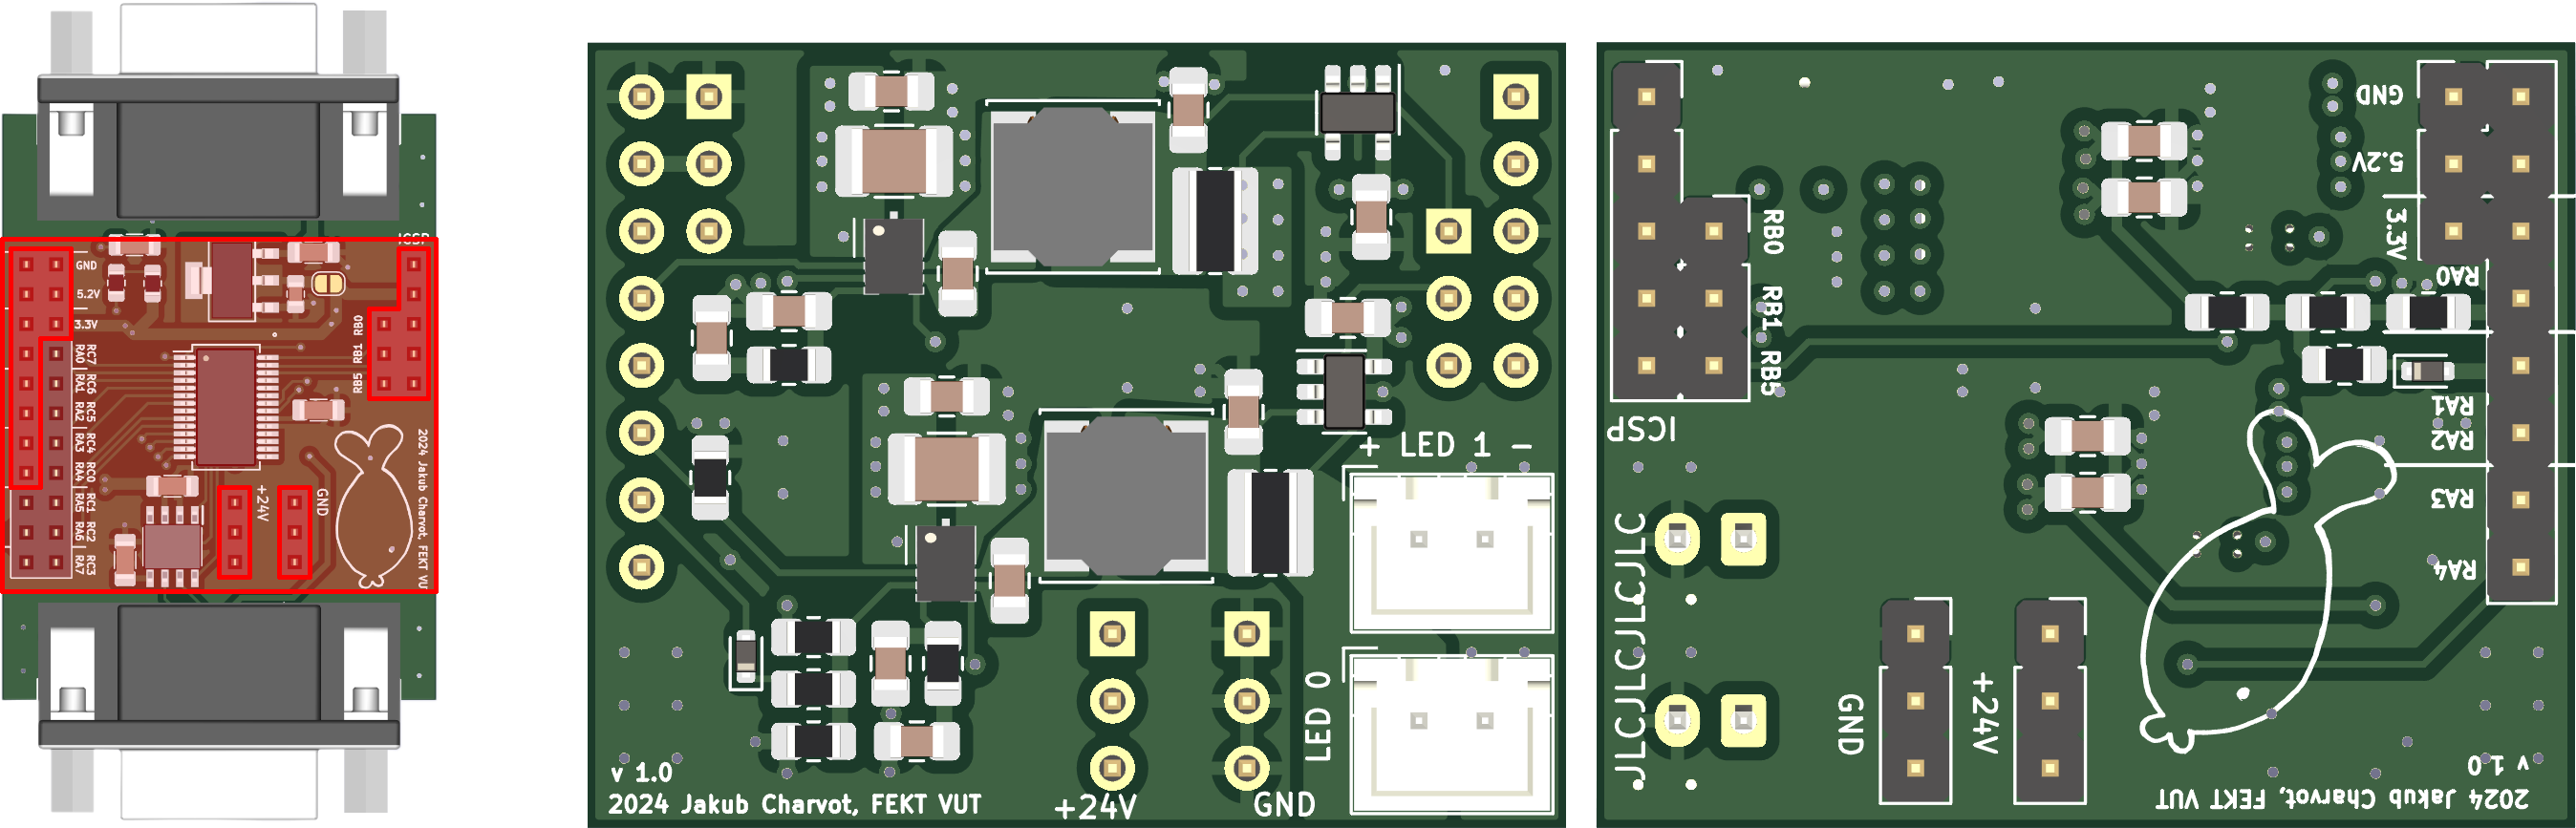
\includegraphics[width=0.8\textwidth]{obrazky/dps/ledboard-combined.png}};
            
            \draw[dashed] (10.1,0.02) -- (12.5,0.02);
            \draw[<->,thick] (12.5,0.02) -- (12.5,3.66);
            \draw[dashed] (12.5,3.66) -- (10.1,3.66);
            \node[anchor=west] at (12.5,1.83)  {\qty{36}{mm}};

            \draw[dashed] (2.75,0.02) -- (2.75,-0.5);
            \draw[<->,thick] (2.75,-0.6) -- (7.3,-0.6);
            \draw[dashed] (7.3,-0.6) -- (7.3,0.02);
            \node[anchor=south] at (5,-0.6)  {\qty{57}{mm}};

            \draw[dashed,thick,color=red] (2.75,0.02) -- (2.05,1.1);
            \draw[dashed,thick,color=red] (2.75,3.66) -- (2.05,2.7);
        \end{tikzpicture}
        \caption{Vizualizace \acs{dps} periferie \acs{led} osvětlení.}
        \label{fig:perif-led-dps}
    \end{figure}

    Za účelem zvětšení plochy pro umístění součástek byly z konektorů obecného modulu vyvedeny pouze některé piny, i přesto bylo nakonec potřeba umístit komponenty také na spodní stranu \acs{dps}. Rozmístění součástek je obdobné pro oba měniče napětí a respektuje doporučení výrobce a tedy i obecná pravidla pro návrh měničů napětí~\cite{Diodes_AP63356Q}. Je kladen důraz na to, aby smyčka ze spínacího uzlu přes výstupní kapacitu a zem zpět do kontroléru byla co nejkratší a vedena za pomoci polygonů. Stejně tak vstupní kapacitor je umístěn přímo vedle vstupních pinů kontroléru.
    




\section{Senzor \acs{ph}}
\label{sec:perif-sensor-ph}

\section{Ovládání 230V periferií}
\label{sec:perif-230v}
Jak vyplývá z~požadavků zařízení a přehledu používané akvaristické techniky, pro automatizovaný provoz akvária je nutné umožnit řídicí jednotce ovládat několik okruhů se síťovým napětím a spínat tak zvlášť zakoupené hotové spotřebiče pracující s~tímto napětím. Jedná se typicky o~ohřev vody, filtraci, popř. některé druhy osvětlení. 

\begin{figure}[h!]
    \centering
    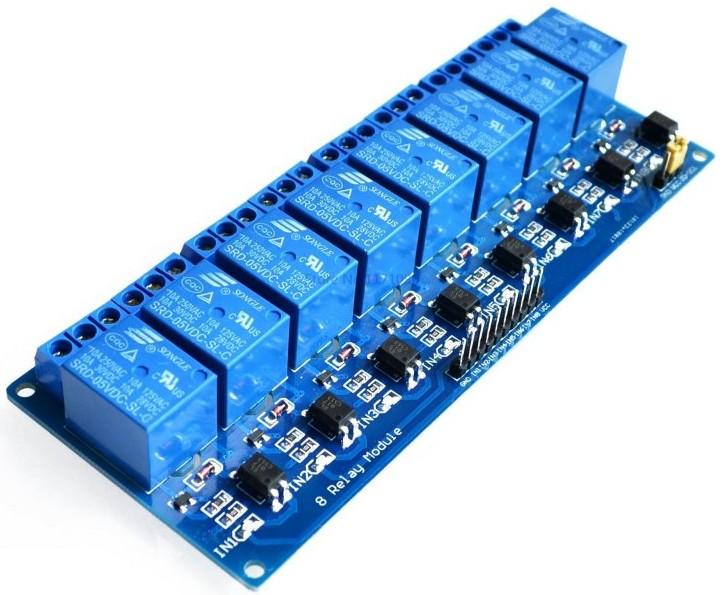
\includegraphics[width=0.6\textwidth]{obrazky/230/rele.jpg}
    \caption{TODO vyměnit: Relé modul, ilustrační foto. Převzato z~\cite{eshop-laskakit-rele}.}
    \label{fig:obrazky-230-rele-jpg}
\end{figure}


Aby uživatel mohl spínaná zařízení bezpěčně připojit bez nutnosti odborné způsobilosti, nachází se na hlavním šasi zařízení čtyři standartní zásuvky (typ E) s~jednofázovým napětím \qty{230}{V}. Fázové vodiče jsou uvnitř zařízení přerušeny spínacími relé. Je použit předpřipravený modul disponující osmi relé~\cite{eshop-laskakit-rele}, čtyři z nich tedy zůstanou nevyužité a slouží jako rezerva pro případ poškození některého z~používaných relé nebo při potřebě budoucího rozšíření o~další zásuvky. 

Z~důvodu nedostatku pinů na mikrokontroléru řídicí jednotky (ESP32) je k~relé modulu připojen ještě jeden externí modul a to expandér \acs{gpio} pinů komunikující přes sběrnici \acs{i2c}~\cite{eshop-laskakit-expander}. Z~pohledu mikrokontroléru jsou tak všechny zásuvky ovládány pomocí dvou \acs{gpio} pinů (\acs{sda}, \acs{scl}), které je navíc možné dále využít pro připojení jiných periferií jako např. O\acs{led} displaje pro zobrazení stavu zařízení.

Relé na použitém modulu potřebuje pro spolehlivé sepnutí napětí alespoň \qty{5}{V}, logické signály řídicí jednotky ale pracují s napětím pouze \qty{3.3}{V}. Ze schématu na obr.~\ref{fig:relay-board-simp-schema} je vidět, že použitý relé modul je spínán signálem logické nuly, tímto způsobem je problém s rozdílnou úrovní napájení elegantně vyřešen. 

\begin{figure}[h!]
    \centering
    % trim=left bottom right top
    \includegraphics
    [
        width=\textwidth, 
        page=3, 
        trim=2.5cm 14.5cm 18cm 1.5cm, 
        clip
    ]{obrazky/exportovane/ukazky-do-textu.pdf}
    \caption{Schéma jednoho kanálu relé modulu. Vytvořeno v~KiCad 7.0.}
    \label{fig:relay-board-simp-schema}
\end{figure}

Do budoucna by bylo možným zlepšením a rozšířením této práce zahrnutí obou zmíněných modulů přímo na \acs{dps} řídicí jednotky. 




\chapter{Software}
    Tato kapitola se věnuje popisu návrhu softwaru pro jednotlivé části systému řízení akvária. Jak již bylo zmíněno v předchozích kapitolách, systém se skládá z řídicí jednotky, ke které jsou připojeny jednotlivé periferie a která komunikuje s webovým serverem za pomoci WiFi. Každá ze zmíněných částí pak potřebuje vlastní zdrojový kód. 
    
    K programování a testování byla použita dvě vývojová prostředí. Visual Studio Code je open source řešení spravované společností Microsoft a díky široké škále doplňků umožňuje velmi univerzální použití. S přidaným rozšířením ESP-IDF je také preferovaným prostředím společnosti Espressif, bylo tedy využito pro tvorbu kódu řidicí jednotky, stejně tak i pro webové rozhraní. Pro programování periferií bylo zvoleno prostředí MPLAB X. Jedná se o řešení společnosti Microchip určené speciálně pro programování mikrokontrolérů této firmy. Součástí je kromě samotného editoru také kompilátor, možnost debugování kódu nebo modul zvaný Code Configurator sloužící pro generování jednoduchého HAL (Hardware Abstraction Level) kódu.

    V této chvíli software odpovídá podobě zbytku zařízení -- tedy jedná se o prototyp určený primárně k demonstraci funkce zařízení. Aby byl kód použitelný v reálné aplikaci a choval se zde spolehlivě, je potřeba podrobit jej rozsáhlejšímu testování a také lépe ošetřit chování zařízení v různých nežádoucích stavech.   

% \clearpage
\section{Architektura}
    Na obr.~\ref{fig:sw-blokove-schema} se nachází blokové schéma systému z pohledu softwaru. Obrázek slouží primárně pro lepší orientaci čtenáře v této kapitole, obsahuje pouze klíčové části a některé věci zjednodušuje. Podrobněji se jednotlivým blokům věnují další podkapitoly. Obdélník popsaný v obrázku jako \uv{Periferie} popisuje strukturu kódu platnou pro všechny periferie, je ale samozřejmé, že periferií této struktury bude v systému připojeno vícero.

    Propojení přerušovanými šipkami v obrázku značí komunikaci mezi dvěma částmi s odlišným programem. Z hlediska internetové komunikace se navržené zařízení chová jako klient, tedy neposlouchá na žádném portu a z vnější sítě není nijak dostupné. Webový server disponuje datovým rozhraním (API), kterého se zařízení v pravidelných intervalech dotazuje na případné změny konfigurace a prostřednictvím kterého zasílá na server data ze svého běhu. Při komunikaci mezi řídicí jednotkou a periferiemi pak řídicí jednotka funguje jako \uv{master} a periferie odpovídají pouze v reakci na dotaz z její strany.

    % Blokove schema
    \begin{figure}[h!]
        \centering
        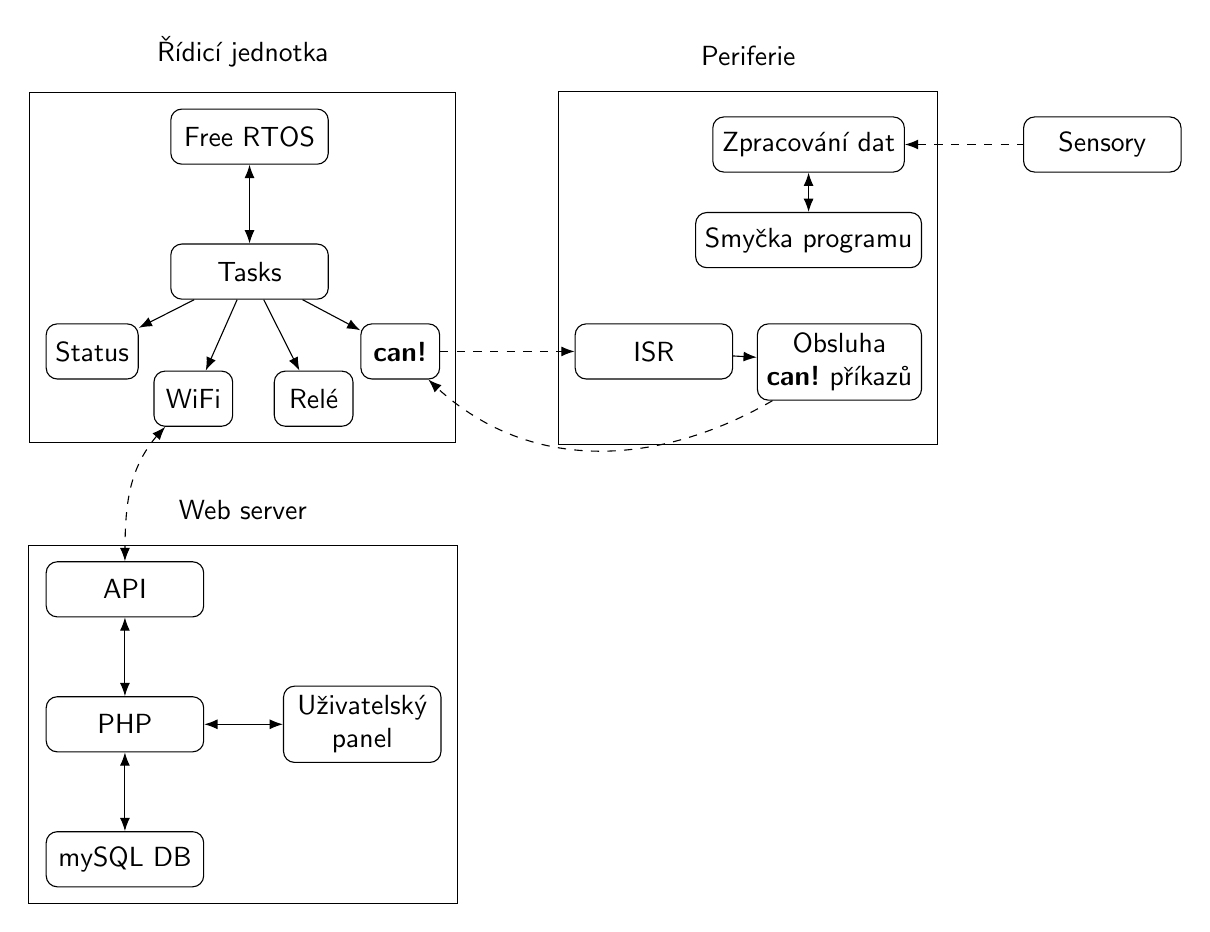
\begin{tikzpicture}[
            module/.style={%
        draw, rounded corners,
        minimum width=#1,
        minimum height=7mm,
        font=\sffamily,
        align=center
        },
    module/.default=2cm,
    >=LaTeX]
        
            % ridici
            \node[module] (freertos) {Free RTOS};
            \node[module, below=of freertos] (tasks) {Tasks};
            \node[module=1cm, below right=9mm and -7mm of tasks] (task1) {Relé};
            \node[module=1cm, below left= 9mm and -8mm of tasks] (task2) {WiFi};
            \node[module=1cm, below right= 3mm and 4mm of tasks] (task3) {\acs{can}};
            \node[module=1cm, below left= 3mm and 4mm of tasks] (task4) {Status};

            \node[fit=(task1) (task2) (task3) (task4) (freertos), draw, inner sep=2mm,label={[yshift=2mm, font=\sffamily]Řídicí jednotka}] (fitridici) {};
            % Connections
            \foreach \i in {1,2,3,4}
                \draw[->] (tasks)--(task\i);
            \draw[<->] (tasks)--(freertos);

            % WS
            \node[module, below=1.5cm of {task4.west|-fitridici.south}, anchor=north west] (api) {API};
            \node[module, below=of api] (php) {PHP};
            \node[module, below=of php] (mysql) {mySQL DB};
            \node[module, right= of php] (userweb) {Uživatelský \\panel};
            \node[fit={(php) (userweb) (api) (mysql) (mysql-|fitridici.west) (mysql-|fitridici.east) }, draw, inner xsep=\pgflinewidth, inner ysep=2mm, label={[yshift=2mm, font=\sffamily]Web server}] (fitWS) {};
            \draw[<->] (api)--(php);
            \draw[<->] (php)--(mysql);
            \draw[<->] (php)--(userweb);
        
            % perif
            \node[module, right=1.5cm of {task3-|fitridici.east}] (isr) {ISR};
            \node[module, right=3mm of isr.north east, anchor=north west] (can) {Obsluha\\\acs{can} příkazů};
            \node[module, above= 7mm of can.north east, anchor=south east] 
                (programloop) {Smyčka programu};
            \node[module, above=5mm of programloop] (dataprocess) {Zpracování dat};
            
            \node[fit={(can) (isr) (dataprocess|-fitridici.south) (dataprocess|-fitridici.north)}, draw, inner xsep=2mm, inner ysep=\pgflinewidth, label={[yshift=2mm, font=\sffamily]Periferie}] (fitperif) {};
            \node[module, right=1.5cm of dataprocess] (sensory) {Sensory};
            \draw[->] (isr)--(can);
            \draw[<->] (programloop)--(dataprocess);
            
            %arrow between boxes
            \draw[<->,dashed] (task2) to [out=-135,in=90] (api);
            \draw[->,dashed] (task3)--(isr);
            \draw[->,dashed] (can) to [out=-150,in=-45] (task3);
            \draw[<-,dashed] (dataprocess) -- (sensory);
        \end{tikzpicture}
        
        \caption{Zjednodušená architektura softwaru systému.}
        \label{fig:sw-blokove-schema}
    \end{figure}

    Jelikož jsou řídicí jednotka i periferie programovány ve stejném jazyce (C/C++), lze mezi nimi část kódu sdílet. Tímto způsobem lze částečně předejít chybám v komunikaci modulů mezi sebou. Společná část kódu obsahuje definice datových typů a konstant používaných při komunikaci po sběrnici \acs{can}.  

\section{Popis \acs{can} komunikace}
    Protokol \acs{can} je poměrně rozsáhlý a velká část organizace komunikace je řešena přímo hardwarovou periferií mikrokontroléru. Pro úspěšnou a efektivní komunikaci je potřeba nastavit oba typy mikrokontrolérů stejně a stanovit společný standart komunikace. Systém popsaný v této práci pracuje s frekvencí \qty{125}{kHz} a používá standartní strukturu rámců s identifikátorem zprávy dlouhým 11 bitů (standart \acs{can} 2.0B umožňuje také délku 29 bitů). Struktura datového rámce je zobrazena na obr.~\ref{fig:obrazky/can-frame.png }. Sběrnice \acs{can} má implementovaný princip arbitrace, pokud začne komunikovat více zařízení současně, odešle se zpráva mající identifikátor s nejvyšší prioritou. Logická nula se jeví na sběrnici jako dominantní, jednička naopak jako recesivní. Pokud zařízení odesílá recesivní signál a zároveň čte ze sběrnice signál dominantní, znamená to pro něj ztrátu arbitace a přestává vysílat, jelikož na sběrnici je v danou chvíli vysílaná zpráva s vyšší prioritou. Po skončení vysílání pak přerušené zařízení pokus opakuje.
    
        \begin{figure}[h!]
            \centering
            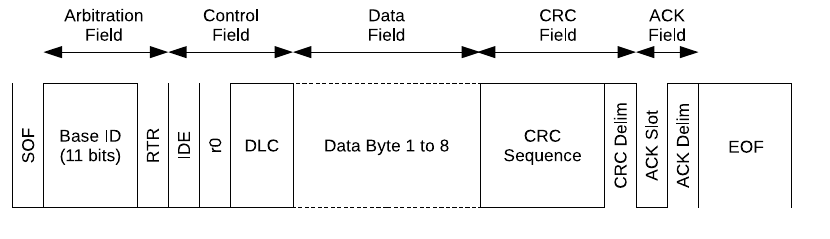
\includegraphics[width=0.8\textwidth]{obrazky/can-frame.png}
            \caption{Struktura datového rámce sběrnice \acs{can}. Převzato z~\cite{esp32-datasheet}}
            \label{fig:obrazky/can-frame.png   }
        \end{figure}
        

    V navrženém systému nese identifikátor zprávy dvě informace. První tři odesílané bity značí typ zprávy. Rozlišena je zpráva určené všem jednotkám (BR -- Broadcast), zpráva od řídicí jednotky k periferiím (TS -- master To Slave), od periferie zpět k řídicí jednotce (TM -- slave To Master) a debug zpráva sloužící k odeslání diagnostických dat nezávisle na ostatní komunikaci. Zbylých 8 bitů pak tvoří adresu jednotky odesílající zprávu (v případě TM) resp. zprávu přijímající (v případě TS). 
    
    \subsection{Adresace}
    Adresy jednotlivých modulů by měly být po startu systému nebo připojení nové jednotky automaticky přiděleny tak, aby nedošlo ke kolizi adres ani v případě připojení několika sensorů stejného typu. Princip adresace spočívá v sérii několika BR zpráv. Po startu systému pošle řídicí jednotka požadavek na adresaci, jako odpověď odešlou jednotky periferíí své unikátní sériové číslo přičemž pouze jedna ze zpráv vyhraje arbitraci. Řídicí jednotka odpoví zprávou, která obsahuje sériové číslo úspěšné jednotky a přidělenou osmibitovou adresu. Následně zopakuje požadavek adresace a odpoví již pouze jednotky bez adresy, po dokončené adresaci pak neodpoví žádná jednotka. Pokud je do běžícího systému připojena nová periferie, odešle sama BR zprávu s požadavkem na přidělení adresy.

    Ačkoliv je tento princip vymyšlen, v rámci prototypu prozatím není implementován a otestován a každý typ periferie má pevně přidělenou adresu, lze tedy připojit pouze jednu periferii stejného typu. V současné chvíli je toto řešení dostačující.



\section{Firmware řídicí jednotky}
    Firma Espressif nabízí pro své mikrokontroléry dva základní frameworky. Oba jsou vyvíjeny jako open-source a jsou tedy také volně dostupné pro jakékoliv použití. Univerzálním řešením vhodným i pro komerční aplikace je ESP-IDF (Espressif Integrated Development Framework). Pro hobby projekty lze využít také Arduino framework, který je taktéž oficiálně podporovaný. Poslední novinkou je pak možnost programování v jazyce Rust namísto klasického C/C++, tento projekt je vytvářen komunitou uživatelů za podpory společnosti Espressif, prozatím ale nebyla oficiálně vydána stabilní verze. 

    V rámci této práce je využit framework ESP-IDF spolu s několika volně dostupnými knihovnami. Toto řešení již obsahuje HAL kód pro práci s periferiemi MCU, není tedy potřeba pracovat přímo s procesorovými registry. Framework má také podporu pro jednoduchý operační systém FreeRTOS, který je rovněž v této práci využit~\cite{espressif-idf}. 

    \subsection{FreeRTOS}
        Systém FreeRTOS umožňuje vytvářet tzv. tasky neboli samostatné procesy které běží z pohledu uživatele paralelně. Jelikož má zvolený mikroprocesor dvě jádra, mohou dva tasky běžet skutečně paralelně, více procesů se pak ve svém běhu střídá a běží tak přerušovaně, dá se říci pseudoparalelně. O tuto režii se stará samotný operační systém a vývojář má několik možností, jak tento proces ovlivnit. V případě vytížení procesoru systém přiděluje čas na základě nastavených priorit a dá přednost tasku s vyšší prioritou, může se tak stát, že některý proces zůstane pozastaven na dlouhou dobu. Při tvorbě kódu je potřeba mít toto na paměti, vhodně zvolit priority tasků a také průběžně sledovat vytížení procesoru jednotlivými tasky.  

        Aby byl kód tzv. thread-safe, tedy bezpečný pro přístup z více vláken, je potřeba ošetřit případy, kdy více tasků pracuje se stejnými daty nebo přistupuje ke stejné periferii mikrokontroléru. K tomuto účelu FreeRTOS nabízí synchronizační objekty jako jsou mutexy, semafory případně fronty. 

    \subsection{Indikace stavu zařízení}
    \label{kap:indikace-stavu-ridici-jednoty}
        Šasi řídicí jednotky je vybaveno adresovatelným barevným \acs{led} páskem sestávajím ze čtyř diod jejichž úkolem je signalizovat uživateli stav zařízení. Jednotlivé stavy spolu s popisem diod jsou zobrazeny na obr.~\ref{fig:stavove-led-mainboard}. Každý task, který je součástí procesu diagnostiky má svou vlastní globální proměnnou do které ukládá svůj stav. Dvakrát za vteřinu se pak spustí jednoduchá diagnostická funkce (běží v rámci vlastního tasku), která jednotlivé stavové proměnné přečte, vyhodnotí celkový stav zařízení a aktualizuje barvu stavových \acs{led}. 
        \begin{figure}[h!]
            \centering
            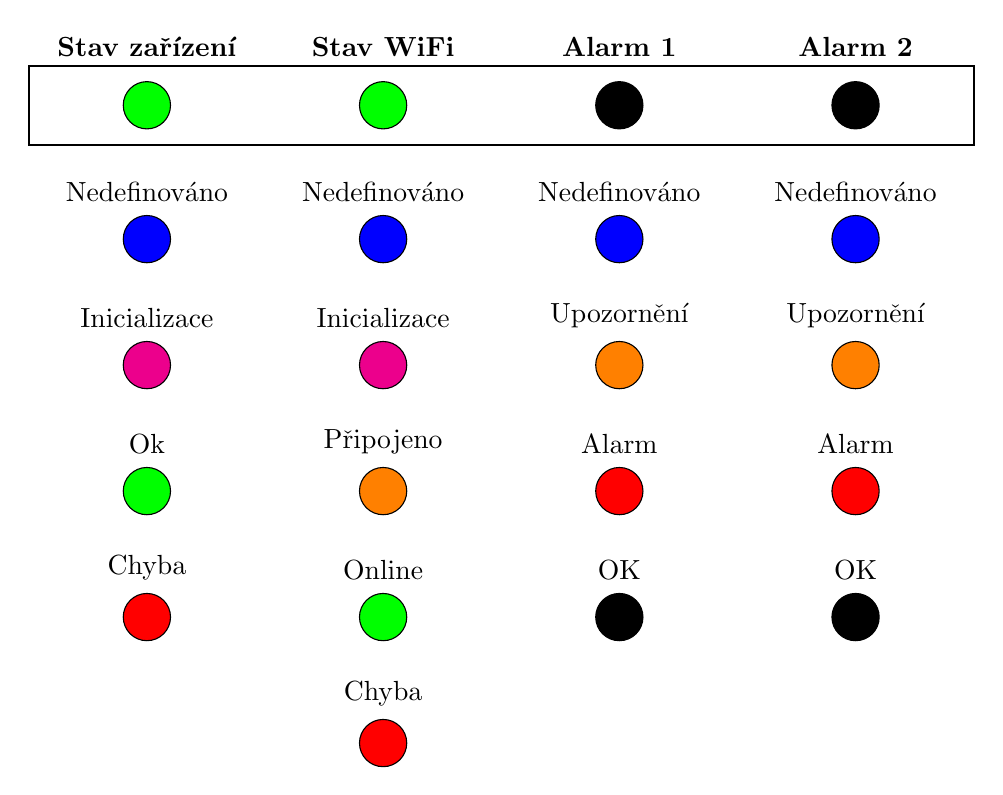
\begin{tikzpicture}
                % Draw a rectangle
                \draw[thick] (0,0) rectangle (3*4,1);
                
                % Draw and fill four colorful circles
                \filldraw[fill=green,draw=black,thin]  (3*0.5, 0.5) circle (0.3) node[align=center,above=0.5] {\textbf{Stav zařízení}};
                \filldraw[fill=green,draw=black,thin]  (3*1.5, 0.5) circle (0.3) node[align=center,above=0.5] {\textbf{Stav WiFi}};
                \filldraw[fill=black,draw=black,thin]  (3*2.5, 0.5) circle (0.3) node[align=center,above=0.5] {\textbf{Alarm 1}};
                \filldraw[fill=black,draw=black,thin]  (3*3.5, 0.5) circle (0.3) node[align=center,above=0.5] {\textbf{Alarm 2}};

                % Draw and fill four colorful circles
                \filldraw[fill=blue,draw=black,thin]    (3*0.5, -1.5*0.8) circle (0.3) node[align=center,above=0.35] {Nedefinováno};
                \filldraw[fill=blue,draw=black,thin]    (3*1.5, -1.5*0.8) circle (0.3) node[align=center,above=0.35] {Nedefinováno};
                \filldraw[fill=blue,draw=black,thin]    (3*2.5, -1.5*0.8) circle (0.3) node[align=center,above=0.35] {Nedefinováno};
                \filldraw[fill=blue,draw=black,thin]  (3*3.5, -1.5*0.8) circle (0.3) node[align=center,above=0.35] {Nedefinováno};

                % Draw and fill four colorful circles
                \filldraw[fill=magenta,draw=black,thin] (3*0.5, -3.5*0.8) circle (0.3) node[align=center,above=0.35] {Inicializace};
                \filldraw[fill=magenta,draw=black,thin] (3*1.5, -3.5*0.8) circle (0.3) node[align=center,above=0.35] {Inicializace};
                \filldraw[fill=orange,draw=black,thin]  (3*2.5, -3.5*0.8) circle (0.3) node[align=center,above=0.35] {Upozornění};
                \filldraw[fill=orange,draw=black,thin]  (3*3.5, -3.5*0.8) circle (0.3) node[align=center,above=0.35] {Upozornění};

                % Draw and fill four colorful circles
                \filldraw[fill=green,draw=black,thin]   (3*0.5, -5.5*0.8) circle (0.3) node[align=center,above=0.35] {Ok};
                \filldraw[fill=orange,draw=black,thin]  (3*1.5, -5.5*0.8) circle (0.3) node[align=center,above=0.35] {Připojeno};
                \filldraw[fill=red,draw=black,thin]   (3*2.5, -5.5*0.8) circle (0.3) node[align=center,above=0.35] {Alarm};
                \filldraw[fill=red,draw=black,thin]  (3*3.5, -5.5*0.8) circle (0.3) node[align=center,above=0.35] {Alarm};

                % Draw and fill four colorful circles
                \filldraw[fill=red,draw=black,thin]     (3*0.5, -7.5*0.8) circle (0.3) node[align=center,above=0.35] {Chyba};
                \filldraw[fill=green,draw=black,thin]   (3*1.5, -7.5*0.8) circle (0.3) node[align=center,above=0.35] {Online};
                \filldraw[fill=black,draw=black,thin]   (3*2.5, -7.5*0.8) circle (0.3) node[align=center,above=0.35] {OK};
                \filldraw[fill=black,draw=black,thin]   (3*3.5, -7.5*0.8) circle (0.3) node[align=center,above=0.35] {OK};

                % Draw and fill four colorful circles
                \filldraw[fill=red,draw=black,thin]     (3*1.5, -9.5*0.8) circle (0.3) node[align=center,above=0.35] {Chyba};
            \end{tikzpicture}
            
            \caption{Stavové \acs{led} řídicí jednotky.}
            \label{fig:stavove-led-mainboard}
        \end{figure}

    \subsection{Popis jednotlivých tasků}
        Řídicí jednotka vykonává současně několik funkcí. Komunikuje s periferiemi skrze sběrnci CAN, ovládá připojená relé a stavové diody. Kromě toho také komunikuje s webovým serverem prostřednictvím WiFi. Jednotlivé úlohy je třeba vykonávat periodicky, ovšem každou s jinou prioritou. Kód je proto rozdělen do několika tasků podle své funkce a priority. 

        K synchronizaci tasků jsou využity binární semafory. K převzetí semaforu ve {FreeRTOS} slouží funkce \texttt{xSemaphoreTake( xSemaphore, xBlockTime )}. Na řádku s touto funkcí kód čeká až do přijetí semaforu odeslaného jiným taskem nebo do vypršení času stanoveného druhým parametrem. 

        Každý z tasků začíná inicializací, kdy se jednorázově nastaví potřebné proměnné. Dále pokračuje nekonečnou smyčkou přerušenou vždy čekáním na semafor nebo neblokujícím zpožděním za pomocí funkce \texttt{vTaskDelay( const TickType\_t xTicksToDelay )}.

        % \begin{lstlisting}[language={[LaTeX]TeX}]
        %     \section{Balíček lstlistings}
        %     Pro vysázení zdrojových souborů je možné použít
        %         balíček \href{https://www.ctan.org/pkg/listings}%
        %         {\texttt{listings}}.
        %     Balíček zavádí nové prostředí \texttt{lstlisting} pro
        %         sazbu zdrojových kódů.
        %     \end{lstlisting}
        
        \subsubsection{Kontrolní proces -- \texttt{control\_task}}
            Jedná se o hlavní task programu co se týče samotného algoritmu. Na začátku běhu ve vhodném pořadí spustí ostatní tasky a provede vlastní inicializaci. Je spuštěna adresace zařízení na sběrnici CAN a od připojených periferií následně vyžádána informace o jejich typu, sériovém čísle a současnému stavu. Z perzistentní paměti flash je na základě sériového čísla načtena konfigurace jednotlivých modulů a samotného systému. 

            Ve smyčce je následně pravidelně prováděn sled několika operací. Pokud je to potřeba, dojde ke stažení nové konfigurace ze serveru, aktualizaci odpovídajích proměnných i paměti flash.  O nutnosti této operace rozhoduje \texttt{wifi\_task}.

            Dále jsou obslouženy periferie na sběrnici. Je vyžádán jejich status a dle typu také senzorická a provozní data. 

            Na základě konfigurace systému, získaných dat a reálného času je odeslán požadavek odpovídajícím akčím členům a aktualizován stav relé. Také je zpracován případný alarm, který je následně jiným taskem signalizován prostřednictvím stavových diod. 

            Dle nastavené periody jsou data získaná ze senzorů také odeslána na webový server.

        \subsubsection{Obsluha WiFi --  \texttt{wifi\_task}}
            V inicializační fázi tohoto tasku je vznešen požadavek na připojení k síti WiFi. V případě selhání nebo pozdějšího odpojení je pokus automaticky opakován. 
            
            V nekonečné smyčce pak task periodicky kontroluje dostupnost internetového připojení, dotazuje se serveru na poslední dostupnou verzi konfigurace a aktualizuje údaj o reálném čase (ten je následně uchován vnitřním \acs{rtc} časovačem mikrokontroléru).

        \subsubsection{Obsluha sběrnice CAN --  \texttt{can\_bus\_task}}
            Inicializuje potřebné GPIO piny a připraví potřebné proměnné. Ve smyčce pak pravidelně kontroluje příchozí zprávy na sběrnici (zejména typu Broadcast, které mohou být odeslány periferiemi bez vyzvání). Příchozí zprávy filtruje a pomocí front předává dalším taskům. Na začátku vždy čeká na kontrolní semafor značící požadavek na vyčtení sběrnice. Pokud není vyslán požadavek, čekání na semafor vyprší a sběrnice je zkontrolována s danou periodou.

            \subsubsection{Obsluha WiFi --  \texttt{wifi\_task}}
            V inicializační fázi tohoto tasku je vznešen požadavek na připojení k síti WiFi. V případě selhání nebo pozdějšího odpojení je pokus automaticky opakován. 
            
            V nekonečné smyčce pak task periodicky kontroluje dostupnost internetového připojení, dotazuje se serveru na poslední dostupnou verzi konfigurace a aktualizuje údaj o reálném čase (ten je následně uchován vnitřním \acs{rtc} časovačem mikrokontroléru).

        \subsubsection{Indikace stavu --  \texttt{status\_update\_task}}
            Zpracovává stavové proměnné ostatních tasků a na základě těchto dat vyhodnocuje stav zařízení. Tento stav následně indikuje za pomoci stavových diod, jak bylo popsáno v kapitole~\ref{kap:indikace-stavu-ridici-jednoty}.



\section{Firmware periferií}
    Jak bylo popsáno v kapitole~\ref{sec:modul-periferie}, všechny periferie mají stejné jádro. Ve všech pracuje stejný mikrokontrolér (PIC18F26), stejným způsobem pracují se sběrnicí CAN a také část příkazů na sběrnici je všem periferiím společná. Rozdíl mezi periferiemi je daný pouze připojenými sensory. Ty vyžadují vždy specifické nastavení vstupních a výstupních pinů, zpracování dat a jejich odeslání skrze sběrnici CAN. 

    Tato struktura je replikována také ve zdrojovém kódu. Pro všechny periferie existuje společný projekt, kdy základní kód zůstává vždy stejný. Pro sestavení a nahrání programu do konkrétního modulu je potřeba upravit hlavičkový soubor \texttt{device\_type.h}. Tento soubor nastaví typ zařízení a následně za pomoci preprocesorových direktiv vloží do projektu pouze odpovídající knihovny. Výňatek z tohoto souboru je zde uveden jako výpis~\ref{lst:devicetype}. Stejným principem je kód větven na všech místech, kde je toto potřeba. 

    Program sestává ze dvou hlavních částí. Nejprve je to fáze incializace, kdy dojde k nastavení potřebných registrů a proměnných. Poté zařízení vstupuje do nekonečné smyčky. V té jsou periodicky vyčítána data z připojených senzorů resp. ovládány akční členy.  Příchozí zprávy na sběrnici CAN vyvolají vždy přerušení, zpracovávají se tedy mimo hlavní smyčku programu. 

\clearpage % TODO zarovnat dle zbytku
\begin{lstlisting}[frame=single,caption={Část souboru \texttt{device\_type.h} sloužící k výběru typu cílené periferie.},label=lst:devicetype,basicstyle=\ttfamily\small, keywordstyle=\color{black}\bfseries\underbar,]
#ifndef DEVICE_TYPE_H
#define	DEVICE_TYPE_H

// soubor procesoru PIC
#include <xc.h>   

// knihovna sdílená s řídicí jednotkou
#include "../shared/common_types.h" 

// Výběr jedné z hodnot definovaných v common_types.h
#define DEVICE_TYPE     DEVICE_TYPE_WATER_LEVEL_SENSOR

...

// Hlavičkové soubory specifické dle typu periferie
#if DEVICE_TYPE == DEVICE_TYPE_LED_BOARD
    #include  "led_board_driver/led_board_driver.h"
#elif DEVICE_TYPE == DEVICE_TYPE_TEMP_SENSOR
    #include "temp_sensor_driver/temp_sensor_driver.h"
#elif DEVICE_TYPE == DEVICE_TYPE_WATER_LEVEL_SENSOR
    #include "water_level_driver/water_level_driver.h"
...
#else
    #error "Not supported DEVICE_TYPE"
#endif
#endif	/* DEVICE_TYPE_H */
\end{lstlisting}

\subsection{Zpracování příkazů CAN}
    Jako základ je využit kód vytvořený modulem Microchip Code Configurator. Jedná se o užitečný nástroj, který předpřipraví kód nutný k nastavení konkrétních registrů. Také obsahuje funkce úrovně HAL, aby nebylo nutné dále pracovat přímo s registry. Vygenerovaý kód je přitom krátký a snadno čitelný. Veškeré generované nastavení bylo následně kontrolováno s katalogovým listem procesoru a v případě potřeby upraveno. 

    Na rozdíl od procesoru řídicí jednotky, PIC18F26 obsahuje v periferii CAN až 11 různých filtrů příchozích zpráv~\cite{PIC18F26Q83}. Již na úrovni hardwaru jsou tak zprávy rozděleny dle typu. Zprávy určené periferiím (TS - To Slave) jsou řazeny do jedné fronty, zprávy určené všem (BR - Broadcast) pak do druhé fronty. Ostatní zprávy nejsou zpracovány vůbec. Při přijetí zprávy je vyvoláno přerušení a kód přečte zprávu z dané fronty. Pokud je to potřeba, odešle vlastní zprávu jako odpověď. První bajt datového pole zprávy vždy identifikuje daný příkaz. 

\subsection{Smyčka programu}
    Jelikož zpracování příkazů ze sběrnice CAN probíhá vždy jako obsluha přerušení, samotná smyčka programu je velmi jednoduchá.  V případě sensorů ji lze rozdělit do tří kroků. Nejprve jsou vyčtena surová data ze sensorů a uložena do vhodných proměnných. Ve druhém kroku jsou data zpracována -- je vyhodnocena jejich správnost, provedena korekce nebo přepočet, případně jsou data průměrována z více opakování měření. Ve třetím kroku jsou zpracovaná data uložena do globální promměnné. Pokud přišel po sběrnici CAN požadavek na odeslání dat, jsou mu předána tato data. 

    Na konci smyčky je pak vždy vyhodnocen stav zařízení a opět uložen do globální proměnné.

    Přesný průbeh jednotlivých kroků programové smyčky se liší v závislosti na typu periferie a byl upravován průběžně k dosažení optimální funkce jednotlivých sensorů.




\section{Webové rozhraní}
    Aby bylo možné systém konfigurovat a monitorovat, bylo zapotřebí navrhnout a vytvořit webové rozhraní. Důležitým krokem v rozhodování byla volba, zda bude \acs{mcu} řídicí jednotky sloužit přímo jako webový server nebo pouze jako klient. První scénář klade podstatně vyšší nároky na zatížení a paměť \acs{mcu}, výhodou je ale velmi jednoduchý systém, který funguje samostetně bez nutnosti externího serveru případně také bez připojení k internetu (ESP32 může sloužit přímo jako přístupový bod). Výhodou druhé varianty je větší flexibilita, externí server má nesrovnatelně vyšší výkon a kapacitu úložiště a umožní tak tvorbu mnohem komplexnější webové stránky, která bude (v případě připojení serveru do internetu) dostupná odkudkoliv. Server zároveň může ukládat měřená data a ta tedy budou dostupná i v případě, že samotné zařízení je mimo provoz nebo není připojeno k síti.

    V rámci realizace této práce byla zvolena varianta externího serveru. Jádro vytvořené webové aplikace tvoří program v jazyce PHP, který zpracovává jak požadavky uživatele, tak i samotného zařízení. Na pozadí dále běží databázový server s otevřeným systémem MySQL, sloužící k uchování provozních dat. V databázi jsou uloženy údaje o uživatelích, systémech akvárií (tedy řídicí jednotka a k ní připojené periferie) a jejich konfigurace a data získaná ze senzorů. Struktura tabulek databáze je zobrazena na obr.~\ref{TODO}. V záznamu odpovídajícímu danému systému akvária je uložen číselný údaj o aktuální verzi konfigurace. Pokud uživatel konfiguraci modifikuje, toto číslo se inkrementuje, na což následně zareaguje zařízení a vyžádá si ze serveru novou verzi konfigurace. 

    Zařízení komunikuje s webem pomocí aplikačního rozhraní (API), které tvoří nenáročný způsob komunikace využívající formát JSON. Jednotlivé adresy API rozhraní jsou přehledně popsány v tab.~\ref{TODO}. 



\chapter{Sestavení a testování}

\begin{figure}[h!]
    \centering
    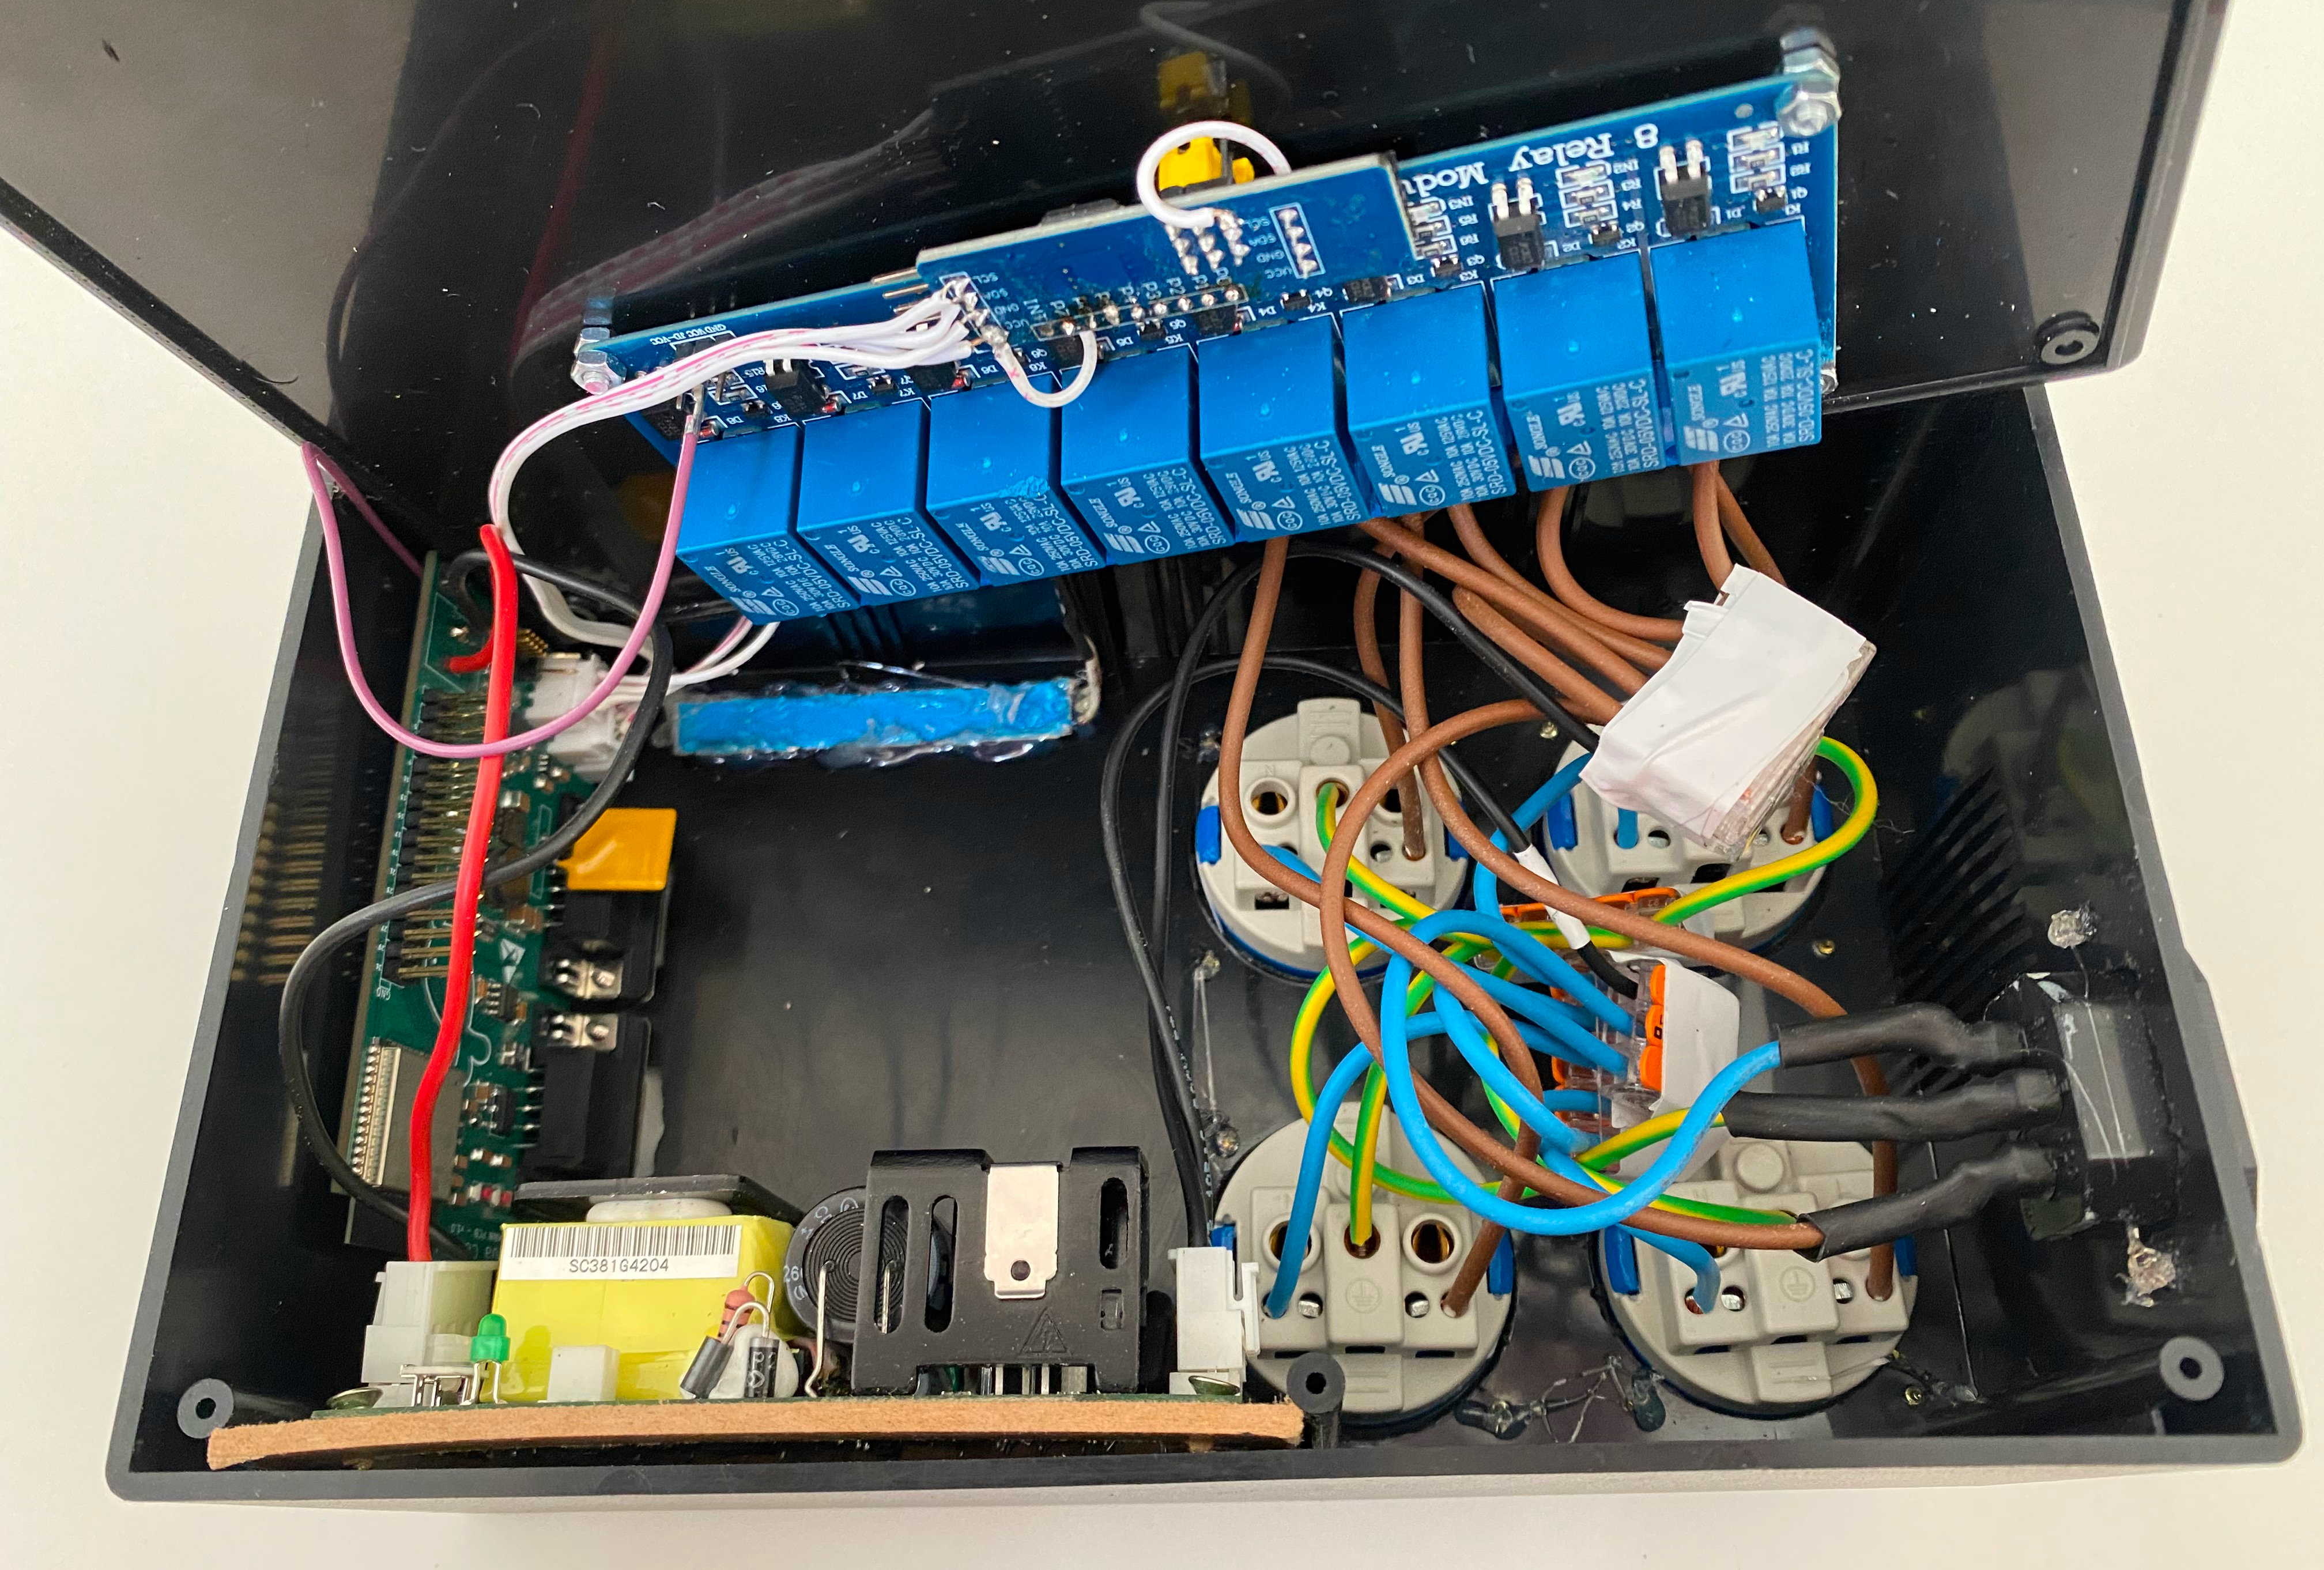
\includegraphics[width=0.8\textwidth]{obrazky/foto/ulozeni.jpeg}
    \caption{Pohled dovnitř šasi řídicí jednotky.}
    \label{fig:obrazky-foto-ulozeni-jpeg}
\end{figure}

\begin{figure}[h!]
    \centering
    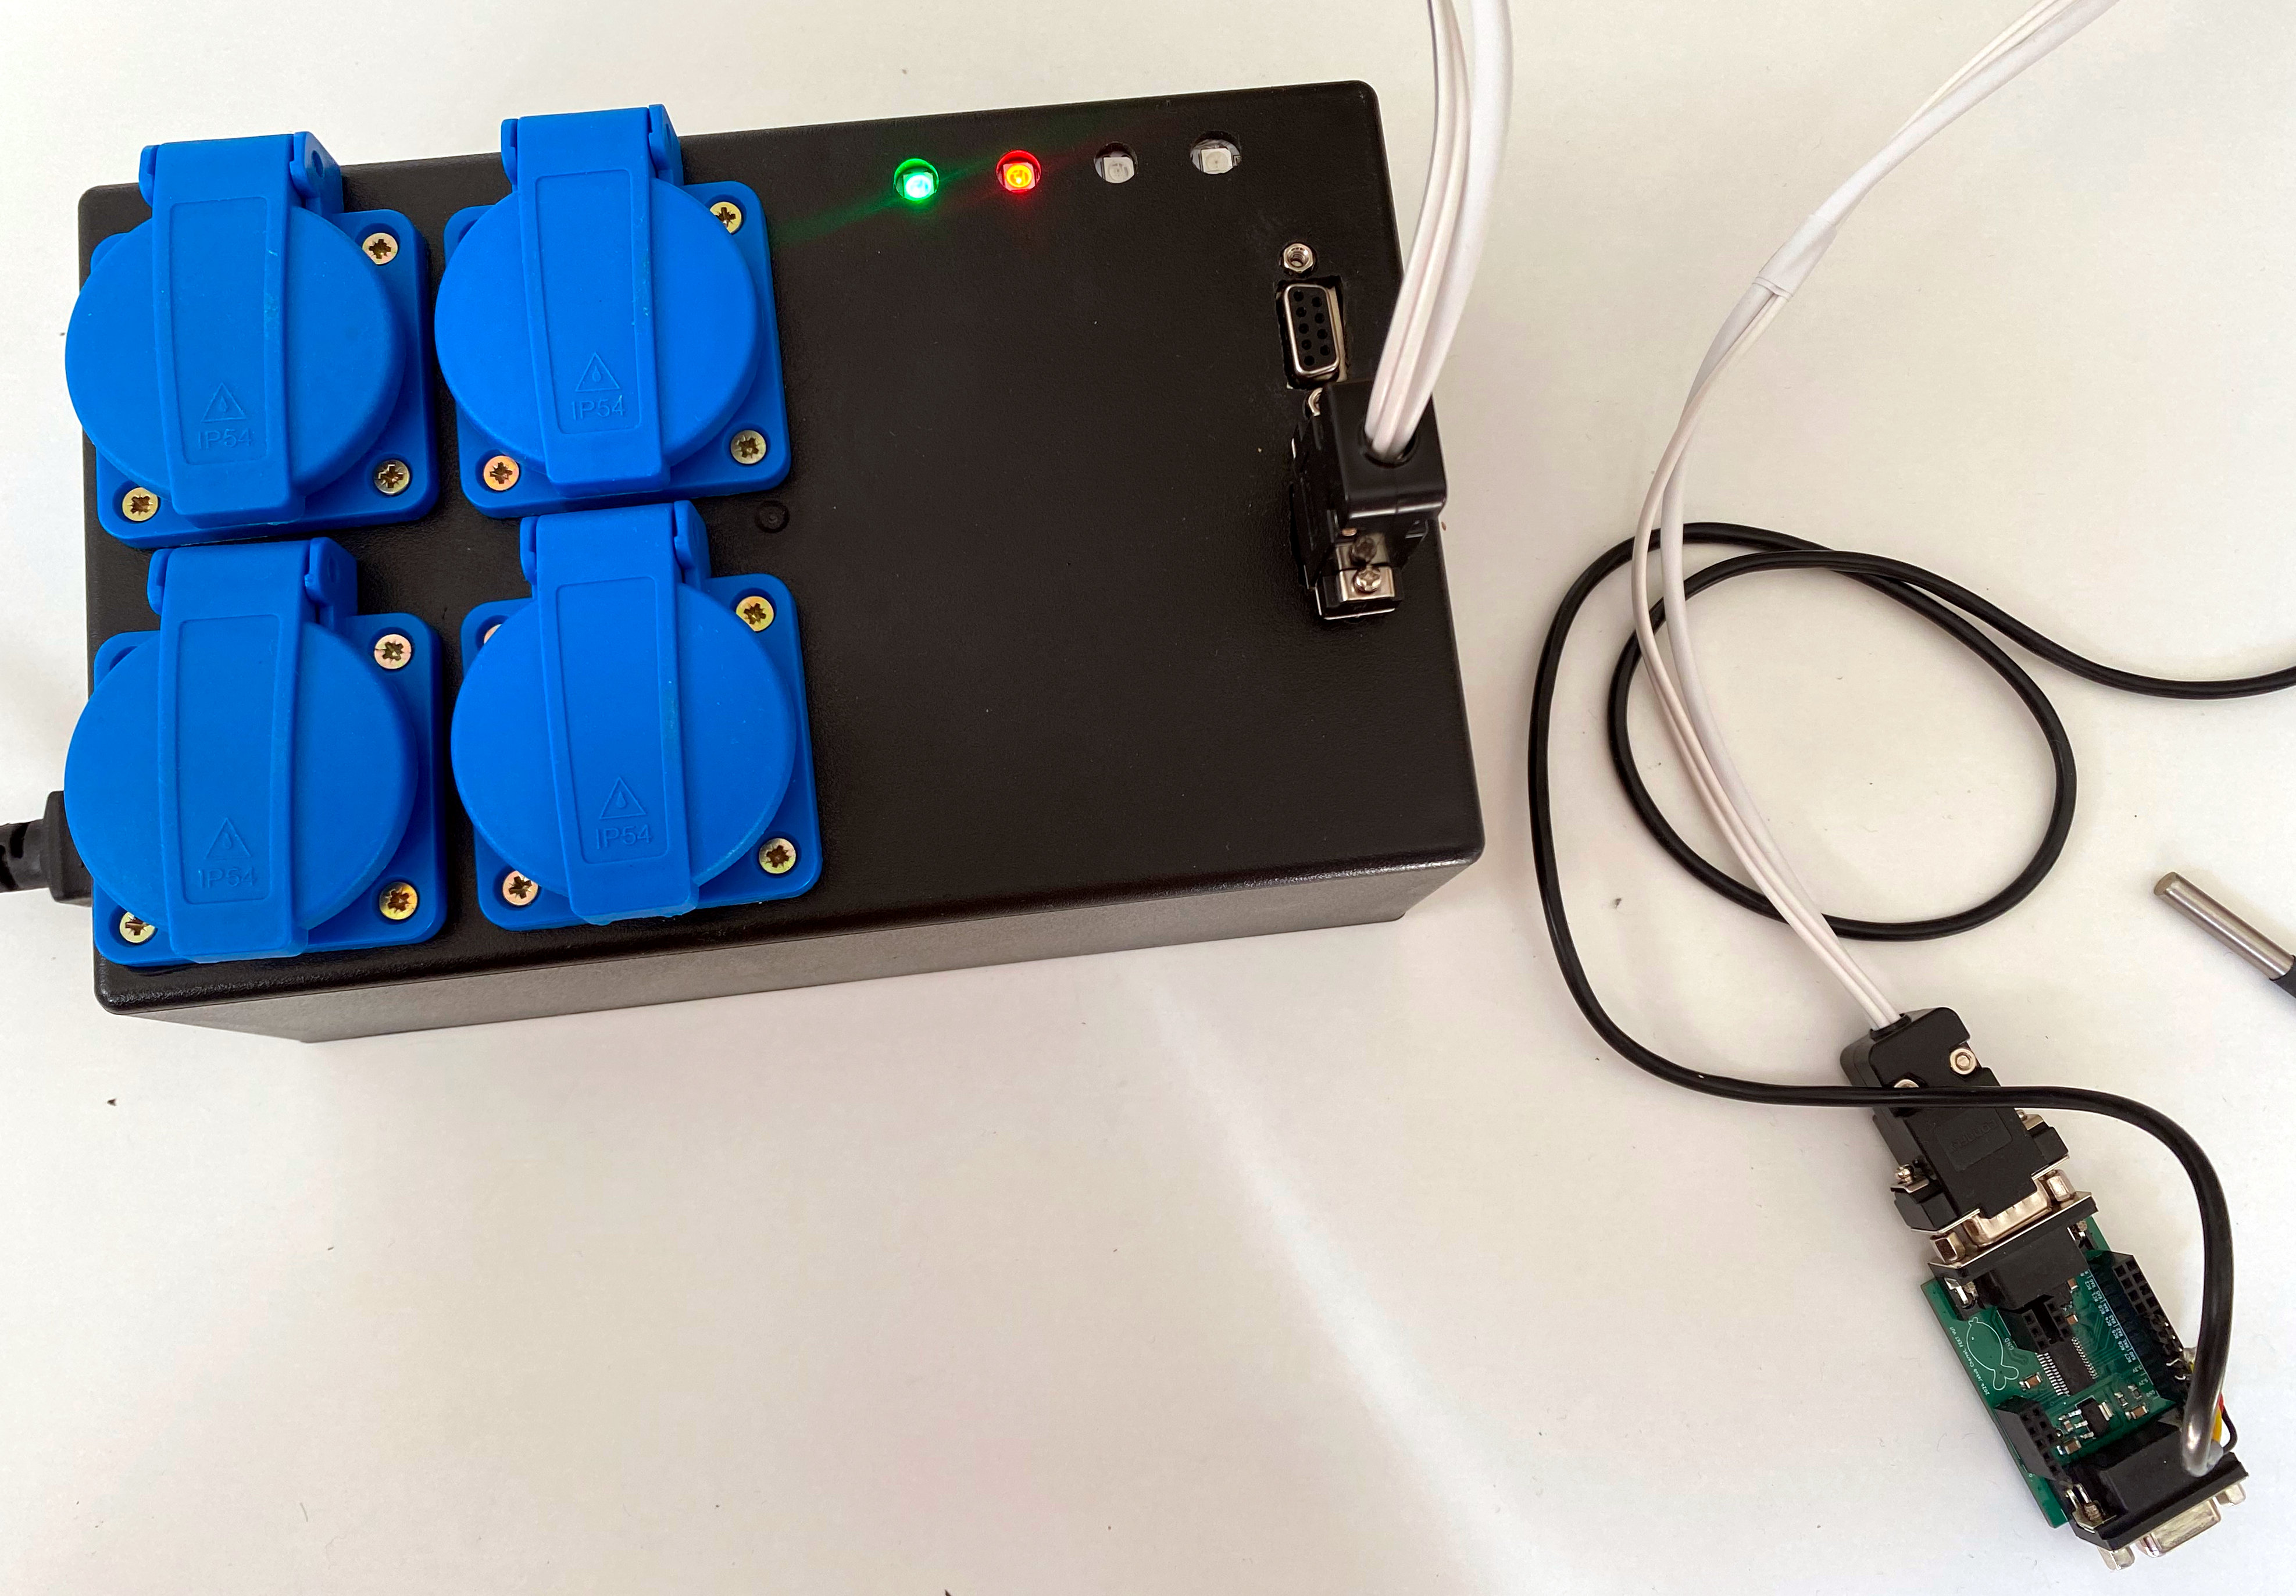
\includegraphics[width=0.8\textwidth]{obrazky/foto/zarizeni_beh.jpeg}
    \caption{Foto šasi řídicí jednotky v běhu.}
    \label{fig:obrazky-foto-zarizeni_beh-jpeg}
\end{figure}


\chapter*{Závěr}
\phantomsection
\addcontentsline{toc}{chapter}{Závěr}

V~rámci bakalářské práce bylo navrženo a sestaveno zařízení, určené k~ovládání běžného domácího akvária. Jedná se o~modulární systém sestávající z~řídicí jednotky a několika propojených modulů, které vzájemně komunikují po sběrnici CAN. K~systému byla také vytvořena jednoduchá webová stránka, přes kterou je možné systém vzdáleně konfigurovat a monitorovat. 

Teoretická část práce se věnuje problematice provozu akvária. Jsou zde rozebrány důležité veličiny, které je potřeba monitorovat a ovládat pro spolehlivé přežití akvarijního ekosystému. Dále se text věnuje průzkumu trhu a používané akvarijní technice. Postupováno je od nezbytného minima pro založení malého akvária, až po systémy zajišťující komplexní automatizaci velkých instalací, složených z~více nádrží.

Na základě provedené rešerše jsou stanoveny požadavky na podobu a funkci vlastního zařízení. Jeho cílem není konkurovat svými možnostmi drahým pokročilým systémům, ale spíše dosáhnout jistého kompromisu mezi cenou a stále dostatečně širokou funkcionalitou k~automatizaci menšího domácího akvária. Samotný návrh systému začíná popisem zvolené architektury, poté jsou podrobněji popsány jednotlivé dílčí části. Byly navrženy tři desky plošných spojů. Řídící jednotka obsahuje spínaný zdroj použitý k~napájení celého systému a mikrokontrolér ESP32 zajišťující kromě samotného řízení také komunikaci skrze síť WiFi. Moduly periferií jsou navrženy jako univerzální platforma, ke které lze připojit různé obvody sensorů nebo akčních členů. Pro plynulé ovládání LED osvětlení byla navržena vlastní deska, kterou lze do této platformy vložit. Ostatní periferie již nebyly tak komplexní a pro připojení sensorů k~univerzální platformě postačila prototypová deska. 

Zvolený způsob komunikace periferií a ovládání přes internet učinil systém velmi komplexní a proto při tvorbě softwaru vznikla řada překážek, kterým bylo potřeba čelit. Klíčové softwarové bloky byly zvládnuty úspěšně. Jednotlivé části systému mezi sebou vzájemně komunikují a možná je i konfigurace systému přes webové rozhraní, ta je navíc zachována v~paměti flash i po restartu zařízení. Stejně tak je zařízení schopné odesílat naměřená data, která si uživatel může na webu zobrazit. Samotný algoritmus řízení akvária ale zatím není dostačující k~úplnému a spolehlivému provozu a řadu funkcí bude potřeba dokončit. 

Jednotlivé dílčí části zařízení byly testovány postupně, z~důvodu nalezených chyb bude dlouhodobý test v~provozu akvária teprve následovat. 

Volba modulární architektury sice návrh zařízení značně zkomplikovala a díky tomuto rozhodnutí nebylo dosaženo všech vytyčených cílů, na druhou stranu je ale zařízení velmi flexibilní a do budoucna má potenciál sloužit nejen jako systém řízení akvária. S~drobným rozšířením může snadno obsloužit vícero oblastní domácí automatizace a stát se tak součástí moderního fenoménu tzv. Smart Home.

% Pro sazbu seznamu literatury použijte jednu z následujících možností

%%%%%%%%%%%%%%%%%%%%%%%%%%%%%%%%%%%%%%%%%%%%%%%%%%%%%%%%%%%%%%%%%%%%%%%%%
%1) Seznam citací definovaný přímo pomocí prostředí literatura / thebibliography

% \begin{thebibliography}{99}
	
% \bibitem{sr72/2017}
% 	VYSOKÉ UČENÍ TECHNICKÉ V~BRNĚ.
% 	\emph{Směrnice č.\,72/2017, Úprava, odevzdávání a~zveřejňování závěrečných prací.}
% 	Online. Brno: VUT v~Brně, 2017.
% 	Úplné znění ke dni 11.\,4.\,2022.
% 	Dostupné z:\\
% 	{\small
% 	\url{https://www.vut.cz/uredni-deska/vnitrni-predpisy-a-dokumenty/smernice-c-72-2017-uprava-odevzdavani-a-zverejnovani-zaverecnych-praci-d161410}.}
% 	[cit.\ 2023-09-27].

% \bibitem{CSN_ISO_690-2022}
%     ÚŘAD PRO TECHNICKOU NORMALIZACI, METROLOGII A~STÁTNÍ ZKUŠEBNICTVÍ.
%     ČSN ISO 690:2022 (01 0197), \emph{Informace a dokumentace -- Pravidla pro bibliografické odkazy a~citace informačních zdrojů.}
%     Čtvrté vydání. Praha, 2022.

% \bibitem{CSN_ISO_7144-1997}
%     ÚŘAD PRO TECHNICKOU NORMALIZACI, METROLOGII A~STÁTNÍ ZKUŠEBNICTVÍ.
%     ČSN ISO 7144 (010161), \emph{Dokumentace -- Formální úprava disertací a~podobných dokumentů.}
% %    24 stran.
%     Praha, 1997.

% \bibitem{CSN_ISO_31-11}
%     ÚŘAD PRO TECHNICKOU NORMALIZACI, METROLOGII A~STÁTNÍ ZKUŠEBNICTVÍ.
%     ČSN ISO 31-11, \emph{Veličiny a~jednotky -- část 11: Matematické znaky a~značky používané ve fyzikálních vědách a~v~technice.}
%     Praha, 1999.

% \bibitem{Farkasova23:CSNISO6902022komentar}
% 	FARKAŠOVÁ, B. et al.
% 	\emph{Výklad normy ČSN ISO 690:2022 (01 0197) účinné od 1.\,12.\,2022}.
% 	 Online. První vydání. 2023.
% 	Dostupné~z:
% 	\url{https://www.citace.com/Vyklad-CSN-ISO-690-2022.pdf}.
% 	[cit.\,2023-09-27].

% \bibitem{pravidla}
%     \emph{Pravidla českého pravopisu}.
% 	1.\ vydání. Olomouc: FIN, 1998.\\
% 	\mbox{ISBN 80-86002-40-3}.

% \bibitem{Walter1999}
% 	WALTER, G.\,G. a SHEN, X.
% 	\emph{Wavelets and Other Orthogonal Systems}.
% 	2.\,vydání, Boca Raton: Chapman\,\&\,Hall/CRC, 2000.
% 	ISBN 1-58488-227-1

% \bibitem{Svacina1999IEEE}
% 	SVAČINA, J.
% 	Dispersion Characteristics of Multilayered Slotlines -- a Simple Approach.
% 	\emph{IEEE Transactions on Microwave Theory and Techniques}.
% 	1999, vol.\,47, no.\,9, s.\,1826--1829. ISSN 0018-9480.

% \bibitem{RajmicSysel2002}
%     RAJMIC, P. a SYSEL, P.
%     Wavelet Spectrum Thresholding Rules.
%     In: \emph{Proceedings of the International Conference Research in Telecommunication Technology}.
%     Žilina: Žilina University, 2002. s.\,60--63. ISBN 80-7100-991-1.

% \end{thebibliography}


%%%%%%%%%%%%%%%%%%%%%%%%%%%%%%%%%%%%%%%%%%%%%%%%%%%%%%%%%%%%%%%%%%%%%%%%%
%%2) Seznam citací pomocí BibTeXu
% Při použití je nutné v TeXnicCenter ve výstupním profilu aktivovat spouštění BibTeXu po překladu.
% Definice stylu seznamu
% \bibliographystyle{unsrturl}
% Pro českou sazbu lze použít styl czechiso.bst ze stránek
% http://www.fit.vutbr.cz/~martinek/latex/czechiso.tar.gz
% \bibliographystyle{czechiso}
% % Vložení souboru se seznamem citací
% \bibliography{text/literatura}

% Následující příkaz je pouze pro ukázku sazby literatury při použití BibTeXu.
% Způsobí citaci všech zdrojů v souboru literatura.bib, i když nejsou citovány v textu.
\nocite{*}


% % Radek approves
\chapter*{Literatura}
\printbibliography[heading=none]

\cleardoublepage
\chapter*{\listofabbrevname}
\phantomsection
\addcontentsline{toc}{chapter}{\listofabbrevname}

\begin{acronym}[iotasdasdsd]

	\acro{iot}[IoT]{Internet of Things -- internet věcí}

	\acro{led}[LED]{Light-Emitting Diode -- dioda emitující světlo}
	\acro{ph}[pH]{Potential of Hydrogen -- potenciál vodíku}
	\acro{co2}[CO\textsubscript{2}]{Carbon Dioxide -- oxid uhličitý}
	\acro{pc}[PC]{Personal Computer -- osobní počítač}
	\acro{wifi}[Wi-Fi]{Wireless Fidelity -- známá bezdrátová síť}
	\acro{spi}[SPI]{Serial Peripheral Interface -- typ sběrnice}
	\acro{i2c}[I\textsuperscript{2}C]{Inter-Integrated Circuit -- typ sběrnice}
	\acro{dps}[DPS]{deska plošných spojů}
	\acro{can}[CAN]{Controller Area Network -- typ sběrnice}
	\acro{cs}[CS]{Chip Select -- signál patřící k~SPI sběrnici}
	\acro{uart}[UART]{Universal Asynchronous Receiver-Transmitter -- typ sběrnice}
	\acro{mcu}[MCU]{Microcontroller Unit -- mikrokontrolér}
	\acro{dc}[DC]{Direct Current -- stejnosměrný proud}
	\acro{mosfet}[MOSFET]{Metal-Oxide-Semiconductor Field-Effect -- typ unipolárního tranzistoru}
	\acro{esd}[ESD]{Electrostatic Discharge -- elektrostatický výboj}
	\acro{vcc}[VCC]{Voltage at the Common Collector -- symbol pro kladné napětí}
	\acro{pptc}[PPTC]{Polymeric Positive Temperature Coefficient -- také značí typ vratné pojistky}
	\acro{gpio}[GPIO]{General Purpose Input/Output -- označení vstupně výstupních pinů MCU}
	\acro{sda}[SDA]{Serial Data Line -- datový signál pro \acs{i2c}}
	\acro{scl}[SCL]{Serial Clock Line -- hodinový signál pro \acs{i2c}}
	\acro{oled}[OLED]{Organic Light-Emitting Diode -- často používaný typ displeje}
	\acro{pwm}[PWM]{Pulse-Width Modulation -- pulzně šířková modulace}
	\acro{adc}[ADC]{Analog to Digital Convertor -- Analogově-digitální převodník}
	\acro{dac}[DAC]{Digital to Analog Convertor -- Digitálně-analogový převodník}
	\acro{vcc}[VCC]{Voltage Common Collector -- napájecí napětí}
	\acro{gnd}[GND]{Ground -- zem, zemnicí vodič}
	\acro{esr}[ESR]{Equivalent Series Resistance -- ekvivalentní sériový odpor}
	\acro{ntc}[NTC]{Negative Temperature Coefficient -- záporný teplotní koeficient}
	\acro{ptc}[PTC]{Positive Temperature Coefficient -- kladný teplotní koeficient}
	\acro{esp-idf}[ESP-IDF]{Espressif IoT Development Framework -- vývojový framework firmy Espressif}
	\acro{hal}[HAL]{Hardware Abstraction Layer -- abstrakční vrstva ve zdrojovém kódu}
	\acro{api}[API]{Application Programming Interface -- aplikační rozhraní}
	\acro{rtos}[RTOS]{Real-Time Operating System -- operační systém reálného času}
	\acro{php}[PHP]{PHP Hypertext Preprocessor -- programovací jazyk}
	\acro{isr}[ISR]{Interrupt Service Routine -- obsluha přerušení}
	\acro{db}[DB]{Database -- databáze}
	\acro{json}[JSON]{JavaScript Object Notation -- formát ukládání a přenosu strukturovaných dat}

\end{acronym}



%%% Začátek příloh
\appendix

%%% Vysázení seznamu příloh
% (vynechejte, pokud máte dvě nebo méně příloh)
\listofappendices

%%% Vložení souboru 'text/prilohy' s přílohami
% Obvykle je přítomen alespoň popis co najdeme na přiloženém médiu
\chapter{Schéma řídící jednotky}
\label{priloha:schema-ridici-jednotka}
\section{Blokové schéma}
\label{priloha:schema-ridici-jednotka-blokove}
	% trim=left bottom right top
	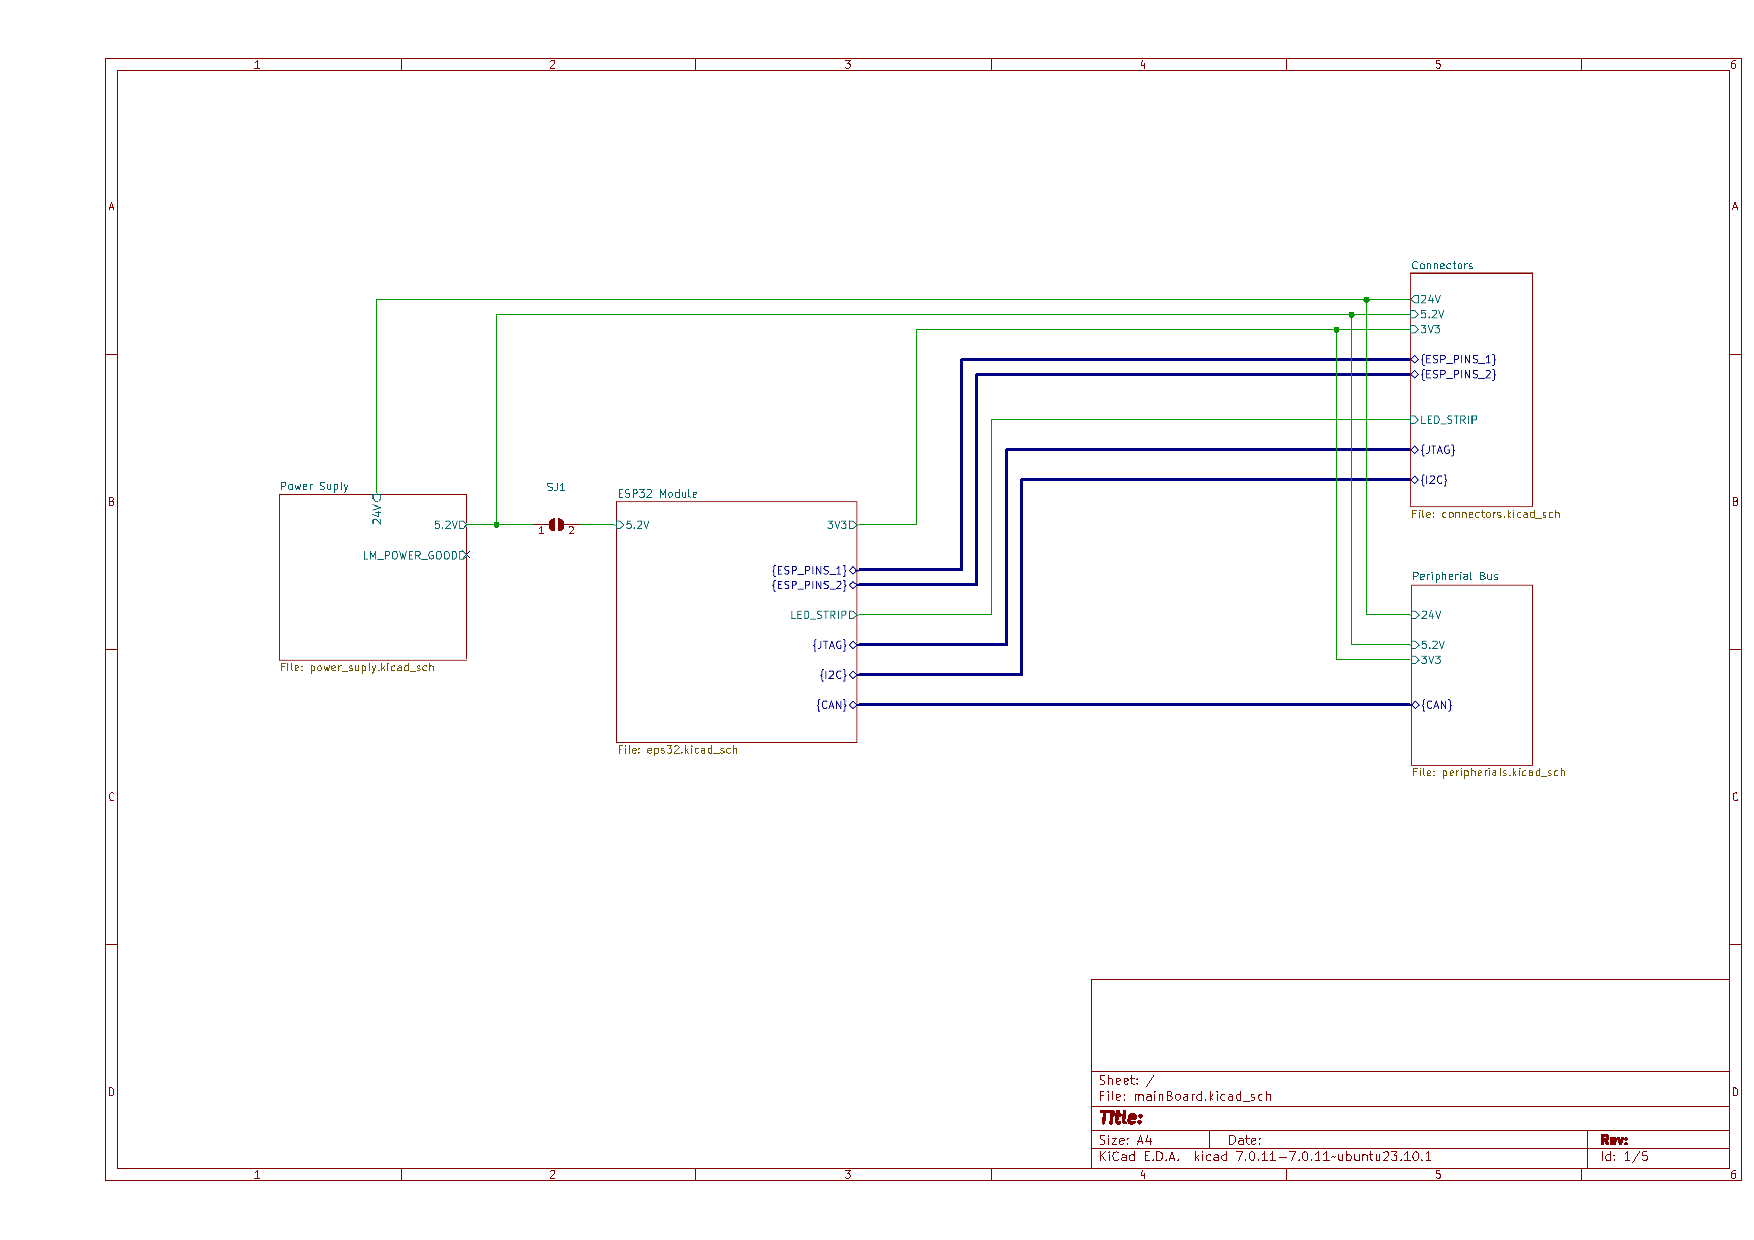
\includegraphics
	[
		width=\textheight, height=0.9\textwidth, keepaspectratio,
		page=1, 
		angle=90,
		trim=1.5cm 1cm 0cm 1cm, 
		clip
	]{obrazky/exportovane/main-board-schematic.pdf}

	\section{Zapojení MCU}
\label{priloha:schema-ridici-jednotka-mcu}
	% trim=left bottom right top
	\includegraphics
	[
		width=\textheight, height=\textwidth, keepaspectratio,
		page=2, 
		angle=90,
		trim=1.5cm 1cm 0cm 1cm, 
		clip
	]{obrazky/exportovane/main-board-schematic.pdf}

	\section{Napájecí obvod}
\label{priloha:schema-ridici-jednotka-napajeci-obvod}
	% trim=left bottom right top
	\includegraphics
	[
		width=\textheight, height=\textwidth, keepaspectratio,
		page=3, 
		angle=90,
		trim=1.5cm 1cm 0cm 1cm, 
		clip
	]{obrazky/exportovane/main-board-schematic.pdf}

	\section{Konektory}
\label{priloha:schema-ridici-jednotka-konektory}
	% trim=left bottom right top
	\includegraphics
	[
		width=\textheight, height=\textwidth, keepaspectratio,
		page=4, 
		angle=90,
		trim=1.5cm 1cm 0cm 1cm, 
		clip
	]{obrazky/exportovane/main-board-schematic.pdf}

	\section{Sběrnice periferií}
	\label{priloha:schema-ridici-jednotka-periferie}
		% trim=left bottom right top
		\includegraphics
		[
			width=\textheight, height=\textwidth, keepaspectratio,
			page=5, 
			angle=90,
			trim=1.5cm 1cm 0cm 1cm, 
			clip
		]{obrazky/exportovane/main-board-schematic.pdf}


\chapter{Schéma modulu periferií}
\label{priloha:schema-modul-periferii}
	% trim=left bottom right top
	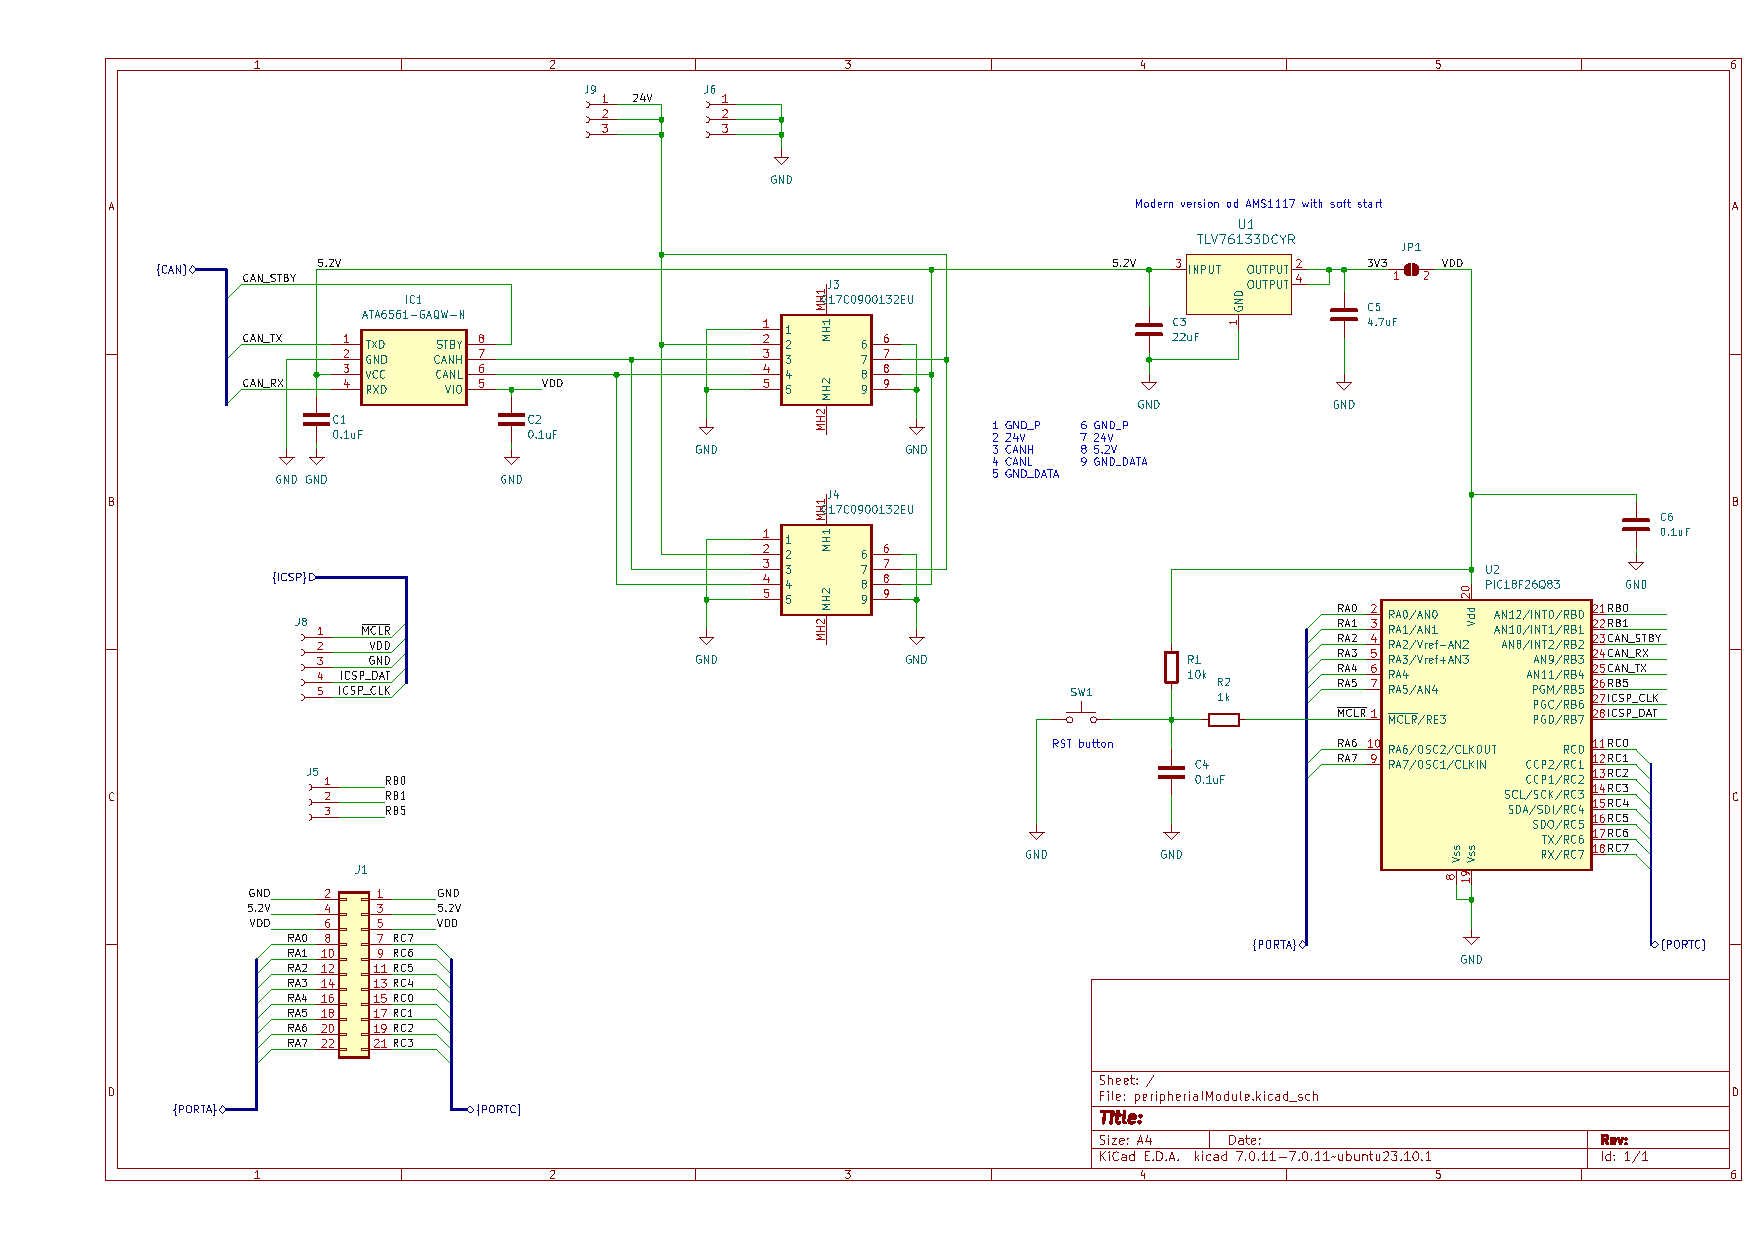
\includegraphics
	[
		width=\textheight, height=\textwidth, keepaspectratio,
		page=1, 
		angle=90,
		trim=1.5cm 1cm 0cm 1cm, 
		clip
	]{obrazky/exportovane/peripherial-module-schematic.pdf}

\chapter{Schéma modulu LED osvětlení}
\label{priloha:schema-led-board}
	% trim=left bottom right top
	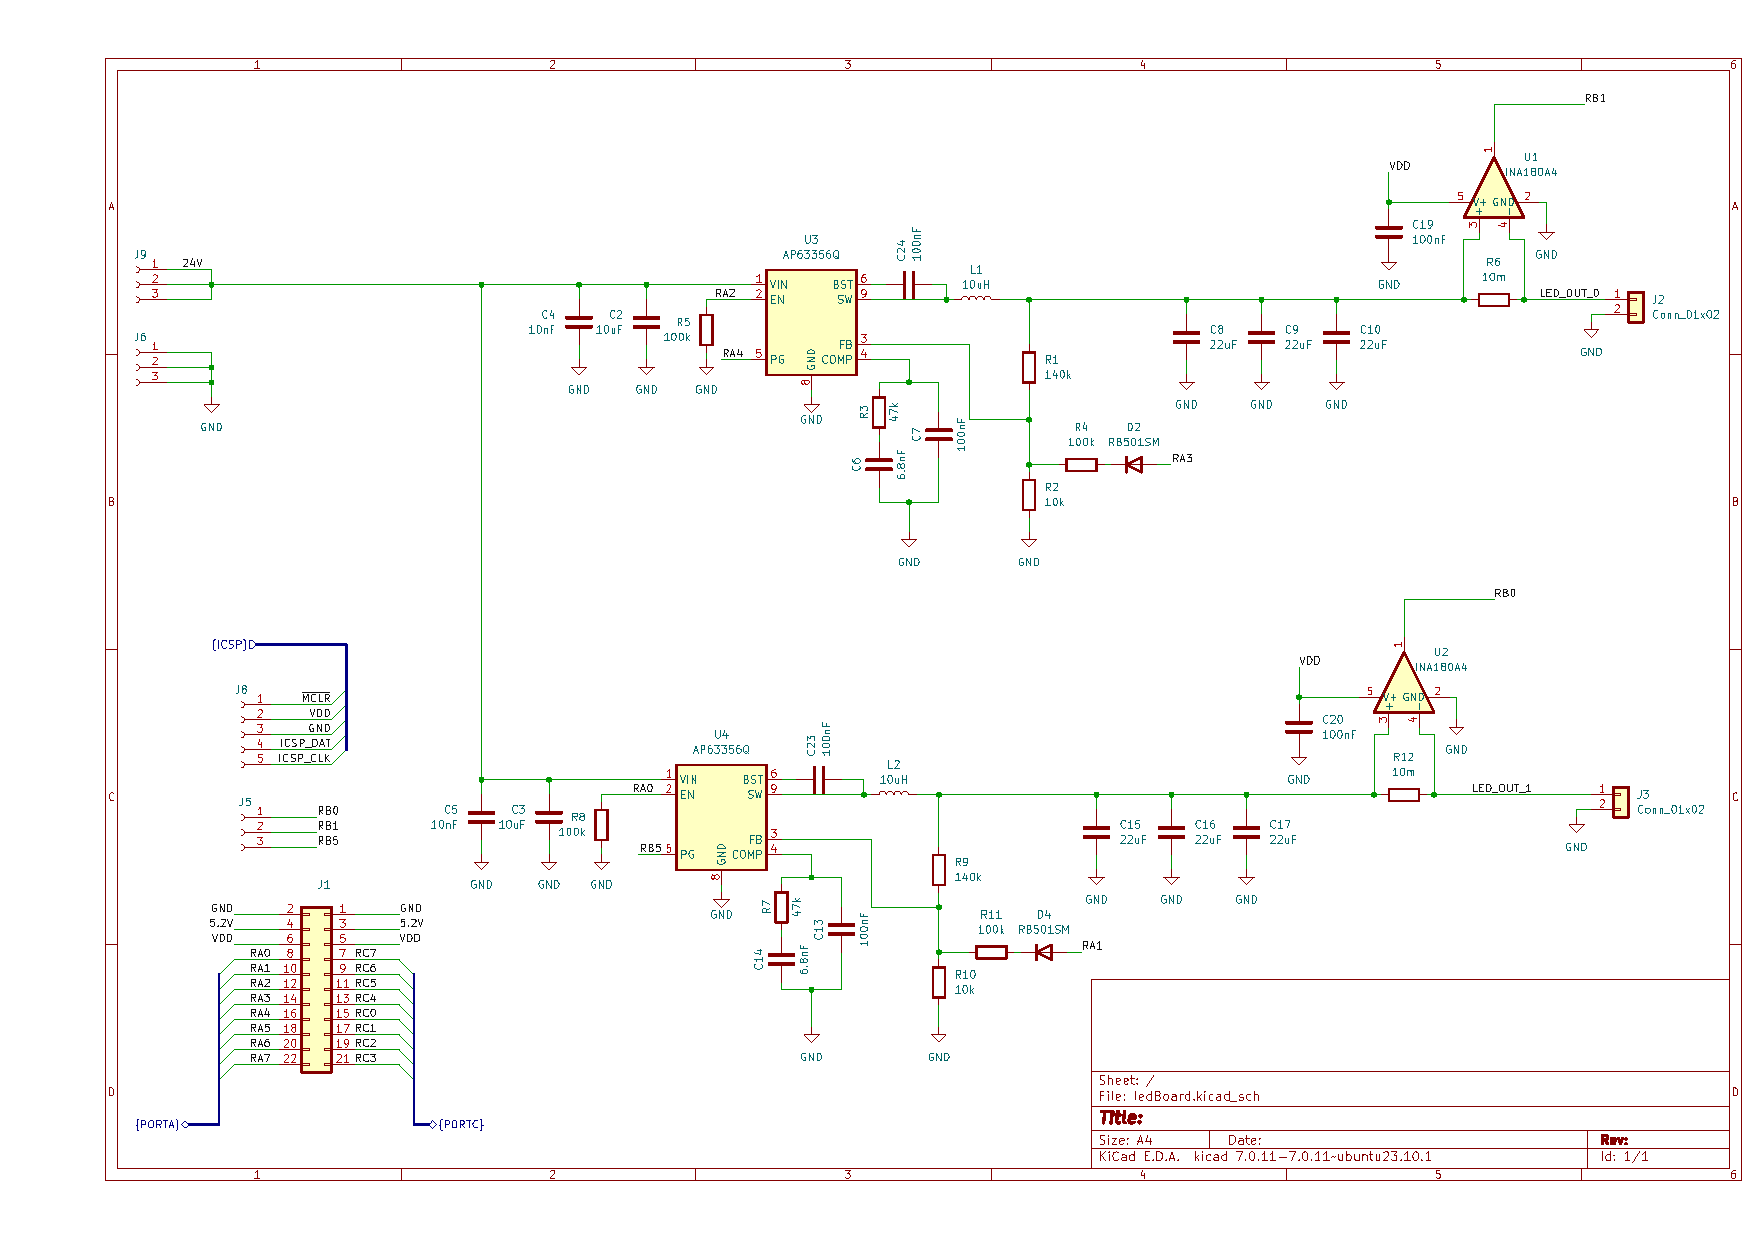
\includegraphics
	[
		width=\textheight, height=\textwidth, keepaspectratio,
		page=1, 
		angle=90,
		trim=1.5cm 1cm 0cm 1cm, 
		clip
	]{obrazky/exportovane/led-board-schematic.pdf}

\end{document}
